\documentclass[a4paper, 12pt, oneside]{article}

%% ─────────────────────────────────────────
%%  ENCODING & FONTS
%% ─────────────────────────────────────────
\usepackage[utf8]{inputenc}
\usepackage[T1]{fontenc}
\usepackage{microtype}

%% ALTEN Brandbook 2025 — main font is Metropolis; in its absence the
%% brand prescribes Arial or Calibri. Carlito is the metric-compatible
%% free Calibri, so the whole document is set in it.
\usepackage[sfdefault,lining]{carlito}

%% ─────────────────────────────────────────
%%  ALTEN BRAND COLOURS (Brandbook EN, Sept. 2025)
%% ─────────────────────────────────────────
\usepackage{xcolor}
% Main trio
\definecolor{altenAzure}{HTML}{008BD2}   % Azure blue
\definecolor{altenNavy}{HTML}{043962}    % Navy blue — running text colour
\definecolor{altenOchre}{HTML}{FFDA65}   % Ochre yellow
% Official shades
\definecolor{altenAzureDark}{HTML}{176F98}
\definecolor{altenAzureLight}{HTML}{7DCAED}
\definecolor{altenAzurePale}{HTML}{B2E0F5}
\definecolor{altenNavyShade}{HTML}{4A617D}
\definecolor{altenOchreDark}{HTML}{FFBA00}
\definecolor{altenOchrePale}{HTML}{FFEF86}
% Greyscale / bluescale (backgrounds, lines, secondary text)
\definecolor{altenGreyBg}{HTML}{EBECF0}
\definecolor{altenGreyLine}{HTML}{CDCEDA}
\definecolor{altenGreyText}{HTML}{8C8C9A}
\definecolor{altenBlueBg}{HTML}{EBF3F9}
\definecolor{altenBlueBg2}{HTML}{DAE8F3}
\definecolor{altenBlueBg3}{HTML}{CBEAF8}

%% Coloured section headings (azure titles on navy text, per charter)
\usepackage{sectsty}
\sectionfont{\color{altenNavy}}
\subsectionfont{\color{altenAzureDark}}
\subsubsectionfont{\color{altenAzureDark}}
\paragraphfont{\color{altenNavy}}

%% ─────────────────────────────────────────
%%  PAGE STYLE
%% ─────────────────────────────────────────
\pagestyle{plain}

\usepackage{fancyhdr}
\fancypagestyle{plain}{
    \fancyhf{}
    \fancyfoot[R]{\ShortTitle\\\textbf{Company Confidential}}
    \fancyfoot[L]{ALTEN\\Innovation Department}
    \renewcommand{\headrulewidth}{0pt}
    \renewcommand{\footrulewidth}{1pt}
}

%% ─────────────────────────────────────────
%%  PARAGRAPH LAYOUT — uniform spacing, no indents
%%  (fixes irregular tabulation at paragraph starts)
%% ─────────────────────────────────────────
\usepackage[skip=8pt plus 2pt, indent=0pt]{parskip}

%% ─────────────────────────────────────────
%%  TOC DEPTH
%% ─────────────────────────────────────────
\setcounter{tocdepth}{3}
\setcounter{secnumdepth}{3}

%% ─────────────────────────────────────────
%%  BIBLIOGRAPHY — biblatex ISO-690
%% ─────────────────────────────────────────
\usepackage[
    style       = iso-authoryear,
    backend     = biber,
    sorting     = nyt,
    maxbibnames = 3,
    minbibnames = 1,
    giveninits  = true,
    urldate     = iso,
]{biblatex}
\addbibresource{Utilities/Bibliography.bib}
\usepackage[nottoc,numbib]{tocbibind}

%% ─────────────────────────────────────────
%%  GLOSSARY
%% ─────────────────────────────────────────
\usepackage[acronym, section=subsection]{glossaries}
\makenoidxglossaries{}
%% ─────────────────────────────────────────────────────────────────────────
%%  ACRONYMS
%% ─────────────────────────────────────────────────────────────────────────
\newacronym{ahp}{AHP}{Analytic Hierarchy Process}
\newacronym{bst}{BST}{Bilan Scientifique et Technique}
\newacronym{bwm}{BWM}{Best-Worst Method}
\newacronym{ci}{CI}{Consistency Index}
\newacronym{cr}{CR}{Consistency Ratio}
\newacronym{csrd}{CSRD}{Corporate Sustainability Reporting Directive}
\newacronym{dag}{DAG}{Directed Acyclic Graph}
\newacronym{din}{DIN}{Direction Innovation Num\'erique}
\newacronym{disco}{DISCO}{Supply Chain Illustrator (Digital Twin, DIN ALTEN)}
\newacronym{dt}{DT}{Digital Twin}
\newacronym{fbwm}{F-BWM}{Fuzzy Best-Worst Method}
\newacronym{glec}{GLEC}{Global Logistics Emissions Council}
\newacronym{hgv}{HGV}{Heavy Goods Vehicle}
\newacronym{iot}{IoT}{Internet of Things}
\newacronym{ipg}{IPG}{Itinerary Performance Index}
\newacronym{kpi}{KPI}{Key Performance Indicator}
\newacronym{lppl}{LPPL}{Log-Periodic Power Law}
\newacronym{mcdm}{MCDM}{Multi-Criteria Decision-Making}
\newacronym{mts}{MTS}{Manchester Triage System}
\newacronym{pi}{PI}{Physical Internet}
\newacronym{promethee}{PROMETHEE}{Preference Ranking Organisation METHod for Enrichment Evaluation}
\newacronym{ri}{RI}{Random Index (Saaty)}
\newacronym{sc}{SC}{Supply Chain}
\newacronym{tmt}{TMT}{Temporal Motivational Theory}
\newacronym{tfn}{TFN}{Triangular Fuzzy Number}
\newacronym{tts}{TTS}{Time To Service}
\newacronym{ttr}{TTR}{Time To Recovery}
\newacronym{vecto}{VECTO}{Vehicle Energy Consumption calculation TOol}
\newacronym{xai}{XAI}{Explainable Artificial Intelligence}

%% ─────────────────────────────────────────────────────────────────────────
%%  MAIN GLOSSARY ENTRIES (key mathematical symbols and concepts)
%% ─────────────────────────────────────────────────────────────────────────
\newglossaryentry{ur}{
    name={$U_r(t)$},
    description={Real (operationally computable) urgency at time $t$: a
        weighted probabilistic OR aggregation of six local KPI blocks
        (time, capacity, performance, risk, cost, CO2), $U_{r,\text{local}}
        = 1-\prod_m(1-u_m)^{\omega_m}$, propagated upstream across the
        supply chain DAG through the leaky coefficients $\beta_{ji}$}}

\newglossaryentry{ud}{
    name={$U_d$},
    description={Declared urgency, a scalar $\in [0,1]$ elicited from the
        human operator via an AHP or Fuzzy-BWM questionnaire, propagated
        downstream across the supply chain DAG through the leaky
        coefficients $\gamma_{ik}$}}

\newglossaryentry{at}{
    name={$A(t)$},
    description={Adequacy score at time $t$, quantifying the asymmetric
        Prospect Theory penalty between $U_d$ and $U_r(t)$:
        $A = 100\times(\exp(-\text{penalty})-\text{floor})/(1-\text{floor})$
        with $\text{penalty}=\lambda_{\text{under}}H^{\alpha}+
        \lambda_{\text{over}}F^{\alpha}$, $\in [0,100]$}}

\newglossaryentry{deltau}{
    name={$\Delta U(t)$},
    description={Raw urgency mismatch: $U_d - U_r(t) \in (-1,1)$; positive
        = over-triage (false urgency), negative = under-triage
        (hidden risk)}}

\newglossaryentry{fh}{
    name={$F$, $H$},
    description={False urgency $F=[U_d-U_r]_+$ (unjustified panic) and
        hidden risk $H=[U_r-U_d]_+$ (silent danger), the two asymmetrically
        penalised pathologies underlying $A(t)$}}

\newglossaryentry{omegam}{
    name={$\omega_m$},
    description={Aggregation weight of KPI block $m$ in the real urgency
        noisy-OR aggregation, reused unchanged as the PROMETHEE~II
        criteria weight for network-wide node outranking}}

\newglossaryentry{deltaurcrit}{
    name={$\Delta U_{r,\text{final}}$},
    description={Network criticality delta: the increase in real urgency
        propagated to final-customer nodes when a given node's local
        urgency is forced to saturation in a systematic shock simulation}}


%% ─────────────────────────────────────────
%%  MATHEMATICS
%% ─────────────────────────────────────────
\usepackage{amsmath, amssymb, mathtools}

%% ─────────────────────────────────────────
%%  MEDIA / GRAPHICS
%% ─────────────────────────────────────────
\usepackage{rotating}
\usepackage{graphicx}
\usepackage{caption}
\usepackage[hidelinks]{hyperref}
\usepackage{svg}

%% ─────────────────────────────────────────
%%  TABLES
%% ─────────────────────────────────────────
\usepackage{tabularx, array, booktabs, multirow, longtable, float}
\renewcommand{\tabularxcolumn}[1]{m{#1}}

%% ─────────────────────────────────────────
%%  LISTS
%% ─────────────────────────────────────────
\usepackage{enumitem}
\setitemize{parsep=0pt, partopsep=0pt}
\setenumerate{parsep=0pt, partopsep=0pt}

%% ─────────────────────────────────────────
%%  CODE LISTINGS
%% ─────────────────────────────────────────
\usepackage{listings}

%% ─────────────────────────────────────────
%%  HYPERLINKS
%% ─────────────────────────────────────────
\hypersetup{
    colorlinks  = true,
    linkcolor   = altenAzure,
    filecolor   = altenAzure,
    urlcolor    = altenAzure,
    citecolor   = altenAzure,
    pdfpagemode = FullScreen,
}

%% ─────────────────────────────────────────
%%  TOC SPACING
%% ─────────────────────────────────────────
\makeatletter
\pretocmd{\chapter}{\addtocontents{toc}{\protect\addvspace{15\p@}}}{}{}
\pretocmd{\section}{\addtocontents{toc}{\protect\addvspace{5\p@}}}{}{}
\pretocmd{\subsection}{\addtocontents{toc}{\protect\addvspace{5\p@}}}{}{}
\pretocmd{\subsubsection}{\addtocontents{toc}{\protect\addvspace{5\p@}}}{}{}
\makeatother

%% ─────────────────────────────────────────
%%  COLOURED BOXES
%% ─────────────────────────────────────────
\usepackage[strict]{changepage}
\usepackage{framed}

\colorlet{definitionshade}{altenBlueBg2}
\newenvironment{definitionBox}{%
  \def\FrameCommand{%
    \hspace{1pt}%
    {\color{altenNavy}\vrule width 2pt}%
    {\color{definitionshade}\vrule width 4pt}%
    \colorbox{definitionshade}%
  }%
  \MakeFramed{\advance\hsize-\width\FrameRestore}%
  \noindent\hspace{-4.55pt}%
  \begin{adjustwidth}{}{7pt}%
  \vspace{2pt}\vspace{2pt}%
}{\vspace{2pt}\end{adjustwidth}\endMakeFramed}

\colorlet{exampleShade}{altenBlueBg}
\newenvironment{exampleBox}{%
  \def\FrameCommand{%
    \hspace{1pt}%
    {\color{altenAzure}\vrule width 2pt}%
    {\color{exampleShade}\vrule width 4pt}%
    \colorbox{exampleShade}%
  }%
  \MakeFramed{\advance\hsize-\width\FrameRestore}%
  \noindent\hspace{-4.55pt}%
  \begin{adjustwidth}{}{7pt}%
  \vspace{2pt}\vspace{2pt}%
}{\vspace{2pt}\end{adjustwidth}\endMakeFramed}

%% Brand charter excludes red: attention accents use ochre yellow instead
\colorlet{attentionShade}{altenOchrePale!45!white}
\newenvironment{attentionBox}{%
  \def\FrameCommand{%
    \hspace{1pt}%
    {\color{altenOchreDark}\vrule width 2pt}%
    {\color{attentionShade}\vrule width 4pt}%
    \colorbox{attentionShade}%
  }%
  \MakeFramed{\advance\hsize-\width\FrameRestore}%
  \noindent\hspace{-4.55pt}%
  \begin{adjustwidth}{}{7pt}%
  \vspace{2pt}\vspace{2pt}%
}{\vspace{2pt}\end{adjustwidth}\endMakeFramed}

%% ─────────────────────────────────────────
%%  FIGURE PLACEHOLDERS — red boxes describing figures
%%  to be hand-drawn, then swapped for \includegraphics
%% ─────────────────────────────────────────
\newcommand{\figuretodraw}[3]{%
  \begin{figure}[H]
    \centering
    \fcolorbox{red}{red!4}{%
      \parbox{0.9\linewidth}{%
        \centering\color{red}%
        \textbf{[FIGURE TO DRAW]}\\[5pt]
        \small #1\par
      }%
    }
    \caption{#2}
    \label{#3}
  \end{figure}
}

%% ─────────────────────────────────────────
%%  COMMENTS
%% ─────────────────────────────────────────
\usepackage{comment}

%%%%%%%%%%%%%%%%%%%%%%%%%%%%%%%%%%%%%%%%%%%%%%%%%%%%%%%%%%%
%% BEGIN OF DOCUMENT
%%%%%%%%%%%%%%%%%%%%%%%%%%%%%%%%%%%%%%%%%%%%%%%%%%%%%%%%%%%

\begin{document}

%% ALTEN charter: running text is navy blue, never black
\color{altenNavy}

\newcommand{\ShortTitle}{DISCO: Urgency Adequacy BST 2026}

\begin{titlepage}
    \centering

    \vspace*{1cm}

    {\Large\bfseries
        Adequacy Score Between Declared and Real Urgency\\[4pt]
        in a Digital Smart Green Supply Chain\par}

    \vspace{0.35cm}
    {\normalsize R\&D BST, Digital Smart Green Supply Chain: Planning Score\par}

    \vspace{0.7cm}

    \noindent
    \begin{minipage}[c]{.5\textwidth}
        \centering
        
\includegraphics[height=1.8cm, keepaspectratio]{Images/0.Cover/LogoALTEN.png}
    \end{minipage}%
    \begin{minipage}[c]{.5\textwidth}
        \centering
        
\includegraphics[height=1.8cm, keepaspectratio]{Images/0.Cover/LogoDIN.png}
    \end{minipage}

    \vspace{0.7cm}

        \normalsize
        {\raggedright
        \renewcommand{\tabularxcolumn}[1]{p{#1}}
        \setlength{\tabcolsep}{0pt}
        \begin{tabularx}{\textwidth}{@{}>{\raggedright\arraybackslash}p{0.33\textwidth}>{\raggedright\arraybackslash}X@{}}
        \multicolumn{2}{l}{\textbf{Author}} \\[2pt]
        \multicolumn{2}{l}{John Hoarau, R\&D Intern,
            Direction Innovation Num\'erique, ALTEN} \\[7pt]

        \multicolumn{2}{l}{\textbf{Industrial Supervisors}} \\[2pt]
        S\'ebastien Perthuisot
            & Directeur de Programme de Recherche et Expert
              Qualit\'e \& Supply Chain, DIN, Groupe ALTEN, \texttt{s.perthuisot@alten.fr} \\[4pt]
        Fabien Jules
            & Charg\'e Innovation, ALTEN,
              \texttt{stage.innovation.center@alten.fr} \\[7pt]

        \multicolumn{2}{l}{\textbf{Academic Supervisor (ESTIA)}} \\[2pt]
        David Gomez
            & Professeur en Informatique,
              ESTIA Institut de Technologie, Bidart,
              \texttt{d.gomez@estia.fr} \\[7pt]

        \multicolumn{2}{l}{\textbf{Academic Supervisor (Cranfield)}} \\[2pt]
        Peter Sherar
            & Dr, Centre for Computational Engineering Sciences,
              Cranfield University,
              \texttt{p.sherar@cranfield.ac.uk} \\
        \end{tabularx}
        }

    \vfill

    {\Large ALTEN\\Innovation Department\par}

    \vspace{0.8cm}
    {\large 2026\\\textbf{Company Confidential}\par}

\end{titlepage}


\clearpage
\section*{Remerciements}
\label{sec:remerciements}
\addcontentsline{toc}{section}{Remerciements}
Je tiens à remercier l'ensemble des personnes qui ont accompagné le déroulement de cette opération de R\&D au sein de la Direction Innovation Numérique d'ALTEN.

Je remercie tout particulièrement \textbf{Sébastien Perthuisot}, Directeur de Programme de Recherche et Expert Qualité \& Supply Chain à la DIN, pour son encadrement industriel, la confiance accordée sur l'orientation scientifique du sujet, et ses relectures exigeantes qui ont fait progresser la rigueur du modèle. Je remercie également \textbf{Fabien Jules}, Chargé Innovation à ALTEN, pour son suivi régulier et son aide précieuse dans l'intégration de ce travail au programme Smart Green Supply Chain.

Je remercie mes encadrants académiques, \textbf{David Gomez}, Professeur en Informatique à l'ESTIA, et \textbf{Peter Sherar}, du Centre for Computational Engineering Sciences de Cranfield University, pour leurs conseils méthodologiques et le cadrage académique apporté à ce mémoire.

Enfin, je remercie l'ensemble de l'équipe de la Direction Innovation Numérique pour son accueil et les échanges qui ont nourri ce travail tout au long du stage.

%% NOTE (à personnaliser) : ajouter ici toute personne supplémentaire à
%% remercier (collègues, famille, relecteurs) avant la version finale.


\clearpage
\tableofcontents

\clearpage
\listoffigures
\addcontentsline{toc}{section}{List of Figures}

\clearpage
\listoftables
\addcontentsline{toc}{section}{List of Tables}

\clearpage
\section*{Abstract}
\label{sec:abstract}
\addcontentsline{toc}{section}{Abstract}
Modern supply chains operating under the Physical Internet paradigm face a fundamental signal-quality gap: the urgency declared by operators often diverges from the physically computable real urgency. This leads to over-triage (resource waste) and under-triage (hidden rupture risk). In Supply Chain~4.0 contexts marked by volatility and multi-tier dependencies, no existing digital twin architecture fully corrects this cognitive bias while propagating it consistently across a supplier network.

This report summarises a R\&D internship that proposes a cognitive adequacy score $A(t) \in [0, 100]$ to measure and correct the gap between declared operator urgency and a multi-block, DAG-propagated digital twin real urgency $U_r(t)$. The approach combines pairwise elicitation (AHP, Fuzzy Best-Worst Method) for declared urgency, a noisy-OR aggregation of six operational KPI blocks for real urgency, PROMETHEE~II outranking and systematic shock simulation for network-wide criticality, and a calibrated event engine for keeping the underlying KPI state current. The framework is implemented in Python and operated as a persistent, multi-tenant digital twin exercised through a weekly-cadence serious game, with its adequacy signal validated empirically against recorded operational outcomes.


\clearpage
\section*{R\'esum\'e}
\label{sec:resume}
\addcontentsline{toc}{section}{R\'esum\'e}
Les chaînes logistiques modernes opérant dans les réseaux de l'Internet Physique font face à un écart fondamental de qualité de signal~: l'urgence déclarée par les opérateurs diverge souvent de l'urgence réelle physiquement calculable. Il en résulte du sur-triage (gaspillage de ressources) et du sous-triage (risque de rupture caché). Dans des contextes Supply Chain~4.0 marqués par la volatilité et les dépendances multi-rangs, aucune architecture de jumeau numérique existante ne corrige pleinement ce biais cognitif tout en le propageant de manière cohérente sur un réseau de fournisseurs.

Ce mémoire synthétise un stage de R\&D qui propose un score d'adéquation cognitive $A(t) \in [0, 100]$ pour mesurer et corriger l'écart entre l'urgence déclarée par l'opérateur et une urgence réelle $U_r(t)$ multi-blocs, calculée par le jumeau numérique et propagée sur le graphe orienté acyclique du réseau. L'approche combine une élicitation par comparaisons par paires (AHP, Fuzzy Best-Worst Method) pour l'urgence déclarée, une agrégation noisy-OR de six blocs de KPI opérationnels pour l'urgence réelle, le surclassement PROMETHEE~II et une simulation systématique de chocs pour la criticité réseau, ainsi qu'un moteur d'événements calibrés pour maintenir à jour l'état des KPI sous-jacents. Le cadre est implémenté en Python et opéré comme un jumeau numérique persistant et multi-tenant, exercé à travers un serious game à cadence hebdomadaire, avec un service de calibration dédié comparant le signal d'adéquation aux résultats opérationnels enregistrés.


\clearpage
\section{R\&D Operation Context}
\label{sec:Context}
%% ─────────────────────────────────────────────────────────────────────────
\subsection{Internal Research Context}
%% ─────────────────────────────────────────────────────────────────────────

\subsubsection{Smart Green Supply Chain Programme}


The \gls{din} of ALTEN conducts applied R\&D at the
intersection of digital twin technology, logistics optimisation, and sustainable
transport. 

The Smart Green Supply Chain programme~\autocite{benzakour2024history}
articulates three complementary pillars:

\begin{itemize}
    \item \textbf{Lean}: Minimisation of waste (cost, delay, over-stock) through
          pull-flow logic and real-time scheduling.
    \item \textbf{Green}: Minimisation of carbon footprint per transport leg, aligned with the \gls{glec} Framework v3.2~\autocite{smartfreight2023glec} and ISO~14083:2023~\autocite{iso14083}.
    \item \textbf{Predictive}: Anticipation of disruptions through probabilistic modelling and machine learning, consistent with the digital supply chain twin approach~\autocite{ivanov2020digital}.
\end{itemize}

This programme places ALTEN-DIN within the broader Industry~4.0 movement \autocite{kagermann2013industry}, which uses cyber-physical systems, \gls{iot}, and
digital twins to transform reactive supply chains into adaptive, self-organising networks.

The Physical Internet framework~\autocite{montreuil2011toward}, proposing
open, mutualized logistics networks analogous to internet routing protocols, provides the theoretical backdrop for the supply chain simulation environment described below.

\subsubsection{Project: DISCO Digital Twin}

DISCO (Supply Chain Illustrator) is a serious game and digital twin developed by the DIN to simulate a complete supply chain for a fictitious satellite product. It involves
22 component suppliers in domains such as structural assemblies, optical systems, and embedded electronics~\autocite{baxas2025architecture}. Players assume the role of
supply chain buyers and make decisions about supplier selection, transport routes, and factory allocation. The DISCO technology stack is summarised in Table~\ref{tab:disco_stack}.

\begin{figure}[H]
    \centering
    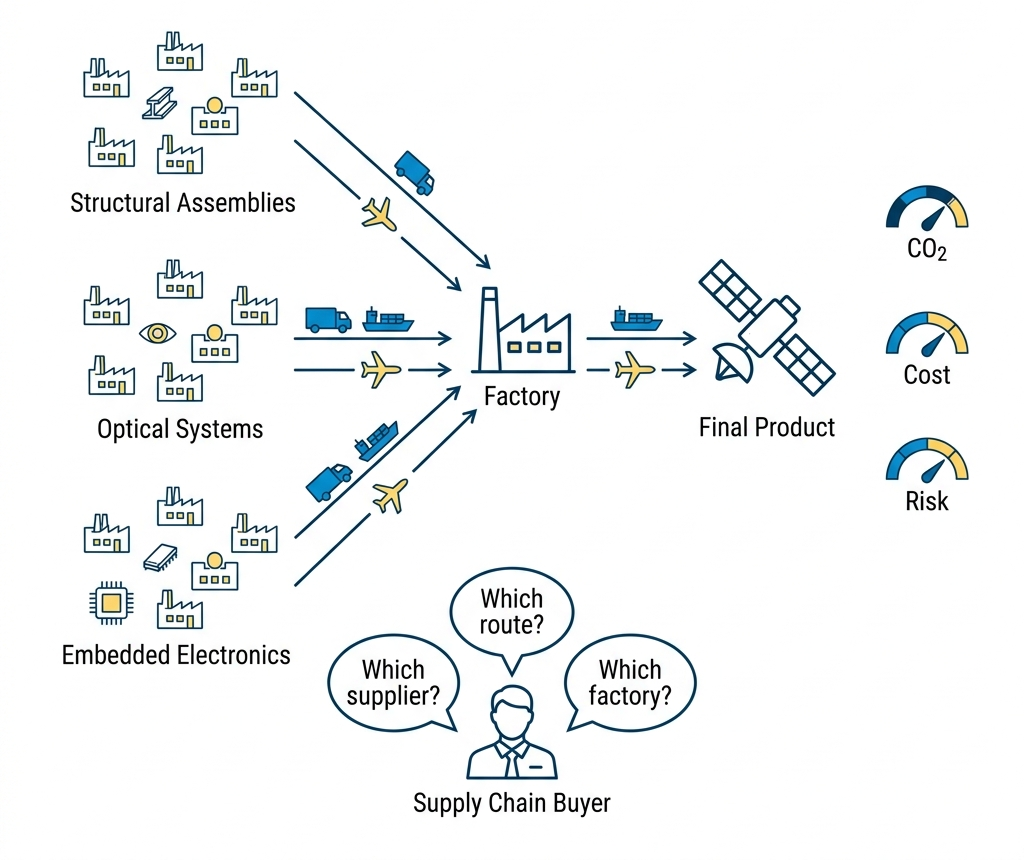
\includegraphics[width=0.85\linewidth]{Images/1.Introduction/disco_map.png}
    \caption{The DISCO serious game: 22 suppliers, transport decisions, and the three scored dimensions.}
    \label{fig:todraw_disco}
\end{figure}

The scoring engine applies Min-Max normalisation over the values of the current game
session:

	\begin{equation}
	    \text{ScoreCO}_2 = 1 + 9 \times \frac{\text{realCO}_2 - \text{co}_{2,\min}}
	                                         {\text{co}_{2,\max} - \text{co}_{2,\min}},
	    \label{eq:score_co2}
	\end{equation}
	
	The operational variables of the CO\textsubscript{2} scoring model are described in Table~\ref{tab:co2_components}.
	
	\begin{table}[H]
	\centering
	\caption{Component definitions for the CO\textsubscript{2} scoring equation.}
	\label{tab:co2_components}
	\small
	\begin{tabularx}{\linewidth}{llX}
	\toprule
	\textbf{Component} & \textbf{Type} & \textbf{Description} \\
	\midrule
	$\text{ScoreCO}_2$ & Dependent variable & Normalized greenhouse gas score on a $[1, 10]$ scale \\
	$\text{realCO}_2$  & Input variable     & Measured carbon emissions on the transport leg \\
	$\text{co}_{2,\min}$ & System parameter  & Minimum historical or target emissions threshold \\
	$\text{co}_{2,\max}$ & System parameter  & Maximum historical or target emissions threshold \\
	\bottomrule
	\end{tabularx}
	\end{table}

with analogous formulae for cost and risk. The scale ranges from 1 to 10, where 1 corresponds to the best possible performance and 10 to the worst.

To support the demonstration and continuous improvement of mature supply chain capabilities, the DISCO digital twin incorporates several specialized modules developed in prior research cycles: The routing module~\autocite{baulain2024internet}, the risk scorer~\autocite{kabouche2025scoring}, the CO\textsubscript{2} quantification methodology~\autocite{cordova2024green}, and the software integration framework~\autocite{auclin2025bst}.


	\begin{table}[ht]
	\centering
	\caption{DISCO technology stack and key parameters.}
	\label{tab:disco_stack}
	\begin{tabularx}{\linewidth}{lX}
	\toprule
	\textbf{Component} & \textbf{Technology / Value} \\
	\midrule
	Backend API    & Spring Boot + Java~21 \\
	Database       & PostgreSQL (Azure) \\
	Frontend       & Angular (localhost:4200) \\
	REST API (test) & \texttt{https://test-disco.altenlabs.net/back/} \\
	Authentication & Player key / Azure AD SSO OAuth2 \\
	Scores computed & CO\textsubscript{2}, Cost, Risk per supplier/itinerary [1–10] \\
	\bottomrule
	\end{tabularx}
	\end{table}

%% ─────────────────────────────────────────────────────────────────────────
\subsubsection{Capitalisation of Prior ALTEN-DIN Research}
%% ─────────────────────────────────────────────────────────────────────────

This R\&D operation is situated within a body of prior DIN research conducted under
the Smart Green Digital Supply Chain programme. These works form the organisational and thematic context of the present
operation; the system delivered here (SupplyScore, Section~\ref{sec:Operations}) is
a standalone Python application and does not integrate with these modules yet.
Their coupling is a stated perspective of the programme, not a
delivered capability.

\textbf{Baxas~\autocite{baxas2025architecture}} defines the DISCO software
architecture, including the \gls{tts}/\gls{ttr} formalisation.

\textbf{Baulain and Dubarry~\autocite{baulain2024internet}} developed the Physical
Internet routing module of DISCO, providing transit times via the HERE Maps API
(Vincenty distances, mandatory 4h30 \gls{hgv} pause compliance) and the Itinerary
Performance Index (\gls{ipg}) normalised in $[0,1]$.

\textbf{Kabouche~\autocite{kabouche2025scoring}} developed the supplier risk scorer
combining delay history, geographic vulnerability, and financial fragility into a
$[1, 10]$ scale.

\textbf{Cordova~\autocite{cordova2024green}} developed the CO\textsubscript{2}
quantification module per route using the GLEC/VECTO methodology with log-normalised
output $\hat{x}_{\text{CO}_2}$.

\textbf{Mondelice~\autocite{mondelice2025tms}} developed the Transport Management
System interface providing real-time transit-time extraction.


%% ─────────────────────────────────────────────────────────────────────────
\subsection{Document Structure}
%% ─────────────────────────────────────────────────────────────────────────

This document is structured as follows. Section~\ref{sec:Problem} formalises the scientific problem, states the operation's objectives, research questions and hypotheses, and outlines the primary research challenges. Section~\ref{sec:SOTA} reviews the state of the art across thematic subsections. Section~\ref{sec:Operations} details the R\&D iterations, the methodology, and the serious-game validation campaign. Finally, Section~\ref{sec:Conclusions} states the documented limitations of the delivered framework and closes with a personal assessment.


\clearpage
\section{Scientific Problem and Obstacles to Overcome}
\label{sec:Problem}
%% ─────────────────────────────────────────────────────────────────────────
\subsection{Relevant Context and Motivating Observations}
%% ─────────────────────────────────────────────────────────────────────────

Modern supply chain operators face simultaneous multi-dimensional assessments (cost, deadline, risk, carbon) where most monitoring and planning tools process one criterion at a time~\autocite{pinedo2012scheduling,chakrabortty2020efficient}, which is precisely why practitioners fall back on judgment-based prioritisation.

This work addresses the layer that comes \emph{before} any planning or scheduling decision, and which the classical literature has not fully investigated: the urgency signal itself is systematically biased at the source and must be measured and corrected before it can safely inform any downstream decision~\autocite{zhu2018mere,rusou2020psychology}.

In a Physical Internet network~\autocite{montreuil2011toward}, where logistics capacity is mutualized across actors, a biased urgency signal propagates and amplifies systemic misallocations. Over-triage (declaring an urgency higher than the physical situation warrants) starves other network tenants, whereas under-triage (declaring an urgency lower than warranted) creates invisible stock rupture risk that cascades downstream~\autocite{li2020exploring,ivanov2020digital}.

While digital twin architectures and real-time decision support systems have demonstrated strong capabilities in operational monitoring, disruption detection, resource reallocation, and order synchronisation~\autocite{ding2023realtime,leung2022digital,hrusovsky2021realtime,karam2022realtime,zhu2025industry5}, they do so primarily by computing the physical operational state of the system. To the best of the present review, existing systems do not appear to explicitly model the gap between a declared client urgency and a computed operational urgency.

The core scientific novelty of this R\&D operation therefore lies in the formal comparison between these declared and computed urgencies, propagated coherently across a multi-tier network. This missing integration motivates the introduction of an urgency adequacy layer in digital operations architectures.

\begin{figure}[H]
    \centering
    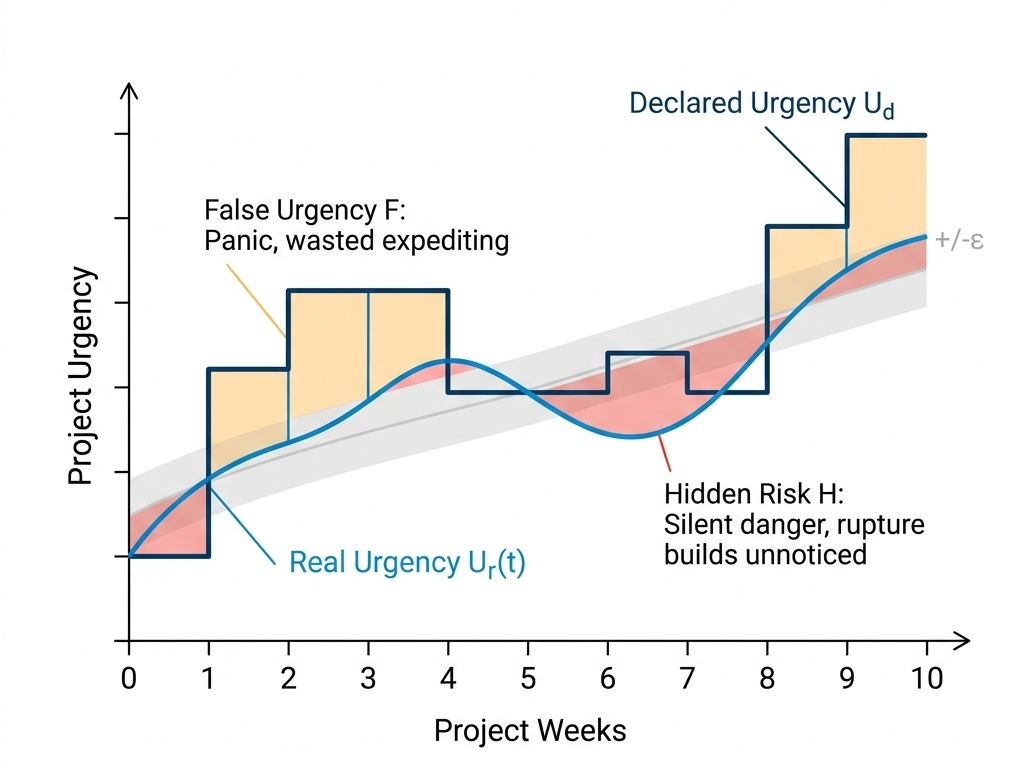
\includegraphics[width=0.85\linewidth]{Images/2.Problem/urgency_gap.png}
    \caption{Conceptual view of the declared vs.\ real urgency gap and its two pathologies. The step line is declared urgency $U_d$ and the smooth curve is real urgency $U_r(t)$; the shaded areas mark where the two mismatch, false urgency $F$ where $U_d$ exceeds $U_r$, hidden risk $H$ where $U_r$ exceeds $U_d$.}
    \label{fig:todraw_gap}
\end{figure}

%% ─────────────────────────────────────────────────────────────────────────
\subsection{Formal Problem Statement}
%% ─────────────────────────────────────────────────────────────────────────

Let $U_d \in [0,1]$ denote the declared urgency and $U_r(t) \in [0,1]$ the real urgency computed from operational data in the digital twin. The core variables and domains are summarized in Table~\ref{tab:problem_vars}.

\begin{table}[H]
\centering
\caption{Core variables and domains.}
\label{tab:problem_vars}
\begin{tabularx}{\linewidth}{lXl}
\toprule
\textbf{Symbol} & \textbf{Meaning} & \textbf{Domain} \\
\midrule
$t$ & Current time (project hours, ISO week granularity) & $\mathbb{R}$ \\
$U_r(t)$ & Physically/operationally computable real urgency & $[0,1]$ \\
$U_d$ & Operator-declared urgency  & $[0,1]$ \\
$\varepsilon$ & Tolerance threshold (cognitive noise band) & $[0,1]$ \\
\bottomrule
\end{tabularx}
\end{table}

The mismatch between both signals is defined as
\begin{equation}
    \Delta U(t) = U_d - U_r(t) \in [-1,\, 1].
    \label{eq:delta_u}
\end{equation}

The components of this mismatch equation are explained in Table~\ref{tab:delta_u_components}.

\begin{table}[H]
\centering
\caption{Component definitions for the urgency discrepancy equation.}
\label{tab:delta_u_components}
\small
\begin{tabularx}{\linewidth}{llX}
\toprule
\textbf{Component} & \textbf{Type} & \textbf{Description} \\
\midrule
$\Delta U(t)$ & Dependent variable & Raw urgency mismatch signal at time $t$ \\
$U_d$         & Input variable     & Urgency level declared subjectively by the human operator \\
$U_r(t)$      & Dynamic variable   & Urgency level computed operationally by the digital twin \\
\bottomrule
\end{tabularx}
\end{table}

A tolerance band $\varepsilon \in [0,1]$ is introduced so that small deviations are not treated as operationally meaningful. In this setting, over-declaration corresponds to $\Delta U(t) > \varepsilon$, under-declaration to $\Delta U(t) < -\varepsilon$, and approximate agreement to $|\Delta U(t)| \le \varepsilon$. Potential consequences of these mismatch conditions are summarized in Table~\ref{tab:pathologies}.

\begin{table}[H]
\centering
\caption{Urgency pathologies and potential consequences.}
\label{tab:pathologies}
\small
\begin{tabularx}{\linewidth}{l >{\raggedright\arraybackslash}X >{\raggedright\arraybackslash}X}
\toprule
\textbf{Condition} & \textbf{Interpretation} & \textbf{Potential consequence} \\
\midrule
$\Delta U(t) > \varepsilon$ & Over-declaration of urgency (false urgency) & Excess expediting, avoidable cost, possible delay for other flows \\[4pt]
$\Delta U(t) < -\varepsilon$ & Under-declaration of urgency (hidden risk) & Hidden lateness or stockout risk, delayed intervention, downstream disruption \\[4pt]
$|\Delta U(t)| \le \varepsilon$ & Acceptable alignment & No material urgency mismatch \\
\bottomrule
\end{tabularx}
\end{table}

An asymmetric treatment of mismatch may be introduced through weights such as $\lambda_{\text{under}} \ge \lambda_{\text{over}}$ when the application context treats under-prioritisation as more harmful than over-prioritisation. This is motivated by operations literature showing that decision errors can generate unequal downstream consequences~\autocite{kim2020admission,diwa2020task}, and by scheduling literature that models differentiated tardiness penalties rather than uniform delay costs~\autocite{baker1982dynamic,chakrabortty2022}. However, the degree of asymmetry is treated here as a design and calibration choice to be validated in the target use case, rather than as a universal property.

%% ─────────────────────────────────────────────────────────────────────────
\subsection{Operation Objectives and Research Questions}
%% ─────────────────────────────────────────────────────────────────────────

The R\&D operation is entitled \textit{``Adequacy Score Between Declared and Real
Urgency in a Smart Green Supply Chain Digital Twin''}. Its three operational objectives are:

\begin{enumerate}[label=\textbf{O\arabic*.}]
    \item Define a multi-block, DAG-propagated real urgency $U_r(t)$ and a cognitive adequacy score $A(t) \in [0, 100]$ to measure the gap between the human planner's declared urgency $U_d$ and the digital twin's operational state.
    \item Develop and implement a network propagation and criticality-driven prioritisation layer, combining PROMETHEE~II outranking with systematic shock simulation, to identify structurally critical nodes.
    \item Validate the adequacy-driven prioritisation logic empirically, through worked scenarios and a calibration service comparing the hidden-risk signal against recorded operational outcomes.
\end{enumerate}

Four research questions structure the scientific approach to these objectives:

\begin{enumerate}[label=\textbf{RQ\arabic*}., leftmargin=*]
  \item \textbf{Multi-block real urgency ($U_r(t)$):}
  How can a physically and operationally grounded real urgency $U_r(t)$ be computed dynamically in a multi-tenant digital twin from heterogeneous KPI blocks (temporal, capacity, performance, risk, cost, environmental), and propagated coherently across a multi-tier supply chain graph?

  \item \textbf{Cognitive adequacy formulation ($A(t)$):}
  How should an adequacy score $A(t)$ be formulated to measure the alignment between operator declared urgency $U_d$ and computed real urgency $U_r(t)$, while asymmetrically penalizing under-triage vs.\ over-triage, and can this scoring demonstrate predictive validity against real operational outcomes?

  \item \textbf{Network prioritisation and criticality:}
  How can pairwise elicitation methods (AHP, Fuzzy Best-Worst Method) be combined with outranking aggregation (PROMETHEE~II) and systematic shock simulation to identify which nodes of a supply network are structurally critical and warrant prioritised attention?

  \item \textbf{Operational validation within a digital twin:}
  How can this cognitive-physical framework be operationalised and empirically validated within a persistent, multi-tenant digital twin exercised as a weekly-cadence serious game, and what predictive validity does it demonstrate against recorded operational incidents?
\end{enumerate}

%% ─────────────────────────────────────────────────────────────────────────
\subsection{Research Hypotheses}
\label{sec:hypotheses}
%% ─────────────────────────────────────────────────────────────────────────

These hypotheses apply to the entire study. They are formulated here, once, so that the evaluation criteria are fixed before any method is introduced, and they match the pre-registered hypothesis register of the validation campaign described in Section~\ref{sec:serious_game}. Each is falsifiable: it states an observable outcome, with a numeric threshold, that the delivered system either does or does not exhibit.

\begin{description}
    \item[H1 (Cognitive latency):] Declared urgency follows computed real urgency with a delay of at least one weekly cycle on the majority of nodes: operators register a degradation after the physical signal, not with it. Test: the lagged correlation between $U_d$ and $U_r$ peaks at a lag of one week or more for at least five of the eight campaign nodes.
    \item[H2 (Early detection of hidden risk):] The hidden-risk signal $H = \max(U_r - U_d, 0)$ exceeds $0.3$ at the crisis-origin node several weeks before the rupture becomes publicly visible.
    \item[H3 (Structural criticality):] The systematic shock simulation ranks the true crisis origin first, by impact on the final customer, among deep-tier suppliers, on at least 80\% of the informative (non-saturated) weekly rounds.
    \item[H4 (Predictive validity):] At threshold $H \ge 0.5$ with a four-week horizon, the hidden-risk signal predicts recorded negative outcomes (missed milestone, critical event, node abandonment) with precision and recall both above $0.5$.
    \item[H5 (Urgency contagion):] On weeks when crisis news becomes public, operators of nodes that are not physically affected still raise their declared urgency, reproducing the mere-urgency effect~\autocite{zhu2018mere} at network scale.
    \item[H6 (Perception hysteresis):] Once the physical situation improves, declared urgency decays at less than half the rate of real urgency: panic outlives its cause.
\end{description}

If H1 and H5 fail, operators need no debiasing and the adequacy layer is redundant. If H2 and H4 fail, the hidden-risk signal is a descriptive curiosity rather than a decision aid. If H3 fails, network prioritisation cannot be trusted operationally. If H6 fails, over-declaration is self-correcting and the asymmetric penalty needs recalibration.

\paragraph{Model Assumptions.}
Distinct from these testable hypotheses, the framework rests on a set of stated modelling assumptions, each verifiable in the delivered code: the network is a directed acyclic graph (no feedback loops, linear topological sort); reviews follow a strict ISO weekly cycle; declared urgency is damped as it descends toward suppliers while real risk is amplified as it ascends toward the customer, each scaled by a per-arc coefficient; the six KPI blocks are treated as independent to permit a probabilistic aggregation; task statuses drive explicit override rules; and the cognitive loss is deliberately asymmetric, with under-declaration priced at roughly twice the cost of panic. These assumptions are design commitments, not empirical claims; the limitations they induce are catalogued in Section~\ref{sec:limitations}.

%% ─────────────────────────────────────────────────────────────────────────
\subsection{Technical and Scientific Challenges}
\label{sec:locks}
%% ─────────────────────────────────────────────────────────────────────────

To evaluate the validity of the proposed framework, its performance is investigated against five scientific challenges identified in contemporary literature. Each challenge is stated here as an open problem; the design choices made to overcome them are in Section~\ref{sec:Operations}.

\begin{attentionBox}
\noindent\textbf{Challenge~1: Justifying the Urgency Aggregation}

\smallskip
Real urgency can be modeled from a single deadline-proximity signal or from an aggregation of heterogeneous risk blocks (slack, capacity saturation, performance, failure exposure, cost drift, emissions overshoot). A single-block, purely time-driven curve is analytically convenient but discards information available in a live digital twin. Conversely, any multi-block aggregation rule must be theoretically justified against simpler linear or averaging alternatives~\autocite{cheng1992scheduling,cheng1996due,cheng2025survey,miller2010}: which rule preserves the visibility of a single catastrophic indicator without letting noise dominate, and on what grounds?
\end{attentionBox}

\begin{attentionBox}
\noindent\textbf{Challenge~2: Reliability of Declared Urgency}

\smallskip
Eliciting the declared urgency $U_d$ via pairwise multi-criteria methods introduces cognitive noise and ranking instability. These methods are sensitive to human inconsistency and rank reversal, meaning that declared urgency cannot be assumed as a deterministic ground truth~\autocite{afrasiabi2022extended,triantaphyllou2024,liang2020}. Operator judgments must therefore be treated as noisy, stochastic inputs~\autocite{stam1997}: how can an elicitation protocol detect and reject inconsistent judgments before they contaminate the network state?
\end{attentionBox}

\begin{attentionBox}
\noindent\textbf{Challenge~3: Value-Added of the Adequacy Signal}

\smallskip
Computing $\Delta U(t) = U_d - U_r(t)$ is necessary but not sufficient. The decisive scientific test is whether this adequacy signal improves the identification of operationally at-risk nodes beyond the raw variables already available to an operator (local KPI thresholds, unweighted urgency, or simple node degree)~\autocite{cohen2021assigning,bojarski2021}. If the score does not demonstrably outperform these simpler baselines against recorded outcomes, it serves merely as an auxiliary decision metric rather than a primary planning signal~\autocite{ahmetoglu2025,turner2021}.
\end{attentionBox}

\begin{attentionBox}
\noindent\textbf{Challenge~4: Composite Score Interpretability}

\smallskip
Aggregating multiple criteria into a single composite score, whether the local urgency $U_r$ across six KPI blocks or a ranking across a network of nodes, risks obscuring trade-offs and weakening decision interpretability. Composite-index literature warns that nominal weights do not always reflect real influence due to component correlations~\autocite{greco2018,becker2017,borgonovo2021global}: how can a coordinator still see \emph{which} indicator is driving a node's urgency once everything is folded into one number?
\end{attentionBox}

\begin{attentionBox}
\noindent\textbf{Challenge~5: No Precedent for Urgency Adequacy}

\smallskip
Digital twin systems routinely monitor real-time operational states, disruption responses, and order synchronization~\autocite{ding2023realtime,leung2022digital,Zha21,Zha26b,Zho21c}. However, to the best of our knowledge, no existing digital twin or decision support system simultaneously captures a client-declared urgency signal, computes a model-based operational urgency from live system state, and measures their mismatch as an active, network-propagated indicator. The absence of precedent cuts both ways: it signals an opportunity, but it also means there is no established architecture, calibration practice, or evaluation benchmark to build on~\autocite{zheng2022,niloofar2023,kalaboukas2021}.
\end{attentionBox}

\begin{figure}[H]
    \centering
    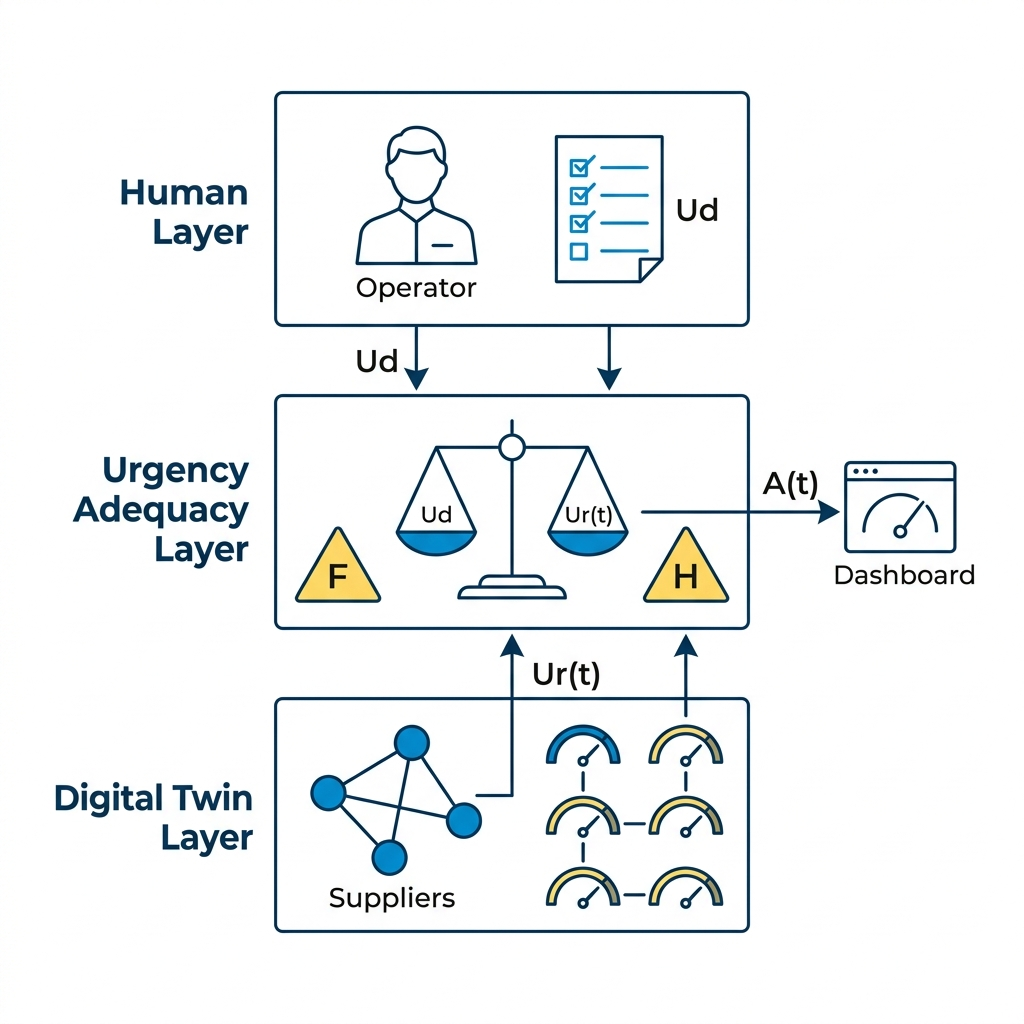
\includegraphics[width=0.85\linewidth]{Images/2.Problem/three_layer_architecture.png}
    \caption{The three-layer urgency adequacy architecture investigated in this work (Challenge~5).}
    \label{fig:todraw_threelayer}
\end{figure}


\clearpage
\section{State of the Art}
\label{sec:SOTA}
%% ═══════════════════════════════════════════════════════════════════════════
\subsection{Introduction: Key Definitions}
%% ═══════════════════════════════════════════════════════════════════════════

\textbf{Urgency} is defined here as the degree to which a supply chain task requires prompt action to avoid a material deterioration in operational performance. It differs from \emph{importance}, which reflects strategic value, and from \emph{priority}, which reflects the current execution order. In this work, urgency is treated as a multi-dimensional operational quantity, aggregated from heterogeneous KPI evidence rather than from a single deadline-driven signal~\autocite{cheng2025survey,zhu2018mere}.

\textbf{Real-time scheduling} refers to the class of algorithms that assign execution order to tasks given temporal constraints (deadlines, inter-task dependencies), resource constraints (vehicle capacity, supplier availability), and optimality criteria (makespan, weighted tardiness)~\autocite{pinedo2012scheduling}. This literature is drawn on here only as historical grounding for deadline-sensitive value functions; the present work does not deliver a scheduling algorithm.

\textbf{Digital twin} is a synchronized digital representation of a physical system that supports monitoring, simulation, and decision-making using real-time and historical data~\autocite{ivanov2020digital}. In supply chains, digital twins are used to improve visibility, disruption assessment, and replanning under changing conditions~\autocite{ivanov2020digital,ding2023realtime,hrusovsky2021realtime}.

\textbf{Multi-criteria decision-making (\gls{mcdm})} encompasses methods that combine multiple, potentially conflicting performance dimensions into a decision~\autocite{saaty1980analytic,brans1986promethee}. In the present work, the main dimensions considered for node prioritisation are time pressure, capacity saturation, operational performance, failure risk, cost drift, and carbon overshoot.

\textbf{Physical Internet} (\gls{pi}) is the paradigm of open, mutualized logistics networks that route shipments through shared infrastructure using standardised modular containers~\autocite{montreuil2011toward}. In such shared logistics environments, inaccurate urgency assessment may have effects beyond a single actor by influencing the allocation of mutualized capacity. This makes urgency evaluation particularly important in Physical Internet settings~\autocite{montreuil2011toward,leung2022digital}.

\textbf{Serious game} is a simulation environment designed to train decision-makers through realistic scenarios with immediate feedback and scoring~\autocite{sterman1989modeling,prensky2001digital}. In this project, DISCO functions both as a serious game and as a digital twin: users interact with simulated supply chain decisions, while the underlying digital model evaluates operational consequences on a weekly cadence.


%% ═══════════════════════════════════════════════════════════════════════════
\subsection{Literature Review}
%% ═══════════════════════════════════════════════════════════════════════════

The literature relevant to this framework is broad but fragmented. No retrieved work
in the project searches combines, within a single supply-chain decision
architecture, five elements at once: a multi-block operational urgency function, a
structured client-side urgency input, an adequacy layer comparing stated and
operational urgency, network propagation of that urgency across a multi-tier DAG, and
empirical validation of the adequacy signal against recorded
outcomes~\autocite{sawik2013integrated,sawik2014joint,sawik2016integrated,cohen2021assigning,hosseini2020bayesian}.

The review is organised by argumentative function. Two foundational streams establish
\emph{why} the problem exists. Two enabling streams provide the computational toolkit.
One section covers the closest antecedents. Analogical literature provides rhetorical
grounding but is labelled explicitly as non-foundational throughout.

Table~\ref{tab:stream_synthesis} summarises the seven streams and their relationship to
the thesis.

\begin{table}[H]
\centering
\caption{Literature stream synthesis: contribution and gap relative to this thesis.}
\label{tab:stream_synthesis}
\small
\begin{tabularx}{\linewidth}{>{\raggedright\arraybackslash}p{3.5cm} >{\raggedright\arraybackslash}p{2.2cm} >{\raggedright\arraybackslash}X >{\raggedright\arraybackslash}X}
\toprule
\textbf{Stream} & \textbf{Role} & \textbf{Main contribution} & \textbf{Gap relative to this thesis} \\
\midrule
Risk propagation and deadline-sensitive value & Foundation &
  Monotone time-value functions; ripple-effect propagation on networks &
  No declared-vs-operational comparison \\[3pt]
Cognitive bias in urgency & Foundation &
  Documents urgency mis-declaration patterns &
  No operational correction mechanism \\[3pt]
Digital twins of network risk and MCDM supplier scheduling & Closest antecedent &
  Multi-criteria supplier scoring and network disruption monitoring &
  No client-declared urgency or adequacy layer \\[3pt]
Bayesian and probabilistic risk updating & Enabling method &
  Conjugate/probabilistic belief revision under new evidence &
  Not used to compare declared vs.\ computed urgency \\[3pt]
Digital twin operations & Enabling method &
  Real-time replanning and disruption response &
  No stated-vs-operational urgency module found \\[3pt]
MCDM methods & Enabling method &
  Criteria weighting and outranking &
  Rank reversal risk; nominal weights $\neq$ effective weights \\[3pt]
Medical triage / PI / CO\textsubscript{2} & Analogy / Context &
  Asymmetric urgency vocabulary; network context &
  Analogical only (no formal transfer) \\
\bottomrule
\end{tabularx}
\end{table}

%% ───────────────────────────────────────────────────────────────────────
\subsubsection{Stream~1: Risk Propagation and Deadline-Sensitive Value}
\label{subsec:temporal}
%% ───────────────────────────────────────────────────────────────────────

\noindent\textit{Role: Foundation. \\ Why: It demonstrates that operational value can be formulated as a time-dependent and network-dependent quantity, providing the primary motivation for treating urgency as a variable that is both time-varying and propagated across a multi-tier network rather than computed at a single node in isolation.}

\medskip

Within real-time systems, deadline-sensitive scheduling theory models task value as a function of completion or response time, a paradigm known as time-value or utility-accrual scheduling~\autocite{cheng1996due,cheng2025survey}. Cheng and M\"uhlethaler~\autocite{cheng1996due} show that task utility is typically constant up to a deadline and then non-increasing with delay; the utility-accrual survey by Chen and Bella~\autocite{cheng2025survey} confirms that deadline-sensitive literature represents task value as a function of response time with bounded, structured degradation after critical thresholds. This establishes the historical precedent for treating urgency as time-varying, but it stops at a single task in isolation.

A second, complementary line of evidence comes from network risk-propagation research. Ivanov and colleagues formalise the ripple effect, whereby a local disruption at one supplier cascades through downstream tiers and amplifies as it travels along the network~\autocite{ivanov2020digital,ivanov2019viable,li2020exploring}. Probabilistic risk-inference methods for supply chain systems~\autocite{Zhe20} further show that aggregating heterogeneous risk indicators into a single node-level score is itself an open modelling question, distinct from how that score should then be propagated.

Table~\ref{tab:urgency_models} compares four candidate aggregation and growth models found across these two lines of literature.

\begin{table}[H]
\centering
\caption{Comparative urgency aggregation and growth models and their properties.}
\label{tab:urgency_models}
\small
\begin{tabularx}{\linewidth}{>{\raggedright\arraybackslash}p{2.6cm} >{\raggedright\arraybackslash}p{2.6cm} >{\raggedright\arraybackslash}X >{\raggedright\arraybackslash}p{2.4cm}}
\toprule
\textbf{Model} & \textbf{Formula} & \textbf{Key property} & \textbf{Use case} \\
\midrule
Linear (time) & $U_0 + \lambda t$ & Constant pressure & Administrative tasks \\[3pt]
Hyperbolic (time) & $K / (t_c - t)$, bounded via $\tanh$ & Finite-time singularity, discounting & Synthetic scenario generation \\[3pt]
Weighted average (blocks) & $\sum_m \omega_m u_m$ & Fully compensatory: one weak block hidden by strong ones & Simple composite indices \\[3pt]
Noisy-OR (blocks) & $1-\prod_m(1-u_m)^{\omega_m}$ & Non-compensatory: one saturated block dominates & Multi-block operational risk \\
\bottomrule
\end{tabularx}
\end{table}

This thesis adopts the noisy-OR aggregation over the fully compensatory weighted average, on the grounds that a single catastrophic KPI block (for instance a complete capacity failure) should not be masked by acceptable scores on the remaining blocks, a property established in the probabilistic-inference literature on combining independent causal evidence~\autocite{pearl1988probabilistic}. The bounded hyperbolic discounting curve is retained separately, purely as an auxiliary tool for generating realistic synthetic urgency trajectories used in testing and calibration; a structurally similar acceleration appears in Log-Periodic Power Law (\gls{lppl}) models of financial crash precursors~\autocite{johansen2001finite,johansen2000crashes}, used here strictly as an analogical reference for that auxiliary generator, since empirical analyses by Feigenbaum~\autocite{feigenbaum2001statistical} and Br{\'e}e et al.~\autocite{bree2010prediction} show that LPPL-family models are highly parameter-sensitive and unsuited to direct use as a production risk model.

\medskip
\noindent\textbf{Summary of Stream~1:}
\begin{itemize}
    \item \textbf{Established literature:} Deadline-sensitive scheduling supports time-dependent task valuation~\autocite{cheng2025survey}; ripple-effect research supports network propagation of local disruptions~\autocite{ivanov2020digital,li2020exploring}.
    \item \textbf{Research gap:} Neither stream specifies how to aggregate heterogeneous, block-structured operational risk indicators at a single node before propagating them.
    \item \textbf{Working assumption:} A non-compensatory, noisy-OR aggregation of KPI blocks is proposed as the local urgency model, to be propagated with a leaky product rule across the network.
    \item \textbf{Systemic gap:} While these streams model network propagation and deadline sensitivity, neither addresses user-declared urgency or the mismatch between stated and operational urgency.
\end{itemize}
%% ───────────────────────────────────────────────────────────────────────
\subsubsection{Stream~2: Cognitive Bias in Urgency Declaration}
\label{subsec:biases}
%% ───────────────────────────────────────────────────────────────────────

\noindent\textit{Role: Foundation. \\ Why: It establishes that client-declared urgency is
systematically biased and cannot be taken at face value as a planning input.}

\medskip

Behavioural operations research suggests that human decision-makers systematically
misrepresent urgency, a finding with direct implications for any system that relies on
operator-declared urgency as an input.

Two convergent lines show this from different angles. Zhu, Yang and
Hsee~\autocite{zhu2018mere} report the Mere-Urgency Effect in five controlled experiments:
participants consistently over-prioritised imminent low-value tasks over distant
high-value tasks, and the bias persisted even when participants were informed of its
existence. Steel~\autocite{steel2006integrating} provides a complementary formal model
through Temporal Motivational Theory (\gls{tmt}):
\begin{equation}
    V(t) = \frac{U \cdot E}{1 + \Gamma \cdot D(t)^k},
    \label{eq:tmt_val}
\end{equation}
where $U$ is objective utility, $E$ is the expectancy of success, $D(t)$ is the delay
to deadline, and $\Gamma$, $k$ are individual discounting parameters. As $D(t) \to 0$,
$V(t) \to U \cdot E$, so immediacy becomes more salient as the deadline approaches.
Near-term tasks can therefore attract disproportionate attention even when their broader
objective value is lower~\autocite{steel2006integrating}, which helps explain why
imminent tasks may be over-declared as urgent. The operational roles of the parameters in this formulation are structured in Table~\ref{tab:tmt_vars}.

\begin{table}[H]
\centering
\caption{Temporal Motivational Theory (TMT) parameters and domains.}
\label{tab:tmt_vars}
\begin{tabularx}{\linewidth}{llX}
\toprule
\textbf{Symbol} & \textbf{Concept} & \textbf{Operational Role} \\
\midrule
$V(t)$ & Temporal motivational value & Dynamic task salience \\
$U$ & Objective utility & Task strategic importance \\
$E$ & Expectancy of success & Probability of task completion \\
$D(t)$ & Delay to deadline & Remaining safe execution window \\
$\Gamma$ & Impulsiveness parameter & Operator sensitivity to delay \\
$k$ & Sensitivity scaling parameter & Non-linear scaling of delay discounting \\
\bottomrule
\end{tabularx}
\end{table}

These laboratory findings are supported by evidence from operational settings.
Rusou, Amar and Ayal~\autocite{rusou2020psychology} show that operators under workload
preferentially complete small, easy tasks, the operational analogue of under-triage for
large-scope supply chain activities. DiwasSingh et al.~\autocite{diwa2020task} confirm
in a large field study that completing easy tasks first significantly hurts overall
performance. Hospital admission control under occupancy uncertainty~\autocite{kim2020admission}
produces over- and under-triage patterns analogous to those in logistics operator
decisions under uncertain lead times. The magnitude of these biases in industrial supply chain contexts remains a subject of calibration. To mitigate these time-perception and workload biases, human-centered decision support systems (such as Rosenthal and Hiatt~\autocite{rosenthal2020human}) use visual feedback techniques to show the mismatch between human plans and system temporal constraints, helping users calibrate their schedules.

This study treats declared urgency as a noisy signal and computes a model-based
correction. The correction mechanism, and its empirical predictive validity, is detailed in Section~\ref{sec:Operations}.

\medskip
\noindent\textbf{Summary.} \\
\textit{Known}: Urgency over-declaration for near-deadline tasks is documented in
controlled settings~\autocite{zhu2018mere} and in operational
settings~\autocite{diwa2020task,rusou2020psychology}. \\
\textit{Unknown}: Bias magnitude in industrial supply chain contexts. \\
\textit{Assumed}: Asymmetric penalty $\lambda_{\text{under}} > \lambda_{\text{over}}$
is the appropriate correction structure. \\
\textit{Open gap}: Behavioural research diagnoses the problem. It does not prescribe a
real-time operational correction.

%% ───────────────────────────────────────────────────────────────────────
\subsubsection{Closest Antecedents: Digital Twins of Network Risk and MCDM Supplier Scoring}
\label{subsec:antecedents}
%% ───────────────────────────────────────────────────────────────────────

\noindent\textit{Role: Closest antecedents. \\ Why: These are the works most structurally
similar to the thesis. Identifying their gap precisely isolates what this work adds.}

\medskip

The works most structurally similar to this thesis combine multi-criteria supplier
scoring with disruption-aware network monitoring.
Sawik~\autocite{sawik2013integrated,sawik2014joint,sawik2016integrated} develops
mixed-integer programming models for resilient supplier order assignment integrating
cost, service level, and disruption risk. Cohen and Kaspi~\autocite{cohen2021assigning}
and Afrasiabi et al.~\autocite{afrasiabi2022extended} extend this to \gls{mcdm}
supplier prioritisation under disruption, combining criteria weighting with allocation
optimisation. Chakrabortty et al.~\autocite{chakrabortty2020efficient} confirm that
rule-based heuristics remain competitive against exact methods in dynamic
industrial environments. These works are cited here for the closeness of their subject
matter (multi-criteria, disruption-aware supply chain decisions), not because this
thesis reuses their optimisation machinery, which addresses allocation and sequencing
rather than urgency measurement.

Taken together, this stream models disruption-aware supplier evaluation with
multi-criteria weighting. Two gaps distinguish it from the present work. First, none
introduces a network-propagated urgency signal computed independently at every node
and combined across tiers; risk is typically evaluated once, at the point of decision.
Second, none compares a client-stated urgency against a model-derived urgency: the
client-declared signal, where it exists, is used directly, without validation against
live operational proxies.

\medskip
\noindent\textbf{Narrow gap statement.}
In the retrieved literature, no work simultaneously (i)~aggregates heterogeneous
operational risk into a multi-block urgency function propagated across a DAG,
(ii)~captures client-declared urgency as a structured, consistency-gated input, and
(iii)~feeds the mismatch between (i) and (ii) into an empirically calibrated
adequacy score. Each stream addresses at most two of these three requirements.

\medskip
\noindent\textbf{Commercial positioning.} The same gap was checked informally against commercial multi-tier supply chain risk-monitoring platforms (for example Everstream Analytics, Resilinc, and Interos), which map supplier networks to several tiers and continuously score them against pre-defined disruption scenarios. This is an informal product review rather than an academic source, and is stated here as the project's own positioning assessment: to the team's knowledge, none of these platforms compares a client-declared urgency signal against their own computed risk score, which is the specific mismatch this framework targets.

%% ───────────────────────────────────────────────────────────────────────
\subsubsection{Enabling Method: Bayesian and Probabilistic Risk Updating}
\label{subsec:bayesian}
%% ───────────────────────────────────────────────────────────────────────

\noindent\textit{Role: Enabling method. \\ Why: Revising a failure probability from a
small number of new observations is a component of operational risk state. Bayesian
conjugate updating is the borrowed tool.}

\medskip

Bayesian methods have emerged as a well-supported approach for revising risk estimates
from new evidence in supply chain research~\autocite{pearl1988probabilistic,koller2009probabilistic}. Rather than a full Bayesian network with an explicit
conditional-probability-table structure, this study draws on the narrower and more
tractable case of Beta-Bernoulli conjugate updating: a failure probability
$p$ is treated as a Beta-distributed belief with an equivalent prior sample size
$n_0$, revised from a small number of newly observed equivalent trials
$(k, n)$ each time a calibrated operational event is declared. This is the
standard conjugate-prior construction for binomial-outcome belief
revision~\autocite{pearl1988probabilistic,koller2009probabilistic}.

Three convergent findings from the retrieved Bayesian supply-chain literature support
this choice of tool. Hosseini and Ivanov~\autocite{hosseini2020bayesian} provide the most
comprehensive survey (259~citations) of Bayesian methods applied to supply chain risk and
resilience, finding that probabilistic belief-revision methods are often preferred to
simple deterministic scoring when new, sparse evidence must update an existing risk
estimate. Huang et al.~\autocite{huang2020bayesian} and Deng, Zhang and
Wei~\autocite{deng2020prediction} develop Bayesian models for disruption and delay
probability estimation that serve as a methodological precedent for revising a KPI
block's failure probability from a declared event. Lockamy~\autocite{lockamy2011bayesian} and
Qazi et al.~\autocite{qazi2017dynamic} further support Bayesian revision as a practical
tool for dynamic supply chain risk quantification under sparse, event-driven evidence,
consistent with the small-sample setting of a weekly-cadence digital twin. Plain
frequency counts, by contrast, are unstable when only a handful of events are declared
per node per project, which motivates the conjugate-prior formulation adopted here
over a raw frequentist estimate~\autocite{zheng2020risk}.

The specific conjugate-update parameters used for each event family are developed in
Section~\ref{sec:Operations}.

\medskip
\noindent\textbf{Summary.} \\
\textit{Known}: Bayesian conjugate updating is an established, low-data-regime tool for
revising failure probabilities in logistics contexts. \\
\textit{Unknown}: The optimal prior sample size for DISCO's specific event taxonomy. \\
\textit{Assumed}: A shared, moderately informative prior (equivalent to roughly
six months of weekly observations) is sufficient for initial calibration. \\
\textit{Open gap}: Bayesian belief revision quantifies disruption exposure but does not,
by itself, compare it against client-declared urgency.

%% ───────────────────────────────────────────────────────────────────────
\subsubsection{Enabling Method: Digital Twin and Real-Time Decision Support}
\label{subsec:dt}
%% ───────────────────────────────────────────────────────────────────────

\noindent\textit{Role: Enabling method and primary gap source. \\ Why: DT systems are the
architectural family closest to DISCO; this review establishes both what they already do
and the specific gap this thesis addresses.}

\medskip

The digital twin concept was formalised by Grieves~\autocite{grieves2014digital} as a
virtualised representation of a physical process. Tao et al.~\autocite{tao2018digital}
extended the concept to manufacturing; Fuller et al.~\autocite{fuller2020digital}
surveyed the enabling technologies underpinning modern deployments. In supply chain
management, Ivanov et al.~\autocite{ivanov2021digital} define the \gls{sc} \gls{dt} as
integrating simulation (what-if analysis), optimisation (decision support), and machine
learning (pattern detection). Ivanov and Dolgui~\autocite{ivanov2020digital} address the
use of digital \gls{sc} twins for disruption risk and resilience management in the
Industry~4.0 era. Wang, Wang and Liu~\autocite{wang2020digital} demonstrate
\gls{dt}-driven planning in a manufacturing context analogous to DISCO's satellite
component network. More recently, in the context of Industry 5.0, these systems have evolved towards Human-in-the-Loop (HITL) Cognitive Digital Twins (CDTs) where semantic models and reasoning methods are used to capture human feedback and synchronize mental models with simulated physical operations~\autocite{niloofar2023}.

Real-time freight planning work demonstrates that operational urgency proxies (slack, lateness risk, and shortage exposure) are present within these
systems~\autocite{hrusovsky2021realtime,perez2022digital}. Model-predictive control
approaches for vehicle routing~\autocite{karam2022realtime} and digital-twin disruption
response~\autocite{ding2023realtime,leung2022digital,zhu2025industry5} confirm the
state of the art in live operational replanning.

Taken together, the digital-twin literature supports simulation, optimisation, and
disruption-aware decision support. In the retrieved literature, however, no system surfaces a standard module that:
\begin{itemize}
    \item captures a client-declared urgency signal as a structured input,
    \item computes a model-based operational urgency from the live system state, and
    \item measures their mismatch as an active, network-propagated indicator.
\end{itemize}
This three-layer architecture appears to be an open slot in digital \gls{sc} operations (stated as an observation from the retrieved literature, not as a claim about the totality of published work). Whether filling this gap improves the identification of at-risk nodes is the central empirical hypothesis
of this thesis (Lock~3, Section~\ref{sec:locks}).

\subsubsection{Enabling Methods: Multi-Criteria Decision Methods}
\label{subsec:mcdm}
%% ───────────────────────────────────────────────────────────────────────

\noindent\textit{Role: Enabling methods. \\ Why: These multi-criteria decision-making (\gls{mcdm}) tools provide the computational foundation for criteria weighting, outranking, and network prioritisation.}

\medskip

This research integrates and builds upon two distinct methodological domains within multi-criteria decision-making: pairwise comparison methods for eliciting weights, and outranking aggregation for turning those weights into a defensible ranking of nodes.

\paragraph{Pairwise Elicitation and Pairwise Comparison Methods.}
To construct a structured representation of operator-declared urgency ($U_d$), criteria weights must be systematically elicited. The Analytic Hierarchy Process (\gls{ahp})~\autocite{saaty1980analytic} derives criteria weights as the principal eigenvector of a pairwise comparison matrix, validating logical consistency via the Consistency Ratio ($\gls{cr} \le 0.10$). While widely applied in logistics, AHP suffers from rank reversal, where the introduction of a new alternative alters the relative ranking of existing ones, and is sensitive to cognitive noise during expert elicitation~\autocite{dyer1990,triantaphyllou2024}.

To minimize operator cognitive load and improve consistency, the Best-Worst Method (\gls{bwm})~\autocite{rezaei2015best} reduces the number of required pairwise comparisons from $n(n-1)/2$ to $2(n-1)$ by anchoring comparisons around chosen "best" and "worst" criteria. This is further extended by the Fuzzy Best-Worst Method (\gls{fbwm})~\autocite{guo2017fuzzy,Yuc18,amiri2020new}, which uses Triangular Fuzzy Numbers (\glspl{tfn}) to absorb human judgment uncertainty. In this study, consistent FBWM weight vectors~\autocite{liang2020} serve as an alternative elicitation gate to crisp AHP, and both feed the same downstream propagation and adequacy machinery.

\paragraph{Outranking Aggregation, Network Criticality, and Composite Indicator Critique.}
For prioritising which nodes require attention, direct weighted averages risk full compensatory aggregation, where an excellent score on one criterion (e.g., cost) completely masks a critical failure on another (e.g., capacity). To prevent this, outranking methods such as PROMETHEE~II~\autocite{brans1986promethee,brans2005promethee} establish pairwise preference flows ($\phi^+$ and $\phi^-$), allowing a non-compensatory ordering of alternatives. A comprehensive survey of PROMETHEE applications~\autocite{behzadian2010promethee} confirms its suitability for supplier and node evaluation in industrial contexts. In this work, PROMETHEE~II ranks active network nodes directly on the same weighted KPI blocks that feed the local urgency aggregation, giving a network-wide outranking view that complements the per-node adequacy score. Systematic what-if shock simulation, in which a node's local risk is forced to saturation and the resulting propagated delta is measured across the network, provides a second, independent criticality signal that is combined with the outranking flow to identify structural bottlenecks.

However, constructing any composite indicator from weighted criteria introduces methodological challenges. Composite-index literature warns that nominal weights assigned to criteria often diverge from their effective importance due to correlation, normalization, and aggregation dynamics~\autocite{greco2018,becker2017,borgonovo2021global}. Furthermore, the choice of normalization method is non-neutral and can lead to rank reversal~\autocite{triantaphyllou2000multi}. To keep the aggregation weights interpretable and defensible, this study exposes per-block contributions on the operator explainability page rather than only the aggregate score, while validating the risk parameters under uncertainty~\autocite{sawik2020risk}.

\subsubsection{Analogical and Contextual Literature}
\label{subsec:triage}
%% ───────────────────────────────────────────────────────────────────────

\noindent\textit{Role: Analogies and context. \\ Why: These bodies of literature provide conceptual analogies (medical triage), network contexts (Physical Internet), or regulatory frameworks (carbon accounting) that support the design of the adequacy variables.}

\medskip

While the core scoring and network-propagation methods are mathematically derived, their operational structure draws grounding and context from three non-foundational literature streams.

\paragraph{Medical Triage as a Conceptual Analogy.}
Medical triage provides a rich conceptual analogy for prioritizing tasks under severe capacity constraints and cognitive pressure. Standard protocols such as the Manchester Triage System (\gls{mts})~\autocite{mackway2013emergency} categorize patients into five urgency levels using flowcharts, whereas the Emergency Severity Index (ESI) integrates predicted resource consumption. Comparative clinical studies~\autocite{kuligowski2025comparative} show significant classification discrepancies (weighted $\kappa = 0.51$) between these systems, highlighting that even trained professionals struggle with consistent urgency assessment.

In a supply chain context, this triage process maps directly to node prioritisation. The design of the cognitive adequacy score $A(t)$ is motivated by the clinical principle of asymmetric risk: under-triage (under-declaring urgency, leading to untreated critical conditions) is far more dangerous than over-triage (over-declaring urgency, leading to resource congestion)~\autocite{kim2020admission}. Consequently, the adequacy score enforces an asymmetric penalty ($\lambda_{\text{under}} > \lambda_{\text{over}}$) to protect the physical supply chain from hidden stockout ruptures. Table~\ref{tab:triage_transfer} maps these triage concepts to their logistics equivalents.

\begin{table}[H]
\centering
\caption{Heuristic mapping of medical triage concepts to DISCO logistics prioritisation.}
\label{tab:triage_transfer}
\begin{tabularx}{\linewidth}{lX}
\toprule
\textbf{Medical concept} & \textbf{DISCO logistics equivalent} \\
\midrule
Patient priority P1 (immediate) & Node with $A(t) < 20$ and high network criticality rank \\
Under-triage (P3 classified as P1) & Hidden risk $H = [U_r - U_d]_+$: silent bottleneck builds unnoticed \\
ESI resource consumption estimate & DISCO criticality index (propagated impact on final-customer nodes) \\
Resource-blind triage (MTS) & Local urgency threshold ignoring network position \\
Resource-aware triage (ESI) & Criticality-weighted prioritisation of coordinator attention \\
\bottomrule
\end{tabularx}
\end{table}
\paragraph{Physical Internet and Supply Chain Synchromodality.}
The Physical Internet (\gls{pi}) paradigm~\autocite{montreuil2011toward} conceptualizes open, mutualized logistics networks where routing, storage, and transport assets are shared. In such hyperconnected systems, urgency ceases to be a localized concern and becomes a network-level Quality of Service variable. Dynamic routing and order synchronization in synchromodal networks require real-time, responsive priority signals compatible with rolling planning windows~\autocite{guo2020dynamic}. Furthermore, disruptions propagate rapidly through hyperconnected networks, creating cascading ripple effects~\autocite{li2020exploring} that validate the need for a synchronized, digital-twin-driven propagation model~\autocite{ivanov2020digital}.

\paragraph{Regulatory Carbon Accounting.}
The integration of an environmental criterion is motivated by modern corporate sustainability requirements, such as the Corporate Sustainability Reporting Directive (CSRD Scope 3) and ALTEN's environmental guidelines~\autocite{cordova2024green}. Standardized frameworks like the \gls{glec} Framework v3.2~\autocite{smartfreight2023glec} and \gls{vecto}~\autocite{commission2017vecto} define emissions calculation baselines for heavy duty vehicles. ADEME~\autocite{ademe2014impacts} reports that emissions factors are non-linearly related to vehicle speed and cargo load, supporting the treatment of carbon overshoot as its own urgency block rather than folding it into a generic cost term.

%% ───────────────────────────────────────────────────────────────────────
\subsubsection{Validation Methodology: Serious Games}
\label{subsec:games}
%% ───────────────────────────────────────────────────────────────────────

\noindent\textit{Role: Validation rationale. \\ Why: It justifies the weekly-cadence serious game
used as the validation environment for the whole framework.}

\medskip

The Beer Game~\autocite{sterman1989modeling} is the foundational supply chain serious game: Sterman demonstrates that players systematically under-react to upstream demand signals, generating the bullwhip effect. This decision bias is analogous to the under-triage pathology in logistics, where operators consistently under-respond to signals of building urgency. The finding that game-based observation captures systematic decision biases supports the use of digital twin serious games as an empirical instrument. Prensky~\autocite{prensky2001digital} establishes the theoretical basis for digital game-based learning, and Deterding et al.~\autocite{deterding2011game} formalise gamification design principles.

Mohaddesi et al.~\autocite{mohaddesi2020gamettes} introduce the Gamette methodology, a playful, bite-sized approach to capturing decision-making patterns to build behavioural models, directly applicable to a weekly-review protocol in which operators repeatedly submit urgency assessments over the course of a project. Bellotti et al.~\autocite{bellotti2013framework} provide an evaluation framework for serious game learning outcomes, which supports the design of the calibration methodology detailed in Section~\ref{sec:Operations}.


%% ═══════════════════════════════════════════════════════════════════════════
\subsection{Summary: Limitations of Existing Solutions}
\label{subsec:gaps}
%% ═══════════════════════════════════════════════════════════════════════════

A review of the literature indicates that classical operational monitoring typically evaluates a single criterion (a deadline, a cost, or a risk score) at a time, failing to capture the multi-block nature of supply chain KPIs or the systemic impact of operator decision biases. While pairwise comparison methods (AHP, BWM, and Fuzzy BWM) are widely applied for criteria weighting, they function as static elicitation tools and are rarely compared against a computed operational counterpart. Outranking methods like PROMETHEE II prevent compensatory aggregation but are not usually combined with a network-propagated urgency signal.

Furthermore, while contemporary supply chain digital twins and Bayesian risk models offer strong capabilities in real-time disruption monitoring and belief revision, they typically lack a mechanism to compare human operator inputs with the physical state of the digital twin. This review identifies a key gap: the absence of an integrated architecture that compares a declared client-side urgency signal against a computed, network-propagated operational urgency to evaluate and correct cognitive mismatch, and that validates this correction empirically against recorded operational outcomes. Whether this adequacy-driven prioritisation improves the identification of at-risk nodes compared to standard KPI baselines represents the central open question of this R\&D operation.

%% ═══════════════════════════════════════════════════════════════════════════
\subsection{Research Axis and Proposed Adequacy-Propagation Structure}
\label{subsec:contribution}
%% ═══════════════════════════════════════════════════════════════════════════

To investigate this gap, this study proposes an architecture centered on a cognitive-physical adequacy check combined with network-wide risk propagation. The main objective is to design and evaluate a two-layer control loop:
\begin{enumerate}
    \item \textbf{Cognitive adequacy check}: This layer captures the operator's declared urgency $U_d$ (elicited through consistency-gated pairwise comparisons) and compares it with a physically-grounded real urgency $U_r(t)$ computed from live digital twin state. The mismatch is processed using an asymmetric penalty to debias operator judgments.
    \item \textbf{Network propagation and criticality-driven prioritisation}: Local urgency is propagated across the supply chain DAG (declared urgency descending toward suppliers, real urgency ascending toward the final customer), and the resulting network state feeds both a PROMETHEE~II outranking ranking and a systematic shock-simulation criticality index, jointly identifying which nodes warrant prioritised operator attention.
\end{enumerate}

This two-layer architecture is exercised and empirically validated within a persistent, multi-tenant digital twin operated as a weekly-cadence serious game, closing the loop between the adequacy signal and observed operational outcomes (Section~\ref{sec:Operations}).


\clearpage
\section{Conducted Operations}
\label{sec:Operations}
%% ═══════════════════════════════════════════════════════════════════════════
\subsection{Methodology: The Agile Test-and-Learn Program}
%% ═══════════════════════════════════════════════════════════════════════════

This R\&D operation is structured as an agile Test-and-Learn program designed to investigate cognitive biases in supply chain urgency assessment and formulate a digital-twin-based correction loop. Rather than following a rigid sequential path, the program operates through continuous iterations of literature analysis, mathematical specification, software implementation, and scenario-based simulation.

The R\&D pipeline is organized into four core operational areas:
\begin{itemize}
    \item \textbf{Literature Review and Gap Analysis}: Establishing the psychological and mathematical foundations of multi-block urgency aggregation and cognitive bias (detailed in Section~\ref{sec:SOTA}).
    \item \textbf{Mathematical Framework Specification}: Deriving and formalizing the multi-block real urgency function, its DAG propagation, and the asymmetric cognitive adequacy score from first principles to ensure dimensional and probabilistic consistency.
    \item \textbf{Pairwise comparison elicitation}: Formulating crisp Analytic Hierarchy Process (AHP) and Fuzzy Best-Worst Method (F-BWM) eigenvectors to build a reliable representation of declared operator urgency.
    \item \textbf{Implementation, Simulation and Validation}: Building a modular, tested Python library (73 modules, 1\,831 automated test functions expanding to 2\,044 collected cases) exercised through a multi-page Dash web application, running controlled shock and scenario simulations on a persistent digital twin, and confronting the hidden-risk signal with recorded outcomes through a dedicated calibration service and a serious-game campaign (Section~\ref{sec:serious_game}).
\end{itemize}

The remainder of this section follows that same separation explicitly: the mathematical model is presented on its own (Section~\ref{sec:math_framework}), independently of how it is elicited, computed, and exposed (Section~\ref{sec:application}), before turning to the use case built to validate it (Section~\ref{sec:serious_game}).

\begin{figure}[H]
    \centering
    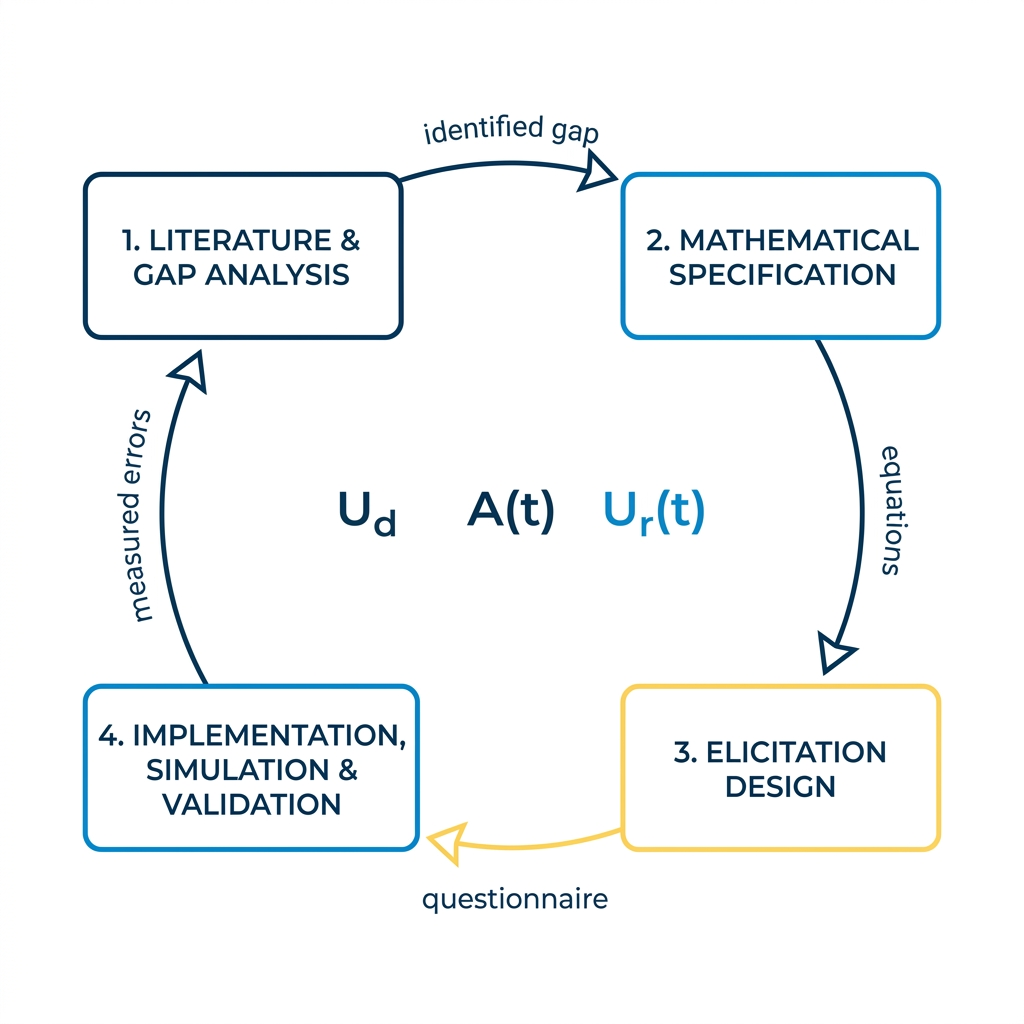
\includegraphics[width=0.85\linewidth]{Images/4.Operations/test_learn_loop.png}
    \caption{The agile Test-and-Learn iteration loop of the R\&D operation.}
    \label{fig:todraw_loop}
\end{figure}

%% ═══════════════════════════════════════════════════════════════════════════
\subsection{Mathematical Model}
\label{sec:math_framework}
%% ═══════════════════════════════════════════════════════════════════════════

This section states the model on its own terms: what real urgency and declared urgency are, how each is propagated across the network, and how their mismatch is scored. It intentionally leaves out tooling and interface choices, elicitation mechanics, and operational cadence, which are application decisions addressed separately in Section~\ref{sec:application}.

\subsubsection{Core Model: Real and Declared Local Urgency, and Network Propagation}

\paragraph{Local Real Urgency ($U_{r,\text{local}}$).}
Real urgency is not read from a single deadline-proximity signal; it is aggregated at each node from six independent KPI blocks, $\{\text{time}, \text{cap}, \text{perf}, \text{risk}, \text{cost}, \text{co2}\}$, each producing a partial urgency $u_m \in [0,1]$ or \texttt{None} when the underlying KPI data is unavailable. The aggregation is a weighted probabilistic OR, so that a single saturated block is sufficient to drive the local urgency toward its maximum, regardless of how well the other blocks score:
\begin{equation}
    U_{r,\text{local}} = 1 - \prod_{m} (1 - u_m)^{\omega_m},
    \label{eq:ur_local}
\end{equation}
where $\omega_m \ge 0$ is the aggregation weight of block $m$, and the product runs over blocks with available data. Table~\ref{tab:ur_blocks} gives, for each block, its schematic formula and what it measures; the notation $[x]_+ = \max(x, 0)$ denotes the positive part, and the per-term weights ($\alpha_i$, $\beta_i$) are renormalised over the terms whose data is actually available.

\begin{table}[H]
\centering
\caption{The six real urgency blocks: formula and explanation.}
\label{tab:ur_blocks}
\small
\begin{tabularx}{\linewidth}{l >{\raggedright\arraybackslash}p{4.6cm} X}
\toprule
\textbf{Block} & \textbf{Formula} & \textbf{Explanation} \\
\midrule
$u_{\text{time}}$ & $P(L > d^\ast - t) + \kappa_{\text{retard}}[r]_+ - \kappa_{\text{avance}}[-r]_+$ & Probability that the lead time $L$, modelled as Normal($\mu$, $\sigma$), exceeds the time left before the next active deadline $d^\ast$; forced to $1$ once the deadline is passed. The planning term $r$ compares theoretical progress with reported progress: a milestone behind plan raises the block, one ahead of plan lowers it. \\
\midrule
$u_{\text{cap}}$ & $\alpha_1\bigl(1-\tfrac{V_{\text{rem}}}{V_{\max}}\bigr) + \alpha_2\bigl(1-\tfrac{W_{\text{rem}}}{W_{\max}}\bigr) + \alpha_3\bigl[\tfrac{D-\Phi}{D}\bigr]_+$ & Saturation of the node's capacity: how little storage volume and weight remain, plus the fraction of demand $D$ not covered by the current flow rate $\Phi$. \\
\midrule
$u_{\text{perf}}$ & $1 - \text{OEE}$ & Complement of Overall Equipment Effectiveness (availability $\times$ performance $\times$ quality): the lower the productive health of the critical resource, the higher the urgency. \\
\midrule
$u_{\text{risk}}$ & $1-\exp\bigl(-p_{\text{fail}} \times t_{\text{recov}} \times \text{sev}/T_{\text{ref}}\bigr)$ & Expected unavailability: failure probability times recovery time times impact severity, normalised by a reference horizon $T_{\text{ref}}$, then combined by probabilistic OR with the environmental and political exposure terms. \\
\midrule
$u_{\text{cost}}$ & $\beta_1\,\tfrac{c_{\text{op}}-c_{\text{nom}}}{c_{\text{nom}}} + \beta_2\,[\text{tariff}-1]_+ + \beta_3\,\tfrac{c_{\text{stock}}}{C_{\text{ref}}}$ & Financial stress: drift of operating cost above its nominal value, tariff multiplier above neutral, and storage cost relative to a reference cost. \\
\midrule
$u_{\text{co2}}$ & $\bigl[\tfrac{e - e_{\text{target}}}{e_{\max}-e_{\text{target}}}\bigr]_+$ & Normalised overshoot of measured emissions $e$ above the target, saturating at the maximum threshold. \\
\bottomrule
\end{tabularx}
\end{table}

% -----------------------------------------------------------------------------
% REMARQUE MÉTHODOLOGIQUE DÉTAILLÉE : FONCTIONS DE TRANSFERT ET NORMALISATION ADIMENSIONNELLE
% -----------------------------------------------------------------------------
% Pour répondre à la question du jury/examinateur ("Comment comparer des jours, des € et des % sans soustraire des pommes et du tissu ?") :
% 1. Chaque KPI physique brut (avec dimension : jours, €, kg, %) passe par une fonction de transfert u_m(·).
% 2. u_m(·) est une application mesurable de R_physique -> [0, 1] adimensionnel :
%    - u_m = 0.0 : état nominal / sérénité opérationnelle (aucun risque).
%    - u_m = 1.0 : saturation du bloc / rupture imminente ou consommée.
% 3. C'est ce rebasage adimensionnel strict sur [0, 1] qui rend légitime l'agrégation par Noisy-OR (Eq. 1)
%    et la confrontation asymétrique avec l'urgence déclarée U_d (élicitée par AHP sur [0, 1])
%    dans l'équation d'adéquation A(t) = 100 * (1 - Pénalité(U_d - U_r)).
% -----------------------------------------------------------------------------

Two conventions make this aggregation unambiguous, since a bare formula does not by itself say what its bounds mean. First, each $u_m$ is engineered to carry the same meaning regardless of which raw KPI feeds it: $u_m \to 0$ means the block is healthy and contributes no urgency, $u_m \to 1$ means the block is saturated, that is, it has reached the point past which it cannot make the node any more urgent, whether that point is a missed deadline, a fully depleted buffer, or a near-certain failure. This use of ``saturated'' is a design choice made for this model, not a term imported as-is from the literature; it is what makes the noisy-OR product in Equation~\ref{eq:ur_local} valid across six structurally different blocks, since the product only requires each factor to share the same $[0,1]$ urgency scale, not the same physical units or the same statistical behaviour between $0$ and $1$. Second, a block whose data is \texttt{None} is excluded from the product entirely rather than assigned a value: because the product runs only over blocks with available data, a missing block neither raises nor lowers $U_{r,\text{local}}$, it is simply absent from the evidence, and the remaining weights are renormalised over what is left. Treating the six blocks as comparable on $[0,1]$ is therefore a modelling commitment, not a measured property, and Section~\ref{sec:limitations} lists it among the framework's stated limitations.

Two lifecycle status rules are applied before aggregation: a node marked \texttt{DONE} has its effective local $U_r$ forced to $0.0$ (a completed task carries no further physical risk), while a node marked \texttt{ABANDONED} has it forced to $1.0$ (complete failure). These rules are applied identically whether the local urgency comes from the analytic blocks above or from the Monte Carlo estimate of the time block described below.

\paragraph{Why These Six Blocks: A Rupture-Risk-Driven Selection.}
The six blocks were not chosen as an arbitrary KPI shortlist. The selection started from the question that defines urgency in a supply chain: \emph{what mechanisms make the risk of a delivery rupture rise?} A rupture, that is the inability to deliver at the agreed time, place, quantity, and quality, is the terminal event the urgency signal must anticipate~\autocite{heckmann2015critical}. Working backwards from that event, and consistently with indicator-based supply risk monitoring~\autocite{mokhtar2019supplier}, four \emph{direct causal mechanisms} and two \emph{arbitration variables} were identified:

\begin{itemize}
    \item \textbf{Time erosion ($u_{\text{time}}$)}: the remaining slack between deadline and realistic lead time. Time is the only non-compressible resource: whatever the state of the other indicators, a task whose slack reaches zero can no longer be saved, which makes deadline proximity the variable most directly tied to operational urgency~\autocite{cohen2021assigning,bojarski2021,sun2020combating,sawik2013integrated}.
    \item \textbf{System saturation ($u_{\text{cap}}$)}: queues, transport capacity, workshop load, and bottlenecks. A saturated system introduces hidden waiting delays on top of the nominal lead time, so capacity stress raises non-delivery risk even when the announced lead time looks safe~\autocite{tomlin2006value,hosseini2019resilient,taghavi2024sustainable}.
    \item \textbf{Critical-resource performance ($u_{\text{perf}}$)}: drift in the performance of the resource that produces the part. OEE is used as a composite proxy (availability $\times$ performance $\times$ quality) rather than a single machine metric, because precise performance data is rarely accessible on the supplier side~\autocite{mokhtar2019supplier,hlioui2017joint}.
    \item \textbf{Adverse-event exposure ($u_{\text{risk}}$)}: the expectation of unavailability caused by a disruption, computed as failure probability $\times$ recovery time $\times$ impact severity, composed with environmental and political exposure. The default incident probability (0.02) is revised weekly from declared events through the Bayesian operator of Section~\ref{sec:weekly_cycle} over a $n_0 = 26$ iteration window; this block builds on the DIN supplier risk scorer~\autocite{kabouche2025scoring} and on probabilistic ripple-effect models~\autocite{hosseini2020ripple,liu2021robust,hosseini2020bayesian}.
    \item \textbf{Financial flexibility ($u_{\text{cost}}$)}: expediting surcharges, tariff rises, storage costs. Cost drift is not a rupture cause in itself but a stress indicator of the chain (paying premium express transport to avoid a physical rupture is a measurable symptom that the system is straining), and it bounds which corrective actions remain economically viable~\autocite{shen2019managing,tomlin2006value}.
    \item \textbf{Carbon overshoot ($u_{\text{co2}}$)}: emissions above target. Like cost, it is an arbitration criterion rather than a rupture mechanism: it only becomes decisive when the regulatory or ESG constraint genuinely restricts the set of admissible responses, typically the ship-vs-air trade-off~\autocite{hoen2014effect,smartfreight2023glec,iso14083}.
\end{itemize}

Each candidate indicator was screened against four filter questions, summarised in Table~\ref{tab:block_selection}: only indicators passing all four were retained, which yields a set of four direct causes plus two arbitration variables and explains why the list is six blocks rather than four or eight.

\begin{table}[H]
\centering
\caption{Selection filter applied to each candidate KPI block.}
\label{tab:block_selection}
\small
\begin{tabularx}{\linewidth}{lX}
\toprule
\textbf{Criterion} & \textbf{Question asked of each candidate indicator} \\
\midrule
Causal link & Does the indicator have a plausible mechanism linking it to delivery rupture? \\
\midrule
Observability & Can it be measured or credibly estimated from client, supplier, or planning data? \\
\midrule
Actionability & Can an operator act on it, or use it to decide? \\
\midrule
Non-redundancy & Does it add information not already carried by a retained indicator? \\
\bottomrule
\end{tabularx}
\end{table}

At this stage the selection remains a \emph{conceptual} construction: it must still be confirmed by the real availability of the underlying data and by sensitivity tests verifying that each block contributes useful information to the aggregate (Section~\ref{sec:limitations}).

\begin{figure}[H]
    \centering
    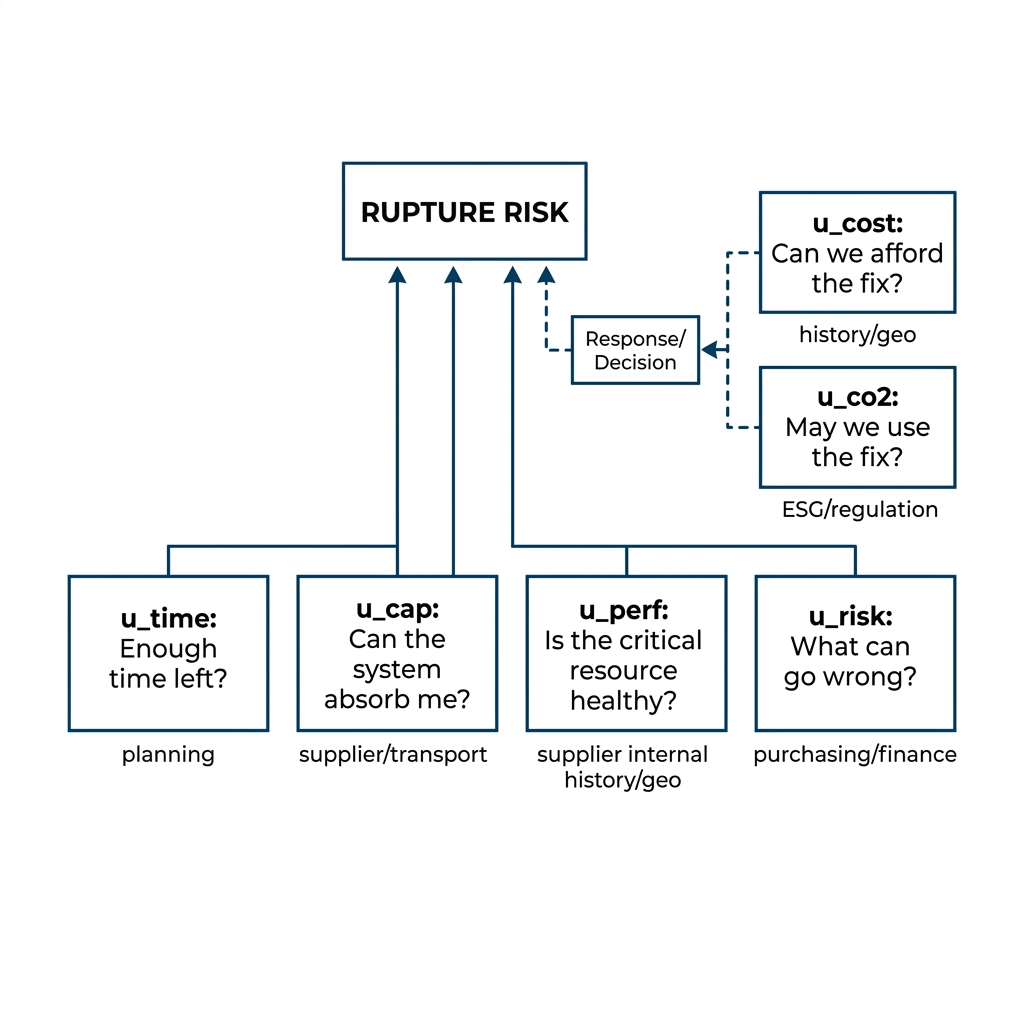
\includegraphics[width=0.85\linewidth]{Images/4.Operations/causal_tree_blocks.png}
    \caption{Causal structure behind the six-block selection: four direct rupture mechanisms and two arbitration variables.}
    \label{fig:todraw_blocks}
\end{figure}

\paragraph{Local Declared Urgency ($U_{d,\text{local}}$).}
Symmetrically to real urgency, declared urgency is not read as a single free-text estimate: it is reconstructed from a structured elicitation, so that it can be scored, propagated, and compared to $U_{r,\text{local}}$ on the same $[0,1]$ scale. At each node, the operator compares four criteria pairwise through the Analytic Hierarchy Process (\gls{ahp}), which yields a consistency-checked weight $w_j$ per criterion, then rates each criterion on a severity scale $s_j \in \{1, \ldots, 9\}$. Local declared urgency is the weight-averaged severity, rescaled to $[0,1]$:
\begin{equation}
    U_{d,\text{local}} = \sum_{j=1}^{4} w_j\,\frac{s_j - 1}{8}, \qquad \sum_{j=1}^{4} w_j = 1.
    \label{eq:ud_local}
\end{equation}
The elicitation tool itself, its four criteria, and the consistency gate that rejects an incoherent weight vector before it reaches this formula are application choices, described in Section~\ref{sec:ahp_tool}. What matters at this stage is that $U_{d,\text{local}}$ and $U_{r,\text{local}}$ (Equation~\ref{eq:ur_local}) are both bounded, node-local quantities in $[0,1]$ before either one is propagated, since the propagation equations below require both of them already defined.

\paragraph{Network Propagation.}
Declared urgency $U_d$ propagates \emph{downstream}, from the final customer (rank~0) toward raw-material suppliers, while real urgency $U_r$ propagates \emph{upstream}, from suppliers toward the final customer, using a leaky product rule that keeps both signals bounded in $[0,1]$ and monotonically increasing as more neighbours become urgent:
\begin{align}
    U_{d,i} &= 1 - \bigl(1 - U_{d,\text{local},i}\bigr) \prod_{k \in \text{Succ}(i)} \bigl(1 - \gamma_{ik} U_{d,k}\bigr), \label{eq:ud_prop} \\
    U_{r,i} &= 1 - \bigl(1 - U_{r,\text{local},i}\bigr) \prod_{j \in \text{Pred}(i)} \bigl(1 - \beta_{ji} U_{r,j}\bigr), \label{eq:ur_prop}
\end{align}
where $\gamma_{ik} \in [0,1]$ is the downstream attenuation coefficient on arc $(i,k)$ and $\beta_{ji} \in [0,1]$ is the upstream amplification coefficient on arc $(j,i)$. Backup arcs are purely documentary and inert with respect to both propagations. Table~\ref{tab:propagation_components} details the propagation variables.

\begin{table}[H]
\centering
\caption{Component definitions for the network propagation equations.}
\label{tab:propagation_components}
\small
\begin{tabularx}{\linewidth}{llX}
\toprule
\textbf{Component} & \textbf{Type} & \textbf{Description} \\
\midrule
$U_{d,i}$, $U_{r,i}$ & Dependent variables & Propagated declared/real urgency at node $i$ \\
$U_{d,\text{local},i}$, $U_{r,\text{local},i}$ & Input variables & Local urgency at node $i$ after status-rule adjustment \\
$\gamma_{ik}$ & System parameter & Downstream (demand) attenuation coefficient on arc $i \to k$ \\
$\beta_{ji}$ & System parameter & Upstream (risk) amplification coefficient on arc $j \to i$ \\
$\text{Succ}(i)$, $\text{Pred}(i)$ & Structural sets & Nominal (non-backup) successors and predecessors of node $i$ \\
\bottomrule
\end{tabularx}
\end{table}

Propagation is recomputed incrementally: only the nodes downstream or upstream of a change (a submitted questionnaire, a revised KPI, a structural edit) are recalculated, rather than the full graph, which keeps the digital twin responsive as the network grows. Computation and propagation are triggered per node, not on a single synchronised clock: whenever a node's local urgency changes, whether from a submitted weekly review or a manual KPI edit, the system recomputes that node's aggregation and propagates the change through its upstream or downstream cone only (Section~\ref{sec:architecture}). Because each node is reviewed on its own weekly cadence rather than all at once, propagation across the network is continuous and asynchronous in practice, not a single global weekly batch; Section~\ref{sec:weekly_cycle} describes the review cadence itself.

\begin{figure}[H]
    \centering
    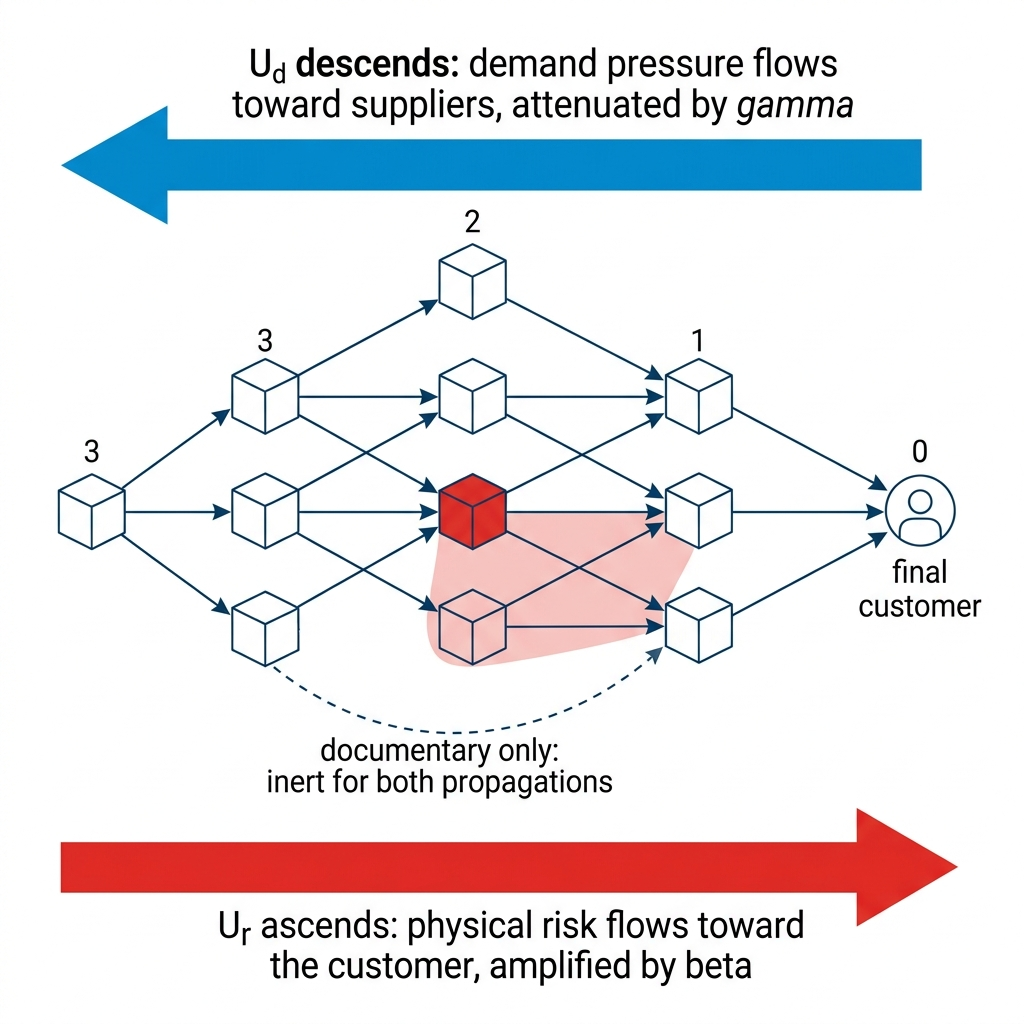
\includegraphics[width=0.85\linewidth]{Images/4.Operations/urgency_propagation.png}
    \caption{Bidirectional urgency propagation on the supply chain DAG.}
    \label{fig:todraw_propagation}
\end{figure}

\subsubsection{Core Model: Asymmetric Cognitive Adequacy (Prospect Theory)}

The mismatch between declared and real urgency is split into two named pathologies, false urgency $F$ (over-declaration, panic) and hidden risk $H$ (under-declaration, silent danger):
\begin{equation}
    F = \max(U_d - U_r,\, 0), \qquad H = \max(U_r - U_d,\, 0).
    \label{eq:fh}
\end{equation}
Drawing on Kahneman and Tversky's Prospect Theory~\autocite{kahneman1979prospect}, the two pathologies are penalised asymmetrically and with diminishing marginal sensitivity to large errors:
\begin{equation}
    \text{penalty} = \lambda_{\text{under}} H^{\alpha} + \lambda_{\text{over}} F^{\alpha},
    \label{eq:penalty}
\end{equation}
and the penalty is rescaled into an adequacy score $A \in [0, 100]$ through an exponential mapping bounded by the penalty of a maximal one-sided error:
\begin{equation}
    A = 100 \times \frac{\exp(-\text{penalty}) - \exp(-\text{penalty}_{\max})}{1 - \exp(-\text{penalty}_{\max})}, \qquad \text{penalty}_{\max} = \max(\lambda_{\text{under}}, \lambda_{\text{over}}).
    \label{eq:At}
\end{equation}
Table~\ref{tab:adequation_components} lists the parameters, with their governing constraint $\lambda_{\text{under}} > \lambda_{\text{over}}$: a coordinator who panics wastes premium transport capacity, but a coordinator who under-reports risk misses the window to prevent a line stoppage, so under-declaration is priced more expensively.

\begin{table}[H]
\centering
\caption{Component and parameter definitions for the asymmetric adequacy equations.}
\label{tab:adequation_components}
\small
\begin{tabularx}{\linewidth}{llXl}
\toprule
\textbf{Component} & \textbf{Type} & \textbf{Description} & \textbf{Default} \\
\midrule
$F$ & Dependent variable & False urgency (over-declaration) & n/a \\
$H$ & Dependent variable & Hidden risk (under-declaration) & n/a \\
$\lambda_{\text{under}}$ & System parameter & Penalty weight on hidden risk & $2.25$ \\
$\lambda_{\text{over}}$ & System parameter & Penalty weight on false urgency & $1.0$ \\
$\alpha$ & System parameter & Psychophysical curvature (diminishing sensitivity) & $0.88$ \\
$A$ & Dependent variable & Adequacy score, $100$ = perfect alignment & $[0,100]$ \\
\bottomrule
\end{tabularx}
\end{table}

The default $\lambda_{\text{under}}/\lambda_{\text{over}} = 2.25$ ratio reprises the loss-aversion coefficient measured by Kahneman and Tversky~\autocite{kahneman1979prospect,kahneman2011thinking}, and $\alpha = 0.88$ reprises their measured curvature of the value function. These defaults carry the status of literature-derived starting points, not measured properties of supply chain coordinators: they have not yet been validated empirically in this context, and their recalibration is one purpose of the validation campaign of Section~\ref{sec:serious_game}. Both the aggregation weights $\omega_m$ and the penalty parameters $(\lambda_{\text{under}}, \lambda_{\text{over}}, \alpha)$ are configurable per project rather than hard-coded, so that this recalibration requires no code change.

\subsubsection{Monte Carlo Estimate of the Time Block}
\label{sec:mc_criticality}

The analytic $u_{\text{time}}$ block assumes a Normal lead time at a single node. On a multi-tier network this assumption breaks: a node can only start when \emph{all} its predecessors have delivered, and the maximum of several skewed lead times has no convenient closed form. The module \texttt{mc/lead\_time.py} therefore replaces the analytic estimate with a stochastic one when enabled.

The simulation works in three steps. First, each node draws its lead time $L_i$ from a configurable distribution (lognormal, normal clipped to zero, or triangular). Second, completion times propagate along the DAG in topological order: a node starts when its last predecessor finishes ($S_i = \max_{j\in\text{Pred}(i)} C_j$) and completes after its own lead time ($C_i = S_i + L_i$). Third, the delay probability of each node is estimated as the fraction of draws in which it misses its deadline, $u_{\text{time}} = P(C_i > d_i)$, over $N=10\,000$ draws by default. A memory guardrail caps the simulation at $N \times n \le 5\times 10^7$ across $n$ nodes.

The estimate feeds directly into Equation~\ref{eq:ur_local} through a dedicated override point, so the aggregation, status rules, and propagation machinery are reused unchanged.

\subsubsection{Network Criticality Index}
\label{sec:criticality}

The criticality service (\texttt{services/criticite.py}) answers one question systematically: which node, if it failed completely, would cause the most damage to final-customer delivery? For every active node in turn, the service forces the node's local real urgency to $1.0$, re-runs the ascending propagation, and measures two deltas: the rise of $U_r$ at the final-customer nodes ($\Delta U_{r,\text{final}}$) and the largest rise anywhere in the network ($\Delta U_{r,\max}$). Every shock is run twice, once on the standard pipeline and once on an $\varepsilon$-regularised twin that carries the same computation in log-survival, $\ell(p) = -\ln(1-p)$, with urgency values clipped to $1-\varepsilon$ so that a survival product is never exactly zero. Nodes are ranked by $\Delta U_{r,\text{final}}$ first, then by $\Delta \ell_{\text{final}}$, then by name. The reason for that second key is the saturation behaviour described below.

A small example makes the mechanics concrete. Take a three-node chain, raw-material supplier $\to$ sub-assembly $\to$ final assembly, with upstream coefficients $\beta = 0.9$ then $0.7$, and a baseline where the sub-assembly node carries $U_{r} = 0.40$ and the final node $U_r = 0.28$. Forcing the sub-assembly node to $U_r = 1.0$ propagates to the final node as $1-(1-0.7\times1.0) = 0.70$, so its shock deltas are $\Delta U_{r,\text{final}} = 0.70-0.28 = 0.42$ and $\Delta U_{r,\max} = 1.0-0.40 = 0.60$ (Figure~\ref{fig:criticite}).

One behaviour of this index matters for interpretation: a node already saturated at $U_r \ge 1.0$ yields a delta of zero and sinks to the bottom of the ranking, since its risk is already realised in the baseline. In a network-wide crisis, where many nodes saturate at once, $\Delta U_r$ collapses to zero everywhere and the ranking degenerates, which is precisely the situation in which it would be most useful: nine of the nineteen turns of the campaign of Section~\ref{sec:serious_game} were saturated, and the exclusion rule used by hypothesis H3 was written for that reason.

The $\Delta \ell$ key is the answer to it. Because $\ell(p) = -\ln(1-p)$ is strictly increasing, $\Delta \ell_{\text{final}}$ and $\Delta U_{r,\text{final}}$ are two monotone transforms of the same shocked urgency at the final customer, so outside saturation they induce the same order and the ranking is unchanged; this is stated as a property-based invariant and tested as one. Inside saturation the clip that flattens $\Delta U_r$ does not flatten $\Delta \ell$, which keeps measuring how much deeper the shock drives an already saturated network, so the nodes that $\Delta U_r = 0$ made indistinguishable are separated again. Measured on the campaign turns, the number of turns on which the deep suppliers can be ordered at all rises from 10 to 17 out of 19.

\begin{figure}[H]
    \centering
    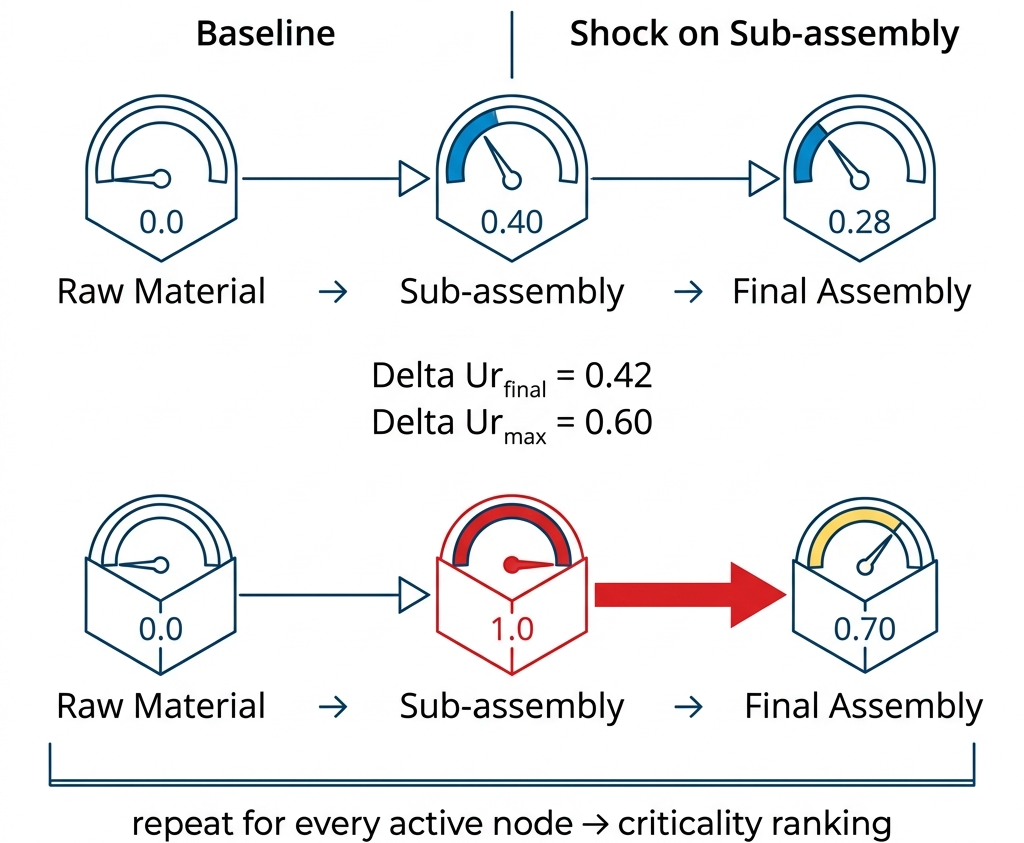
\includegraphics[width=0.85\linewidth]{Images/4.Operations/shock_simulation.png}
    \caption{One iteration of the systematic shock simulation behind the criticality index.}
    \label{fig:todraw_shock}
\end{figure}

\paragraph{Probabilistic Criticality.}
The sweep above answers what happens if a node fails \emph{completely}, which is a worst case rather than an expectation. A second entry point answers the distributional question on the same machinery. Instead of forcing $U_{r,\text{local}} = 1.0$, it draws shock severities from the graduated flat-rate severities of the calibrated event engine: minor, major and critical failures at $0.4$, $0.7$ and $1.0$, and financial alerts at $0.3$, $0.6$ and $0.9$, the two families weighted equally and, within a family, weighted by decreasing field frequency ($0.6$, $0.3$, $0.1$), since benign incidents are markedly more common than outright defaults. Each draw is applied as a ratchet, $\max(U_{r,\text{local}}, \text{severity})$, on the same principle as the event engine: a failure never improves a node's state. The whole batch is then propagated in one vectorised pass, in duplicate for $\Delta U_r$ and $\Delta \ell$. Each node receives $P(\Delta U_{r,\text{final}} > 0.2)$ and the median and ninth-decile of its $\Delta \ell_{\text{final}}$ distribution. The computation is read-only, seeded and deterministic, so the same inputs give the same ranking.

\begin{figure}[H]
    \centering
    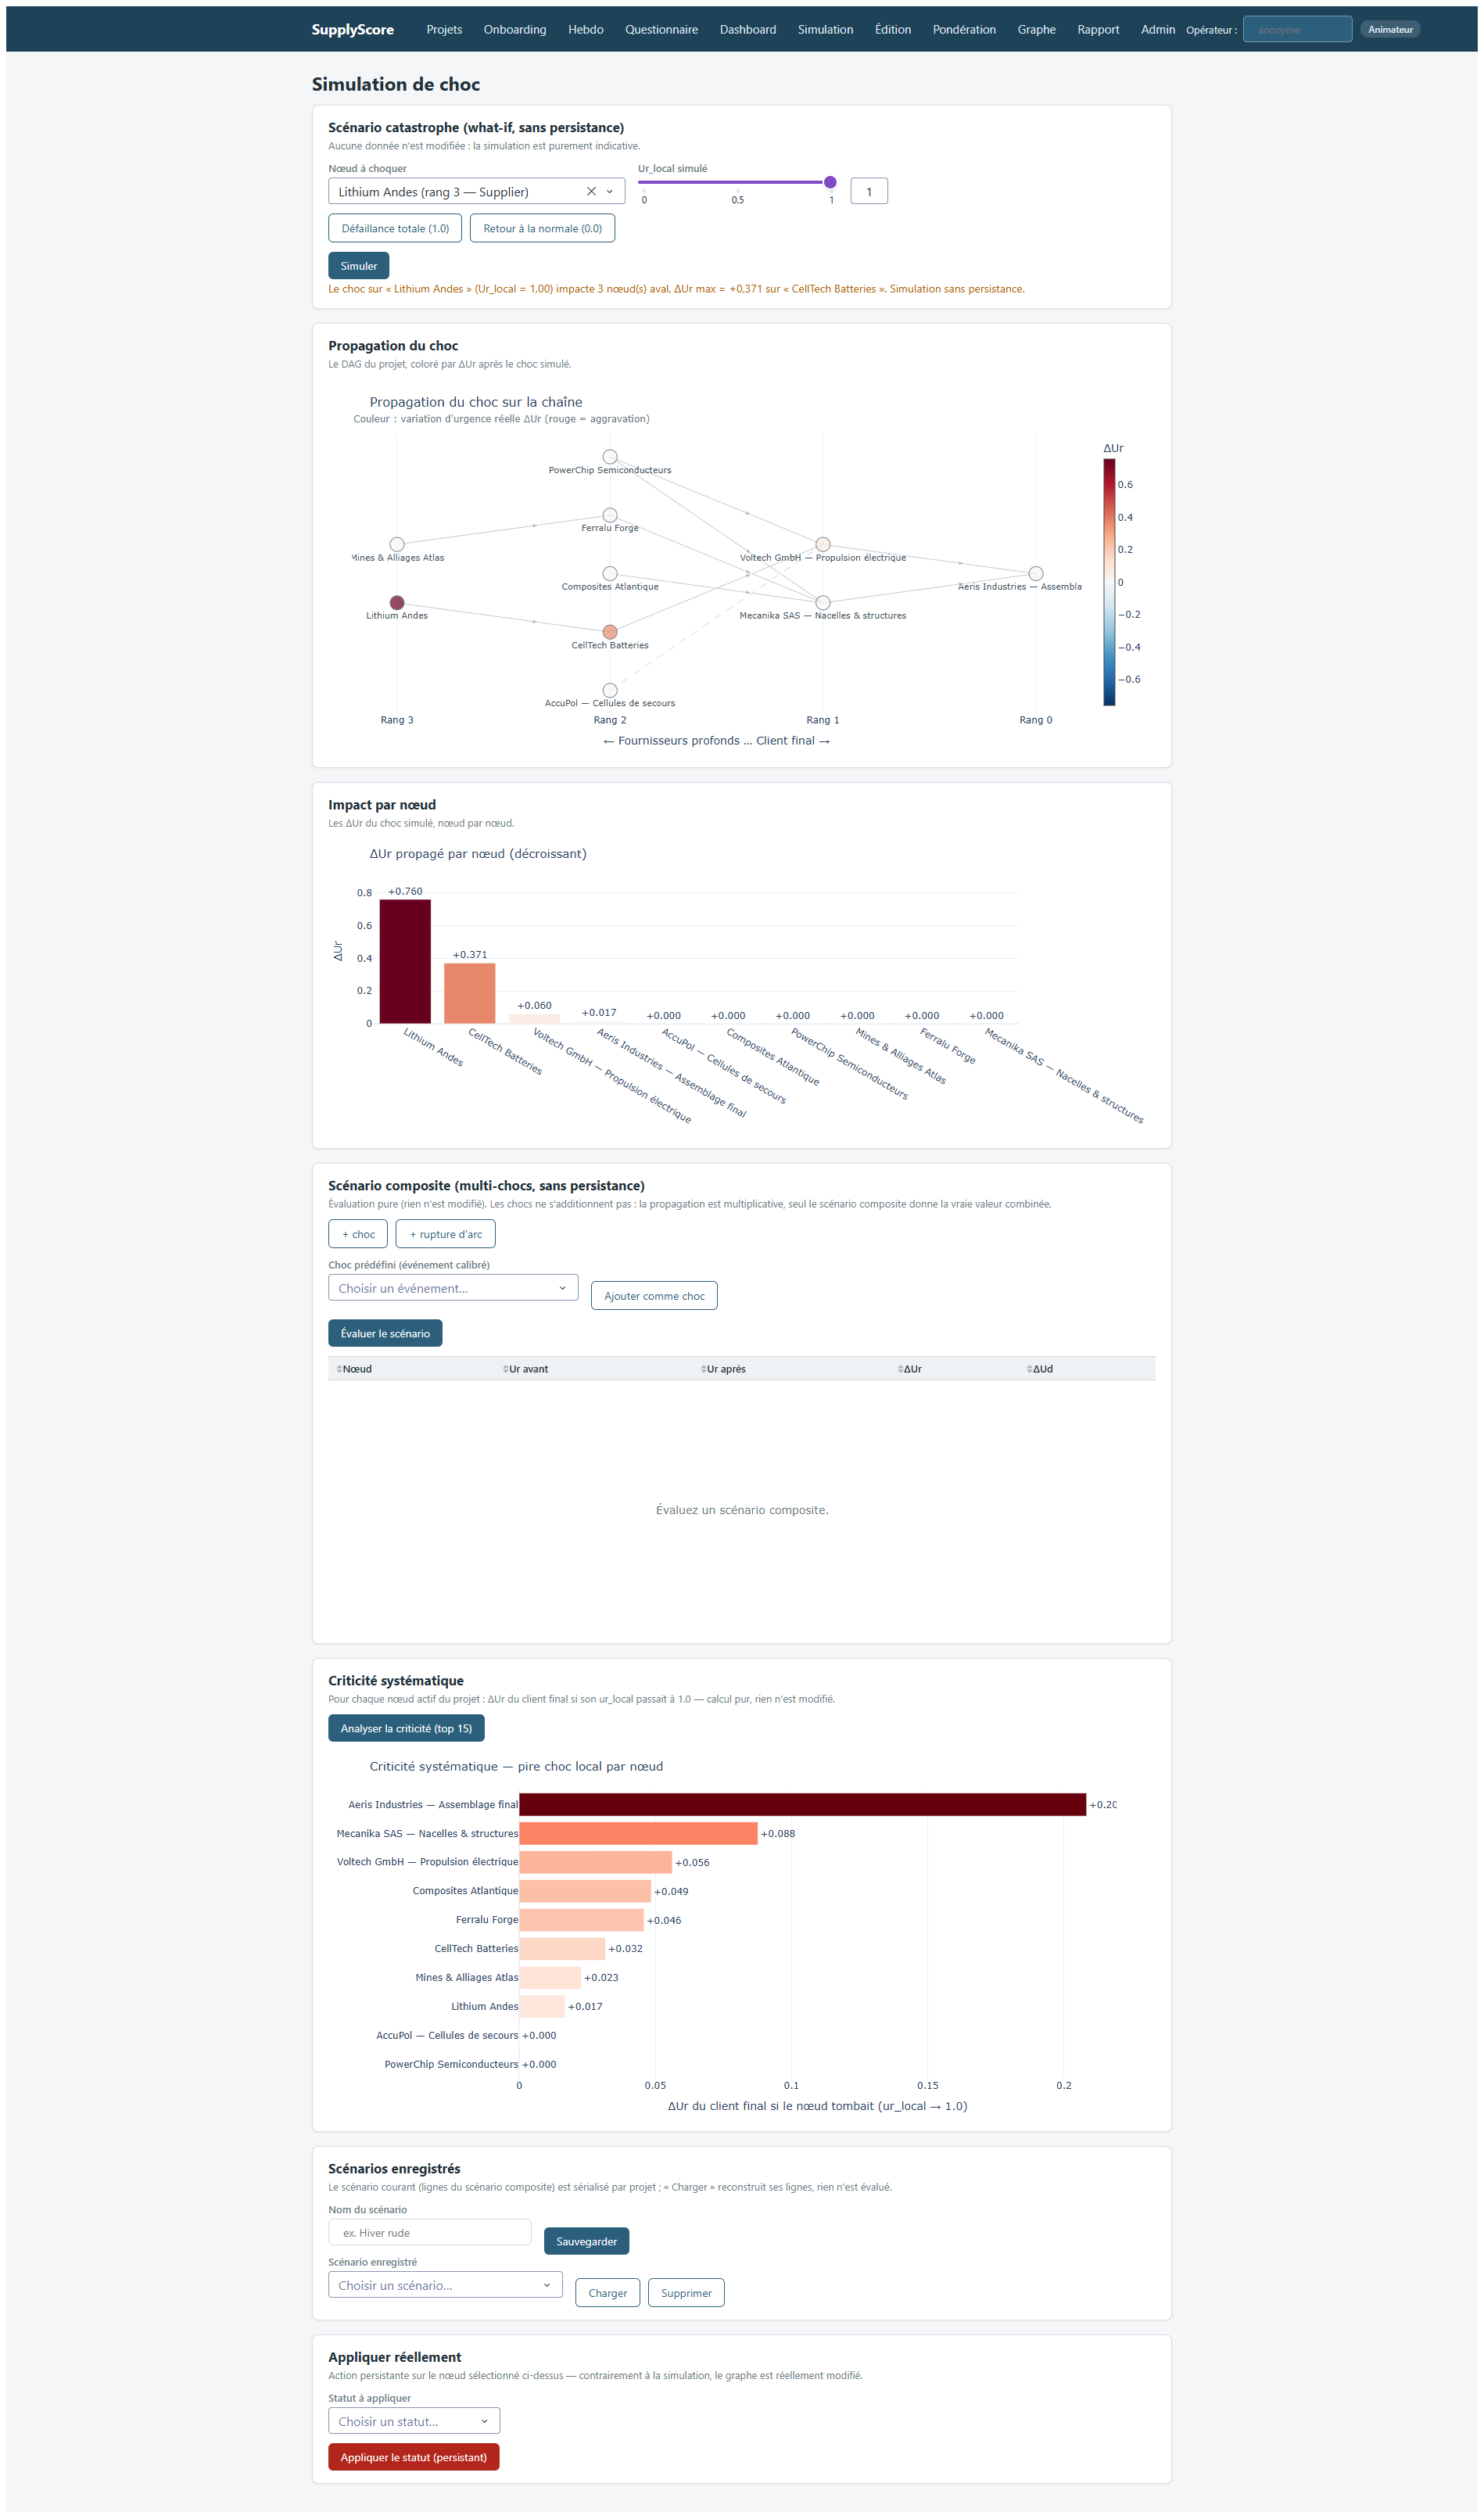
\includegraphics[width=0.85\linewidth]{Images/4.Operations/criticite.png}
    \caption{Network criticality ranking after a systematic shock simulation.}
    \label{fig:criticite}
\end{figure}

%% ═══════════════════════════════════════════════════════════════════════════
\subsection{Application and Implementation Choices}
\label{sec:application}
%% ═══════════════════════════════════════════════════════════════════════════

The model above is deliberately silent on tooling. This section describes how each mathematical object it defines is actually elicited from an operator, computed inside the running system, exposed back to a coordinator, and kept safe: the system architecture, the AHP and Fuzzy-BWM/PROMETHEE elicitation tools, the weekly operating cycle and event engine that keep KPI data current, and the explainability, export, and hardening capabilities built on top.

\subsubsection{System Architecture}
\label{sec:architecture}

Several design guarantees relied upon elsewhere in this document, auditability, multi-tenant isolation, deterministic testing, are architectural choices, not mathematical ones, and are described here on their own.

\paragraph{Single facade.} All operations go through one orchestrating facade
(\texttt{services/}\allowbreak\texttt{orchestrator.py}), which coordinates the mathematical core, the
graph repository, and the persistence layers behind a single thread-safe entry
point. The web interface, the command-line entry point, and the test suite all
drive the system exclusively through this facade; there is no second write path.

\paragraph{Multi-tenant persistence.} Data is split between one global registry
database (projects, nodes, arcs, milestones, scenarios, registry-level audit) and
one SQLite database per node holding its private operational history (KPI
snapshots, AHP assessments, weekly reviews, urgency history, declared events, and
a per-node audit log). This isolation prevents write contention between operators
reviewing different nodes and enforces the boundary that one supplier's raw
history is not readable through another supplier's records.

\paragraph{Gatekeeper writes.} Every business write crosses a single mutation
service that whitelists the touched fields, validates ranges, diffs against the
current state (a no-op write leaves no trace), records the change in the audit
log with its author and source, and synchronises the in-memory graph. Audit
tables are strictly immutable, including from the administration interface:
the "no silent data loss" guarantee is enforced here, not by convention.

\paragraph{Graph and propagation.} The network lives in an in-memory graph
repository (networkx-backed; a Neo4j adapter is scaffolded but out of scope).
Propagation is incremental: only the upstream/downstream cones of nodes whose
local urgency actually changed are recomputed, which keeps the twin responsive
at the 1000+-node scale validated by dedicated performance benchmarks.

\begin{figure}[H]
    \centering
    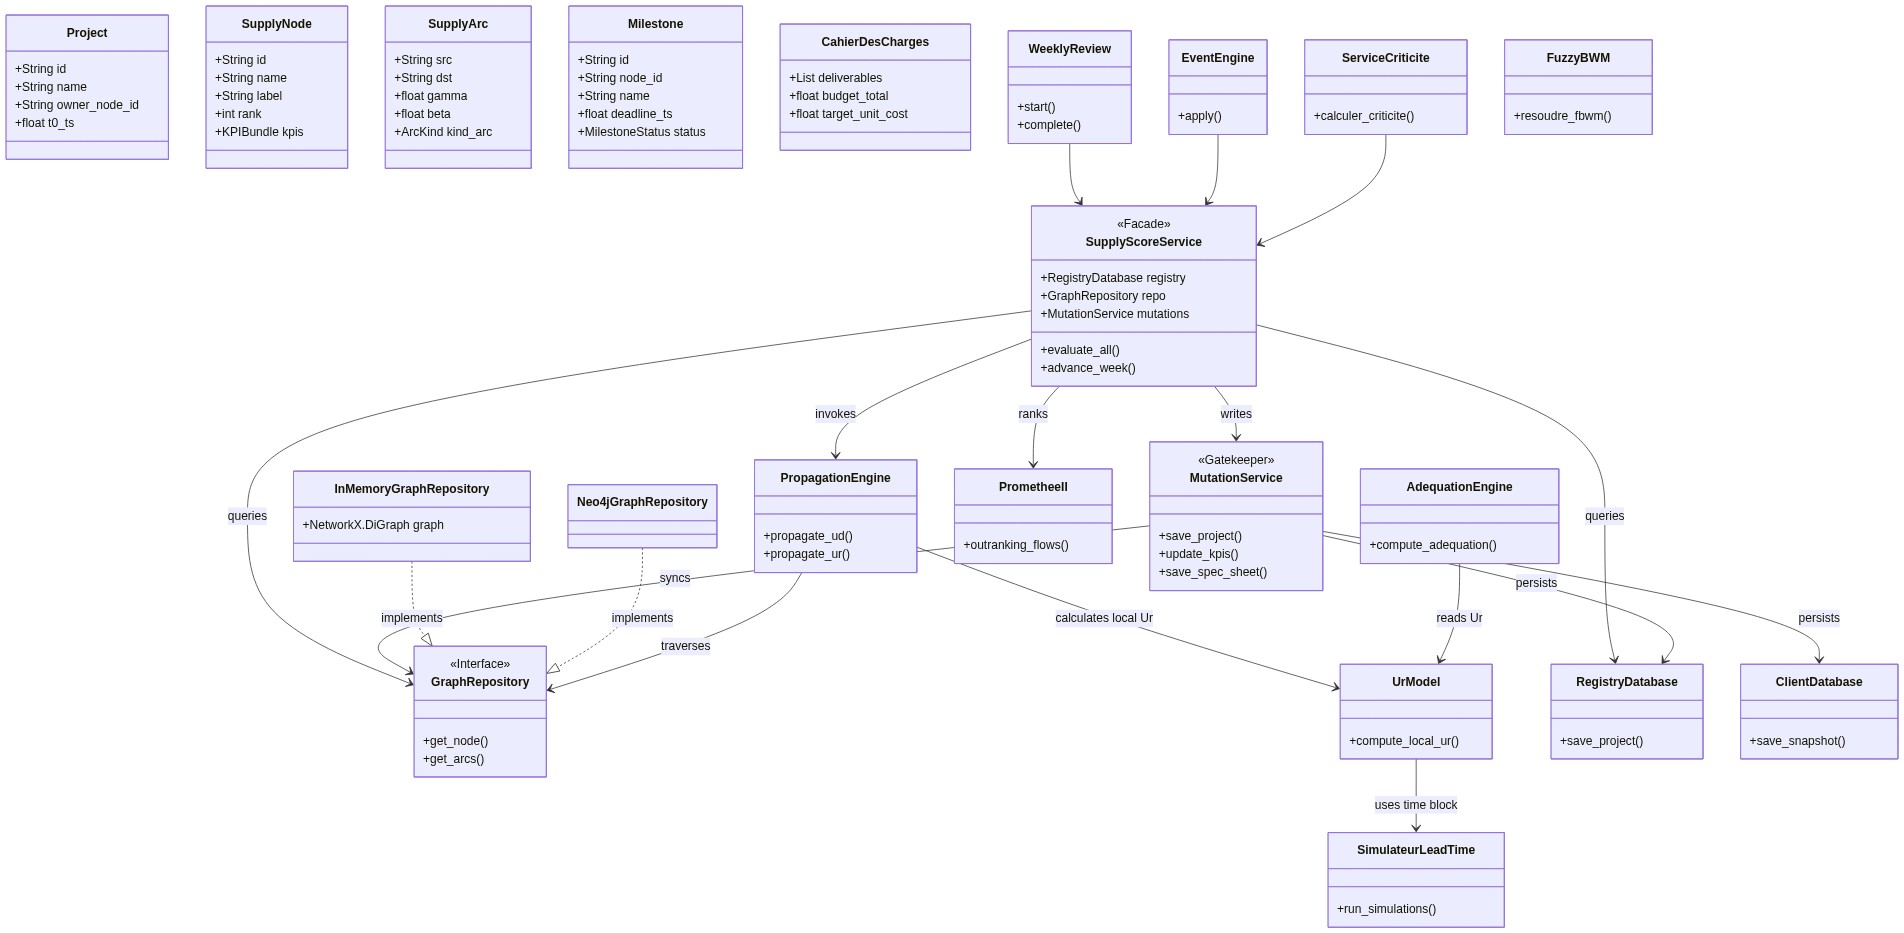
\includegraphics[width=0.85\linewidth]{Images/4.Operations/uml_architecture.png}
    \caption{Doxygen-generated UML view of the SupplyScore architecture: single facade, gated writes, multi-tenant persistence.}
    \label{fig:todraw_architecture}
\end{figure}

\paragraph{Decoupled clocks.} Each project carries its own clock: a system clock
for live use, a game clock advancing week by week for serious-game sessions, and
a fixed clock for deterministic tests. The weekly cycle, milestone pressure, and
event timestamps all read the project clock, never the wall clock directly,
which is what makes a compressed serious-game campaign (Section~\ref{sec:serious_game})
possible without touching the model.

\subsubsection{Expert Criteria Weighting: The AHP Elicitation Model}
\label{sec:ahp_tool}

The Python module \texttt{core/ahp.py} implements the Saaty
eigenvector method for a 4-criterion questionnaire administered through the weekly
review page, and is the tool that produces $U_{d,\text{local}}$ (Equation~\ref{eq:ud_local}). The four criteria are:

\begin{enumerate}[label=\textbf{C\arabic*.}]
    \item \textit{Operational impact}: ``If this task fails, what is the downstream
          consequence?''
    \item \textit{Time window}: ``How long before the situation becomes irredeemable?''
    \item \textit{Downstream dependencies}: ``How many tasks are blocked waiting for
          this one?''
    \item \textit{Recoverability}: ``Can we catch up if this task is late?''
          (inverted, where lower is worse)
\end{enumerate}

\paragraph{How the Four Criteria Were Chosen.}
The criteria set follows from two constraints, one cognitive and one structural. Cognitively, Saaty's method degrades as the number of pairwise-compared criteria grows: consistency becomes hard to maintain beyond roughly seven items, and each additional criterion adds $n-1$ comparisons to the operator's weekly workload~\autocite{saaty1990how,triantaphyllou2024}. Keeping $n=4$ limits the questionnaire to six comparisons, short enough for a weekly cadence. Structurally, the four questions mirror the way declared urgency is consumed downstream: C1 (impact) and C3 (dependencies) capture the \emph{severity} dimension that propagation amplifies across the network, C2 (time window) captures the \emph{slack} dimension confronted with the $u_{\text{time}}$ block of Section~\ref{sec:math_framework}, and C4 (recoverability) captures the \emph{resilience} dimension confronted with the recovery term of $u_{\text{risk}}$. Each declared criterion therefore has an operational counterpart in the computed signal, which is what makes the later $U_d$ vs.\ $U_r$ comparison meaningful rather than a comparison of unrelated quantities. Larger criteria sets (cost, sustainability) are deliberately routed to the F-BWM weighting of the KPI blocks instead (Section~\ref{sec:fbwm_promethee}), where the elicitation burden is lower.

\begin{figure}[H]
    \centering
    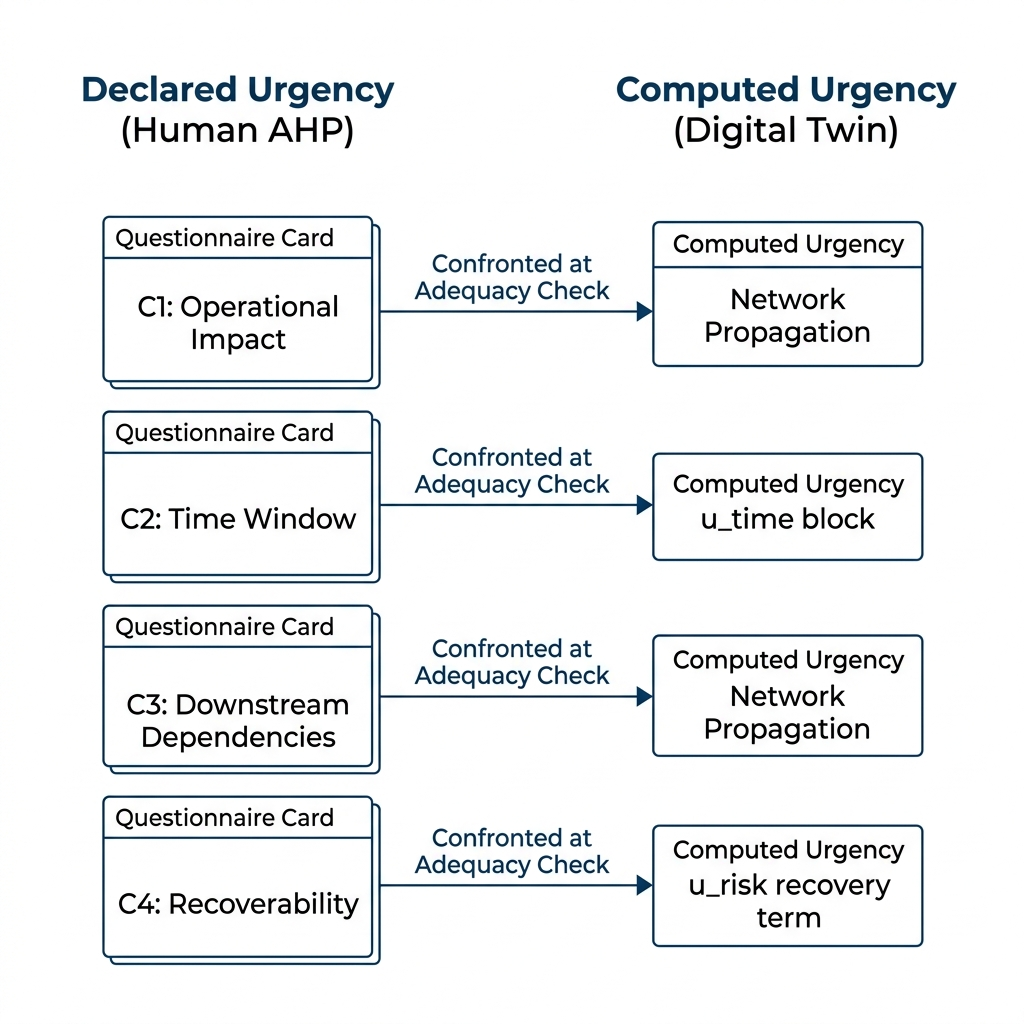
\includegraphics[width=0.85\linewidth]{Images/4.Operations/ahp_criteria_mapping.png}
    \caption{Correspondence between the four AHP criteria and their computed counterparts.}
    \label{fig:todraw_criteria}
\end{figure}

The consistency ratio is computed as:
\begin{equation}
    \gls{cr} = \frac{\gls{ci}}{\gls{ri}[n]},
    \label{eq:ahp_cr}
\end{equation}
where the components of the consistency assessment are defined in Table~\ref{tab:ahp_cr_components}.

\begin{table}[H]
\centering
\caption{Component definitions for the AHP consistency ratio equation.}
\label{tab:ahp_cr_components}
\small
\begin{tabularx}{\linewidth}{llX}
\toprule
\textbf{Component} & \textbf{Type} & \textbf{Description} \\
\midrule
$\gls{cr}$ & Dependent variable & Consistency Ratio of the pairwise comparison matrix \\
$\gls{ci}$ & Dynamic variable   & Consistency Index computed from the matrix principal eigenvalue \\
$\gls{ri}[n]$ & System parameter & Random Index for a matrix of size $n$ (from Saaty's reference table) \\
\bottomrule
\end{tabularx}
\end{table}

using Saaty's Random Index table. If $\gls{cr} > 0.10$, the interface flags the questionnaire as inconsistent and invites the operator to revise the most contradictory pairwise comparison before the assessment is accepted. Declared urgency is further smoothed with an exponential moving average ($\rho = 0.3$) across consecutive weekly assessments, absorbing transient stress spikes without erasing a sustained change in perception.

\begin{figure}[H]
    \centering
    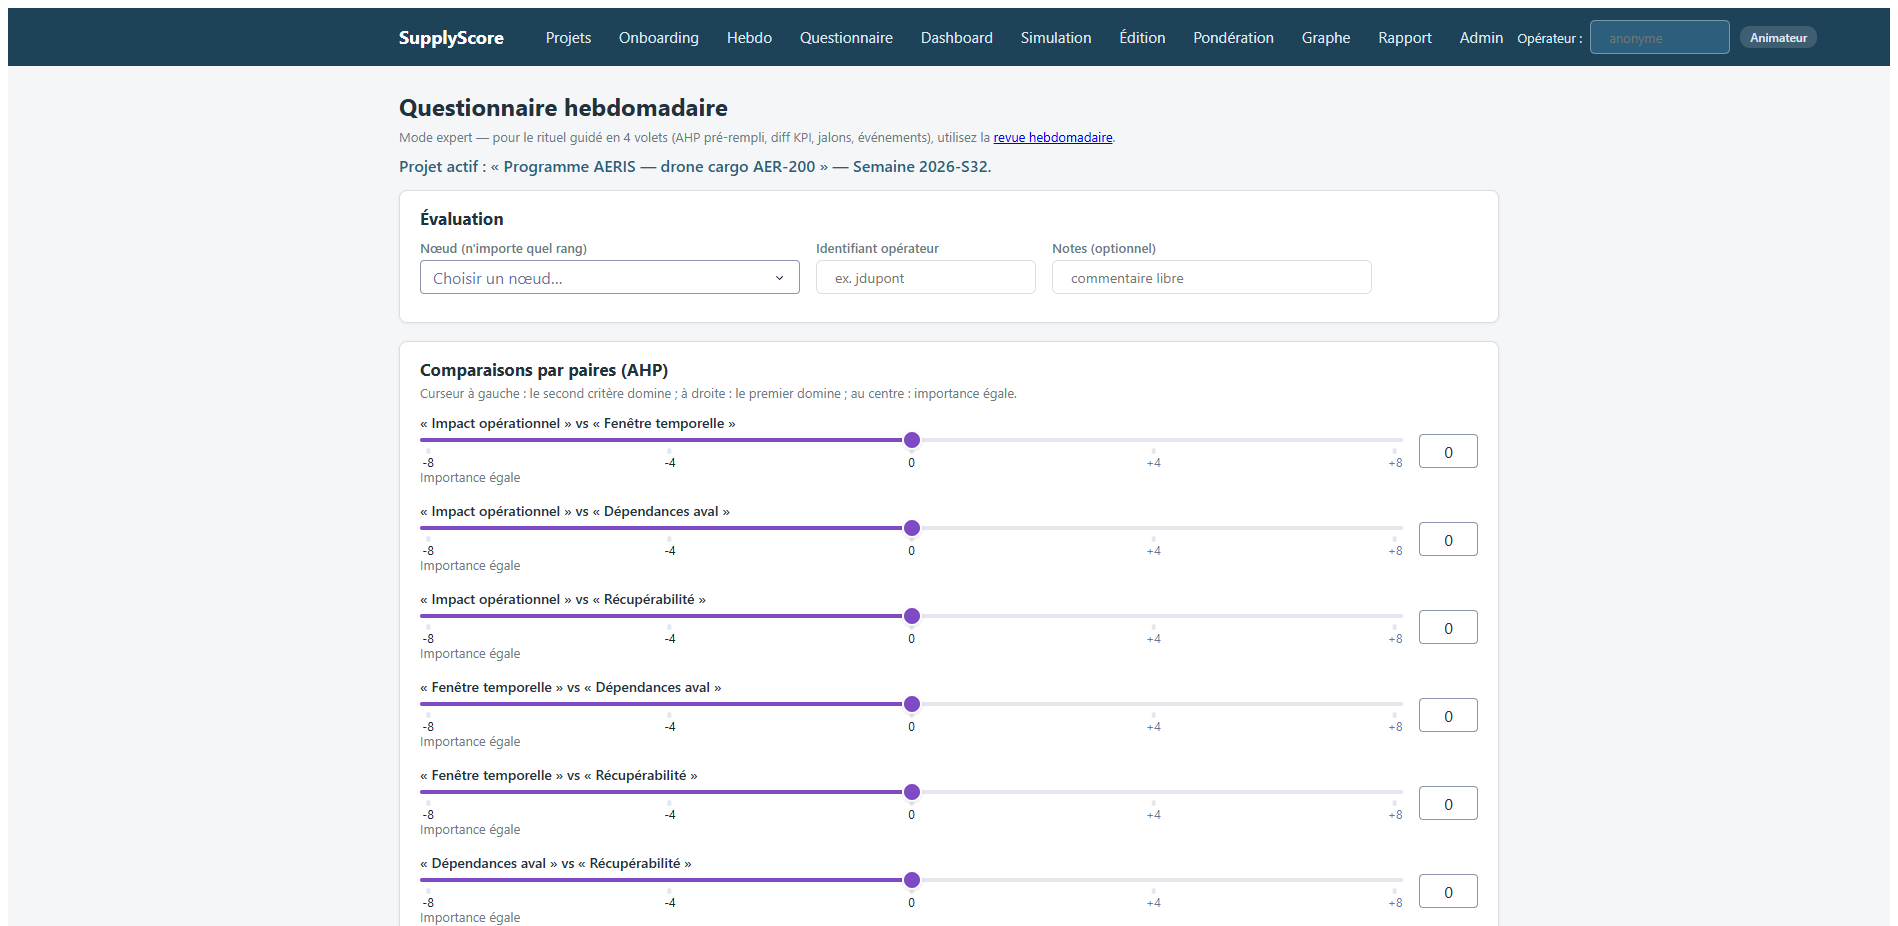
\includegraphics[width=0.85\linewidth]{Images/4.Operations/questionnaire_screenshot.png}
    \caption{AHP questionnaire page with the consistency-ratio validation gate.}
    \label{fig:todraw_questionnaire}
\end{figure}

AHP is viable for $U_d$ encoding in this context. The
$\gls{cr}$ validation gate, exercised by both worked examples and automated tests, detects and rejects cognitively inconsistent
expert inputs before they enter the network. Its behaviour with real operators is measured in the campaign of Section~\ref{sec:serious_game}.

%% ═══════════════════════════════════════════════════════════════════════════
\subsubsection{Stochastic Judgment Modeling: Fuzzy BWM and PROMETHEE II Network Outranking}
\label{sec:fbwm_promethee}
%% ═══════════════════════════════════════════════════════════════════════════

The modules \texttt{mcda/fbwm.py} and \texttt{mcda/promethee.py} implement
two complementary methods: F-BWM offers a lower-effort elicitation route than crisp AHP for
weighting the six KPI blocks, and PROMETHEE~II turns those weights into a network-wide,
non-compensatory ranking of nodes that complements the per-node adequacy score.

\paragraph{F-BWM Implementation.}
The linguistic TFN scale maps five qualitative judgements to triangular fuzzy numbers on a
1--4.5 scale (from \textit{equally important} to \textit{absolutely more important}), each carrying
its own maximum consistency index. The consistency ratio of the Fuzzy BWM model is formulated as:
\begin{equation}
    \gls{cr}_{\text{BWM}} = \frac{\xi^*}{\text{CI}},
    \label{eq:bwm_cr}
\end{equation}
where $\xi^*$ is the optimal consistency indicator returned by a constrained non-linear
optimisation that fits the fuzzy weights to the elicited Best-to-Others and
Others-to-Worst comparisons, and $\text{CI}$ is read from the strongest linguistic judgement used.
If the optimisation fails to converge, the implementation falls back to uniform weights rather than
raising an error, so that a single malformed elicitation cannot crash the weekly review. Fuzzy
weights are defuzzified with the Graded Mean Integration Representation (GMIR):
\begin{equation}
    w_j = \frac{a_j + 4 b_j + c_j}{6},
    \label{eq:bwm_defuzz}
\end{equation}
then renormalised so that $\sum_j w_j = 1$. Table~\ref{tab:bwm_defuzz_components} defines the terms; the triangular fuzzy bounds are written $(a_j, b_j, c_j)$ here, rather than the more common $(l_j, m_j, u_j)$ notation, to avoid colliding with the risk blocks $u_m$ used throughout Section~\ref{sec:math_framework}.

\begin{table}[H]
\centering
\caption{Component definitions for the Fuzzy BWM defuzzification.}
\label{tab:bwm_defuzz_components}
\small
\begin{tabularx}{\linewidth}{llX}
\toprule
\textbf{Component} & \textbf{Type} & \textbf{Description} \\
\midrule
$w_j$ & Dependent variable & Crisp normalized weight of criterion $j$ \\
$a_j, b_j, c_j$ & Dynamic variables & Lower, modal, and upper bounds of the triangular fuzzy weight \\
$\xi^*$ & Dynamic variable & Optimal consistency indicator from the fitted optimisation \\
\bottomrule
\end{tabularx}
\end{table}

\paragraph{PROMETHEE~II Implementation.}
PROMETHEE~II is applied in production to rank the active nodes of a project on the same six
weighted urgency blocks (Table~\ref{tab:ur_blocks}) that feed local real urgency, giving
coordinators a network-wide, non-compensatory view of which nodes are collectively driving
urgency. For each pair of active nodes $(a,b)$ and each block $m$, the preference intensity
$P_m(g_m(a) - g_m(b)) \in [0,1]$ is computed with a Type~V linear preference function with an
indifference threshold; the aggregated preference index and net outranking flow follow the
standard PROMETHEE~II formulation:
\begin{equation}
    \pi(a,b) = \sum_m \omega_m P_m\bigl(g_m(a) - g_m(b)\bigr), \qquad \phi(a) = \phi^+(a) - \phi^-(a),
    \label{eq:promethee_net}
\end{equation}
where $\phi^+(a)$ and $\phi^-(a)$ are the average preference of $a$ over, respectively by, all
other active nodes. Table~\ref{tab:promethee_net_components} defines the outranking flow terms.

\begin{table}[H]
\centering
\caption{Component definitions for the PROMETHEE II net flow.}
\label{tab:promethee_net_components}
\small
\begin{tabularx}{\linewidth}{llX}
\toprule
\textbf{Component} & \textbf{Type} & \textbf{Description} \\
\midrule
$\pi(a,b)$ & Dependent variable & Aggregated preference index of $a$ over $b$ \\
$\phi(a)$ & Dependent variable & Net outranking flow representing overall preference ($\in [-1, 1]$) \\
$\phi^+(a)$, $\phi^-(a)$ & Dynamic variables & Positive (dominance) and negative (dominated) outranking flows \\
\bottomrule
\end{tabularx}
\end{table}

The same weights $\omega_m$ used in the local urgency aggregation (Equation~\ref{eq:ur_local}) are
reused as the PROMETHEE criteria weights, so that the network ranking and the per-node urgency
score remain mutually consistent rather than relying on a separately calibrated weight set.
Both modules are unit tested and wired into the production ranking path
(\texttt{services/}\allowbreak\texttt{orchestrator.py}).

%% ═══════════════════════════════════════════════════════════════════════════
\subsubsection{Weekly Review Cycle and Calibrated Event Engine}
\label{sec:weekly_cycle}
%% ═══════════════════════════════════════════════════════════════════════════

The weekly review cycle is what keeps the digital twin's KPI state current without free-form manual data entry: every write is structured, signed, and auditable. This section describes the cycle itself, then the calibrated event engine that translates real-world disruptions into KPI updates.

\paragraph{The Weekly Cycle.} The system is operated as a serious game advancing in discrete weeks (\texttt{core/clock.py} implements \texttt{SystemClock} for live use, \texttt{GameClock} for week-by-week advancement, and \texttt{FixedClock} for deterministic testing). At each new week, every active node is flagged as due for review, and the operator completes four sequential sections (\texttt{services/weekly.py}, served by the \texttt{/hebdo} page, Figure~\ref{fig:hebdo}):
\begin{enumerate}
    \item the AHP questionnaire, pre-filled with the previous week's values, with a one-click "unchanged" confirmation;
    \item the week's KPI values, shown against the previous week for quick differencing;
    \item progress on active milestones, compared against theoretical planning progress;
    \item any supply chain events that occurred during the week.
\end{enumerate}
All four sections are written as a single signed, atomic transaction, so that no partial or anonymous review can corrupt the node's history.

\begin{figure}[H]
    \centering
    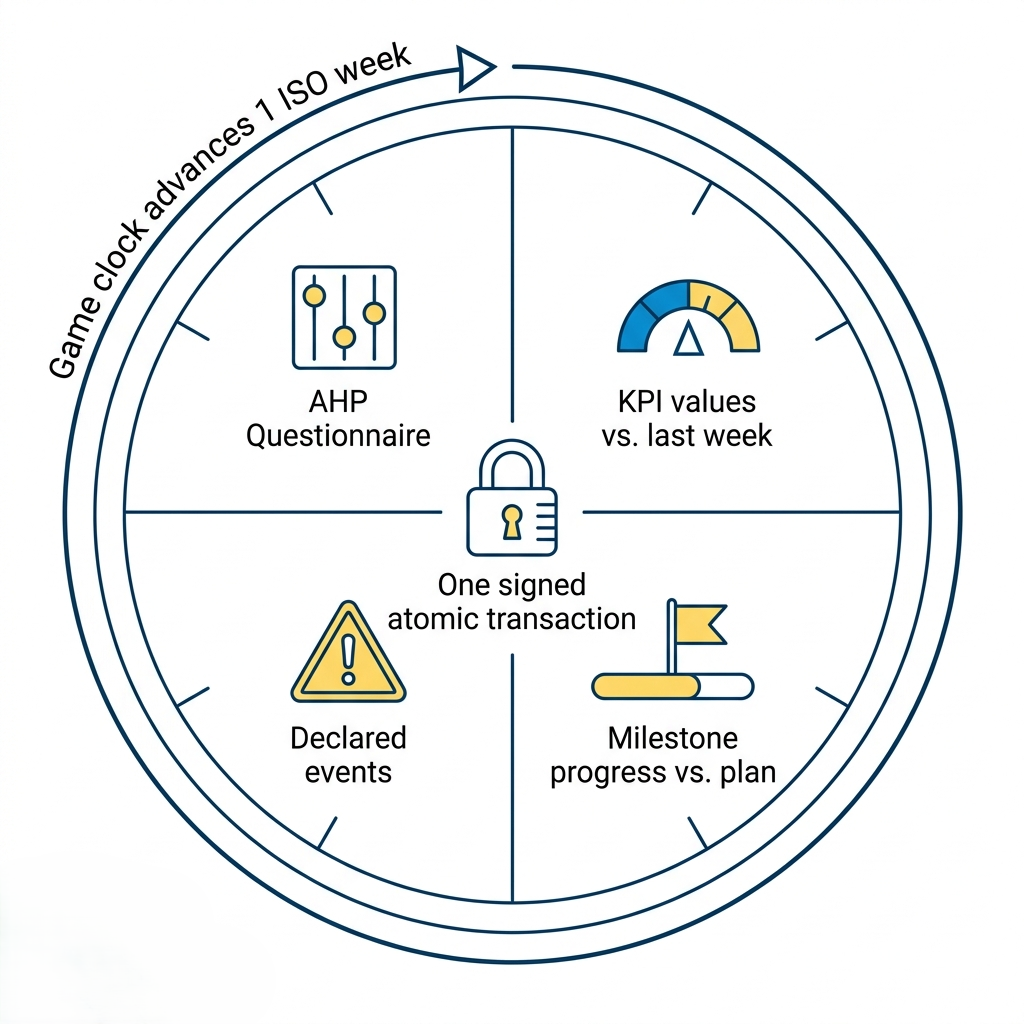
\includegraphics[width=0.85\linewidth]{Images/4.Operations/weekly_cycle.png}
    \caption{The four-section weekly review cycle committed as a single signed transaction.}
    \label{fig:todraw_weekly}
\end{figure}

\begin{figure}[H]
    \centering
    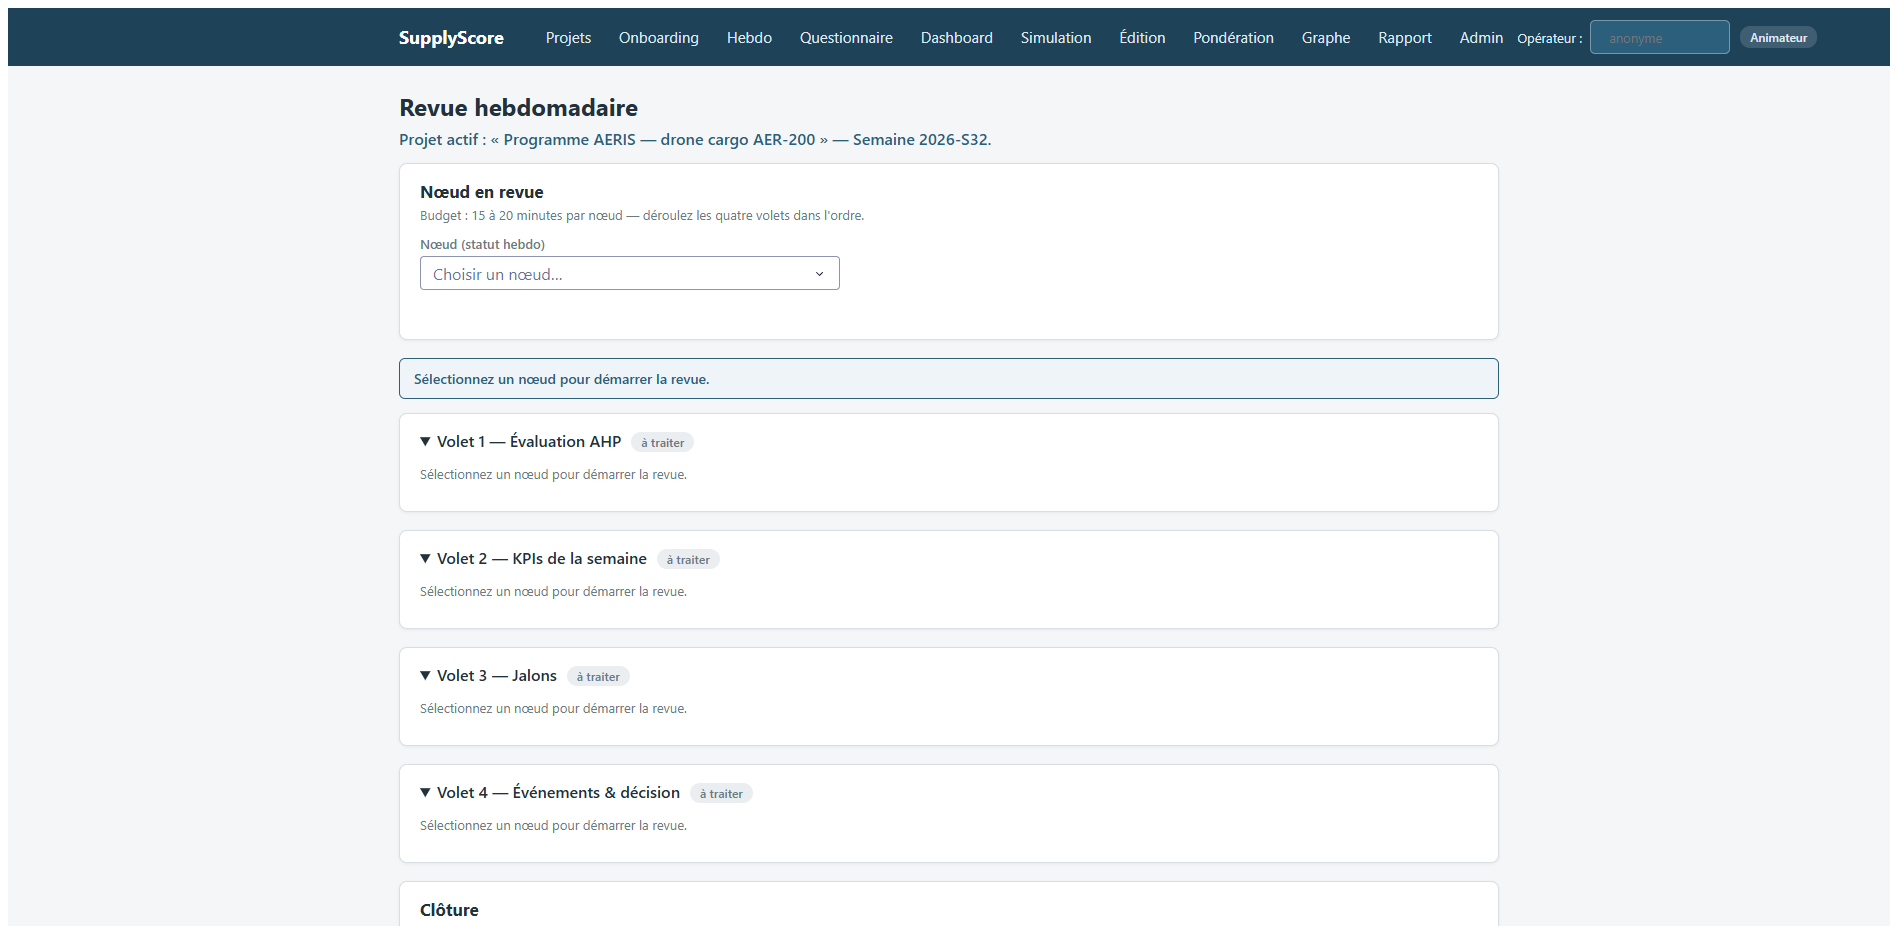
\includegraphics[width=0.85\linewidth]{Images/4.Operations/hebdo.png}
    \caption{Weekly review page: the four sequential sections (AHP, KPIs, milestones, events).}
    \label{fig:hebdo}
\end{figure}

\paragraph{Calibrated Event Engine.}
Rather than asking operators to manually recompute the KPI impact of a disruption, the system exposes a taxonomy of fourteen calibrated event types (\texttt{domain/events.py}), listed in Table~\ref{tab:event_types}, each mapped to one or more KPI updates through one of three calibration operators.

\begin{table}[H]
\centering
\caption{The fourteen calibrated event types.}
\label{tab:event_types}
\small
\begin{tabularx}{\linewidth}{XXX}
\toprule
\texttt{panne\_machine} & \texttt{retard\_fournisseur} & \texttt{greve} \\
\texttt{hausse\_tarif} & \texttt{rupture\_matiere} & \texttt{accident} \\
\texttt{non\_conformite\_qualite} & \texttt{perturbation\_transport} & \texttt{instabilite\_politique} \\
\texttt{cyber\_incident} & \texttt{hausse\_energie} & \texttt{alerte\_financiere\_}\allowbreak\texttt{fournisseur} \\
\texttt{perte\_capacite} & \texttt{pic\_demande} & \\
\bottomrule
\end{tabularx}
\end{table}

The three calibration operators are: a Beta-Bernoulli Bayesian update for failure probabilities,
\begin{equation}
    p_{\text{post}} = \text{clip}\!\left(\frac{p\times n_0 + k}{n_0+n},\, 10^{-4},\, 0.99\right),
    \label{eq:bayes_update}
\end{equation}
with a prior weight $n_0=26$ (roughly six months of weekly observations); an exponential moving average for continuous variables such as OEE, $x_{\text{new}} = (1-\lambda)x_{\text{old}} + \lambda x_{\text{obs}}$ with $\lambda \in [0.3, 0.5]$; and a ratchet (max) update for severity, $s_{\text{new}} = \max(s_{\text{old}}, s_{\text{event}})$. Table~\ref{tab:event_components} defines the shared terms.

\begin{figure}[H]
    \centering
    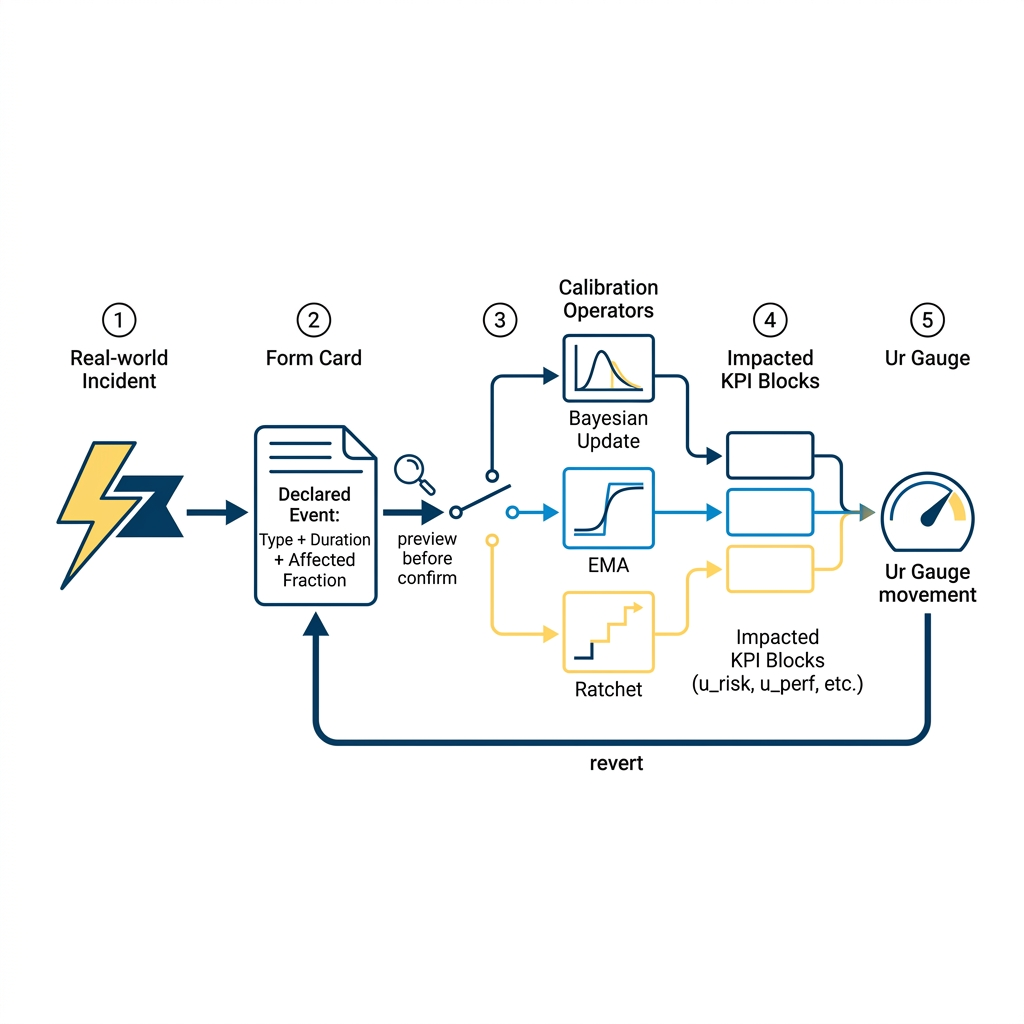
\includegraphics[width=0.85\linewidth]{Images/4.Operations/event_pipeline.png}
    \caption{From a declared event to a calibrated KPI update: the three calibration operators.}
    \label{fig:todraw_events}
\end{figure}

\begin{table}[H]
\centering
\caption{Component definitions for the event calibration operators.}
\label{tab:event_components}
\small
\begin{tabularx}{\linewidth}{llX}
\toprule
\textbf{Component} & \textbf{Type} & \textbf{Description} \\
\midrule
$p_{\text{post}}$ & Dependent variable & Revised failure probability after the event \\
$n_0$ & System parameter & Prior equivalent sample size ($26$, roughly six months) \\
$(k,n)$ & Event input & Equivalent failures/trials implied by the declared event's severity \\
$x_{\text{new}}$ & Dependent variable & Revised continuous KPI (e.g., availability) \\
$\lambda$ & System parameter & EMA reactivity weight, $\in[0.3,0.5]$ \\
\bottomrule
\end{tabularx}
\end{table}

\paragraph{Numerical Example: Strike Event.}
A node declares a \texttt{greve} (strike) lasting $d=24$~hours affecting a fraction $p_f=0.50$ of the workforce. Equivalent lost hours over a 168-hour week: $H_{\text{lost}} = d \times p_f = 12$, so $f_{\text{lost}} = 12/168 \approx 0.0714$ and the observed availability is $A_{\text{obs}} = 1 - 0.0714 \approx 0.9286$. Updating a baseline availability $A_{\text{old}}=0.95$ with EMA reactivity $\lambda=0.5$: $A_{\text{new}} = 0.5(0.95) + 0.5(0.9286) \approx 0.9393$. Risk severity is updated in ratchet mode: $S_{\text{new}} = \max(0.30, 0.50) = 0.50$. Operators can preview the transient impact of a declared event before confirming it, and reverting an event recomputes the baseline KPIs automatically.

The weekly cycle and event engine let coordinators keep the digital twin's KPI state current from structured, auditable inputs rather than free-form edits. This is what makes the resulting urgency history usable as a calibration dataset for the campaign of Section~\ref{sec:serious_game}.

%% ═══════════════════════════════════════════════════════════════════════════
\subsubsection{Explainability, Export, and Operational Hardening}
\label{sec:explain_export}
%% ═══════════════════════════════════════════════════════════════════════════

When the digital twin flags a node, the coordinator's first question is \emph{why}. The last three capabilities of the demonstrator exist to answer that question exactly, to let the data leave the tool, and to make sure nothing is ever lost.

\paragraph{Explainability.}
The per-node explanation page (\texttt{services/explain.py}) answers "why this score?" with exact decompositions, not approximations. Declared urgency splits into one additive contribution per AHP criterion, the same construction as Equation~\ref{eq:ud_local} read term by term:
\begin{equation}
    \kappa_j = w_j\,\frac{s_j-1}{8}, \qquad \sum_j \kappa_j = U_{d,\text{local}},
\end{equation}
so the page can state, for instance, that half of a node's declared urgency comes from the time-window criterion. Local real urgency splits the same way through the logarithm of Equation~\ref{eq:ur_local}: each block contributes $\ell_m = -\omega_m\ln(1-u_m)$, the block shares $c_m = \ell_m / \sum_k \ell_k$ sum to one, and $U_{r,\text{local}} = 1-\exp(-\sum_m \ell_m)$ reconstructs the score exactly. A coordinator can therefore see which block drives a node's urgency, and whether the gap between $U_d$ and $U_r$ is panic or hidden danger (Figure~\ref{fig:ponderation}).

\begin{figure}[H]
    \centering
    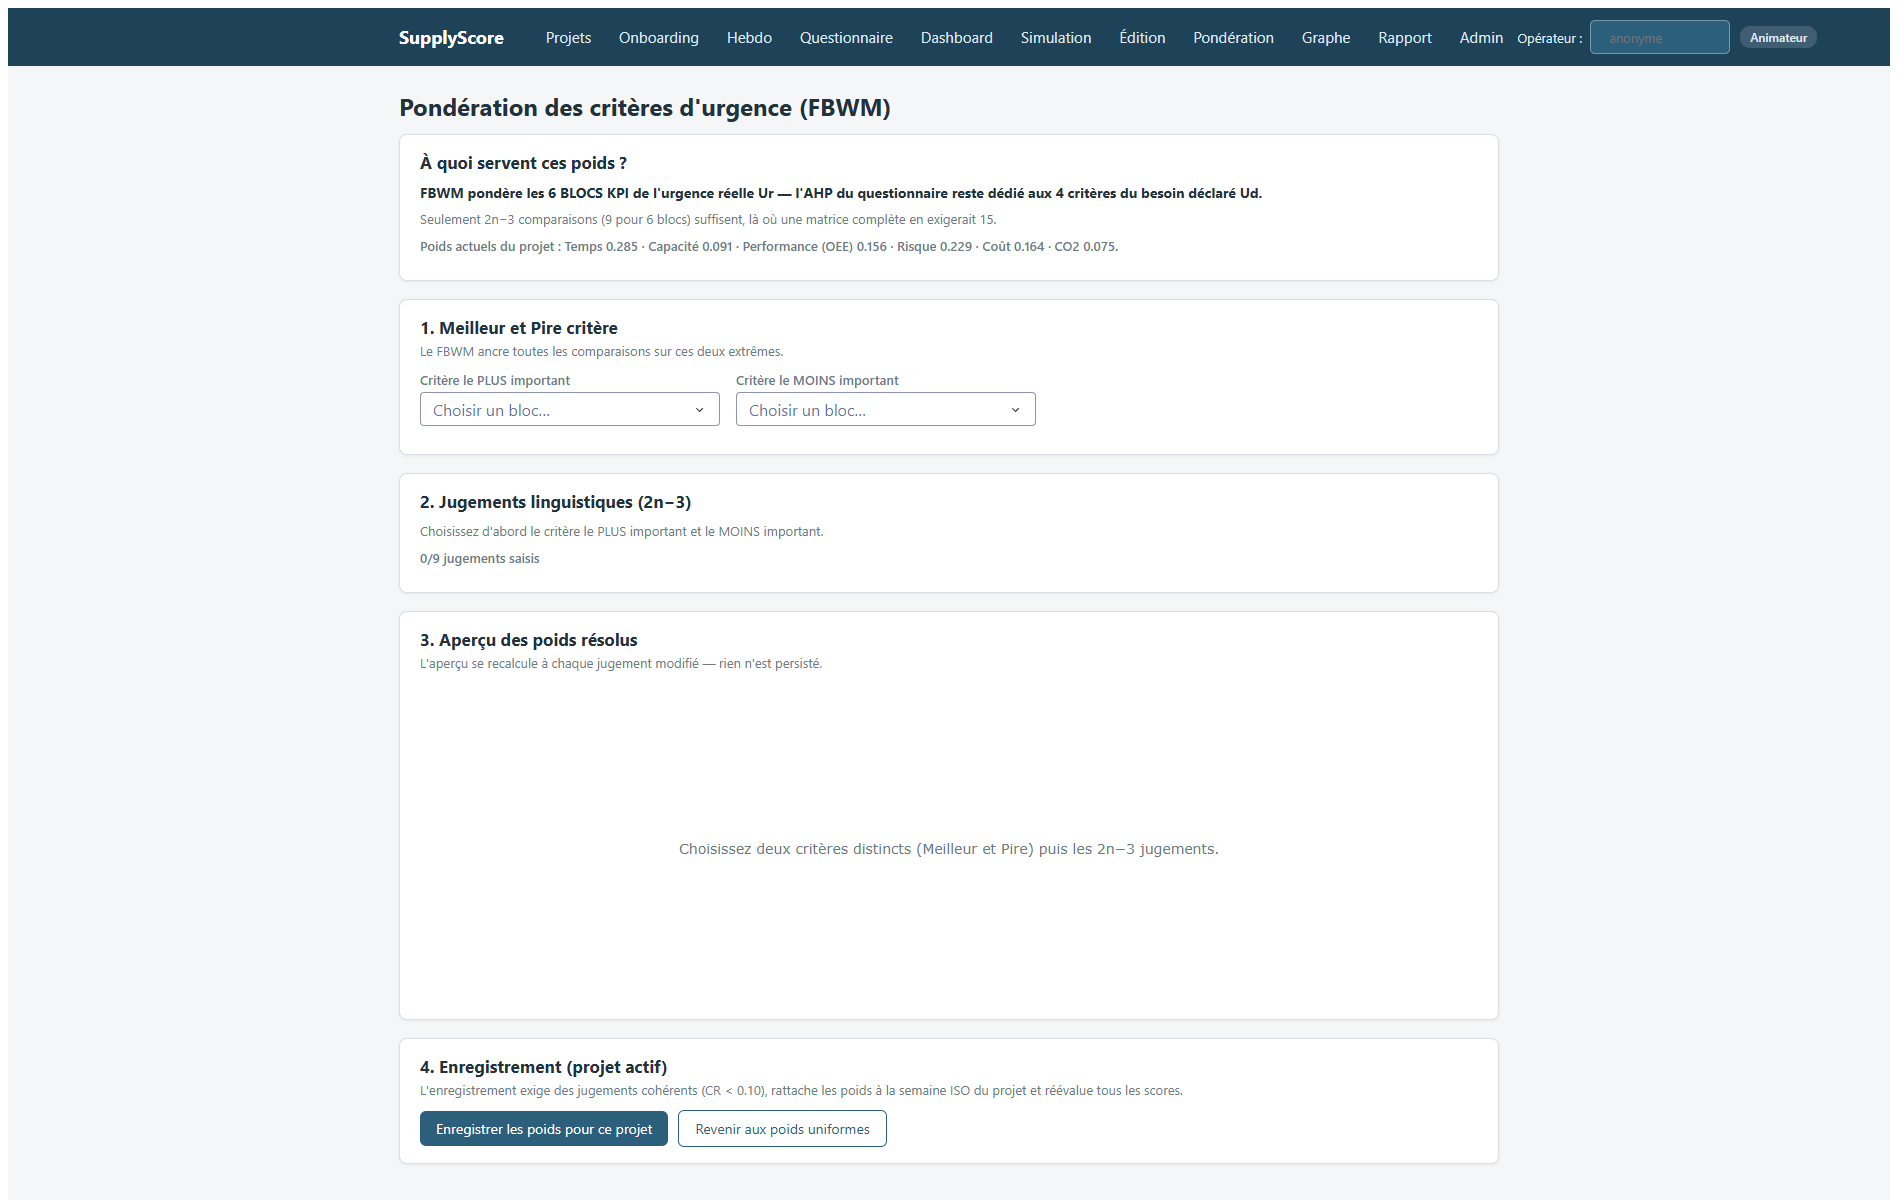
\includegraphics[width=0.85\linewidth]{Images/4.Operations/ponderation.png}
    \caption{Criteria weighting interface (Fuzzy-BWM) feeding the explainability decomposition.}
    \label{fig:ponderation}
\end{figure}

\begin{figure}[H]
    \centering
    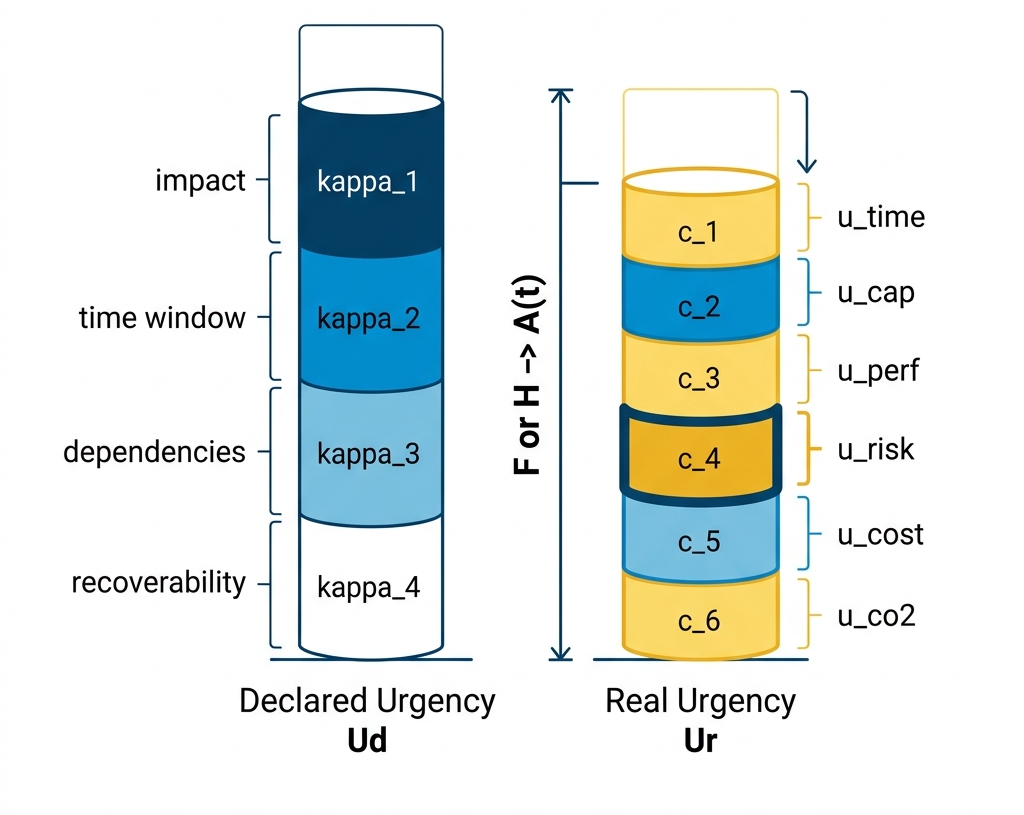
\includegraphics[width=0.85\linewidth]{Images/4.Operations/explainability_waterfall.png}
    \caption{Per-node explainability: exact additive decomposition of $U_d$ and $U_r$.}
    \label{fig:todraw_explain}
\end{figure}

\paragraph{Export.}
One action compiles the global registry and the per-node history into a twelve-worksheet Excel workbook (\texttt{services/exports.py}): project metadata, nodes, arcs, milestones, KPI history, urgency history, assessments, weekly reviews, KPI snapshots, events, decisions, and two audit-log sheets. All timestamps are converted to the coordinator's local timezone. Analyses can therefore run outside the tool, on frozen data, which the validation campaign relies on.

\paragraph{Operational Hardening.}
The persistence layer is SQLite, so data safety is handled explicitly (\texttt{data/}\allowbreak\texttt{backup.py}): Write-Ahead Logging is enabled, an integrity check runs before every backup, and the native \texttt{sqlite3.backup} API copies each database without locking the running application. Automatic backups run every 24 hours with a retention cap of 20 archives, and schema migrations are versioned (Figure~\ref{fig:admin}).

\begin{figure}[H]
    \centering
    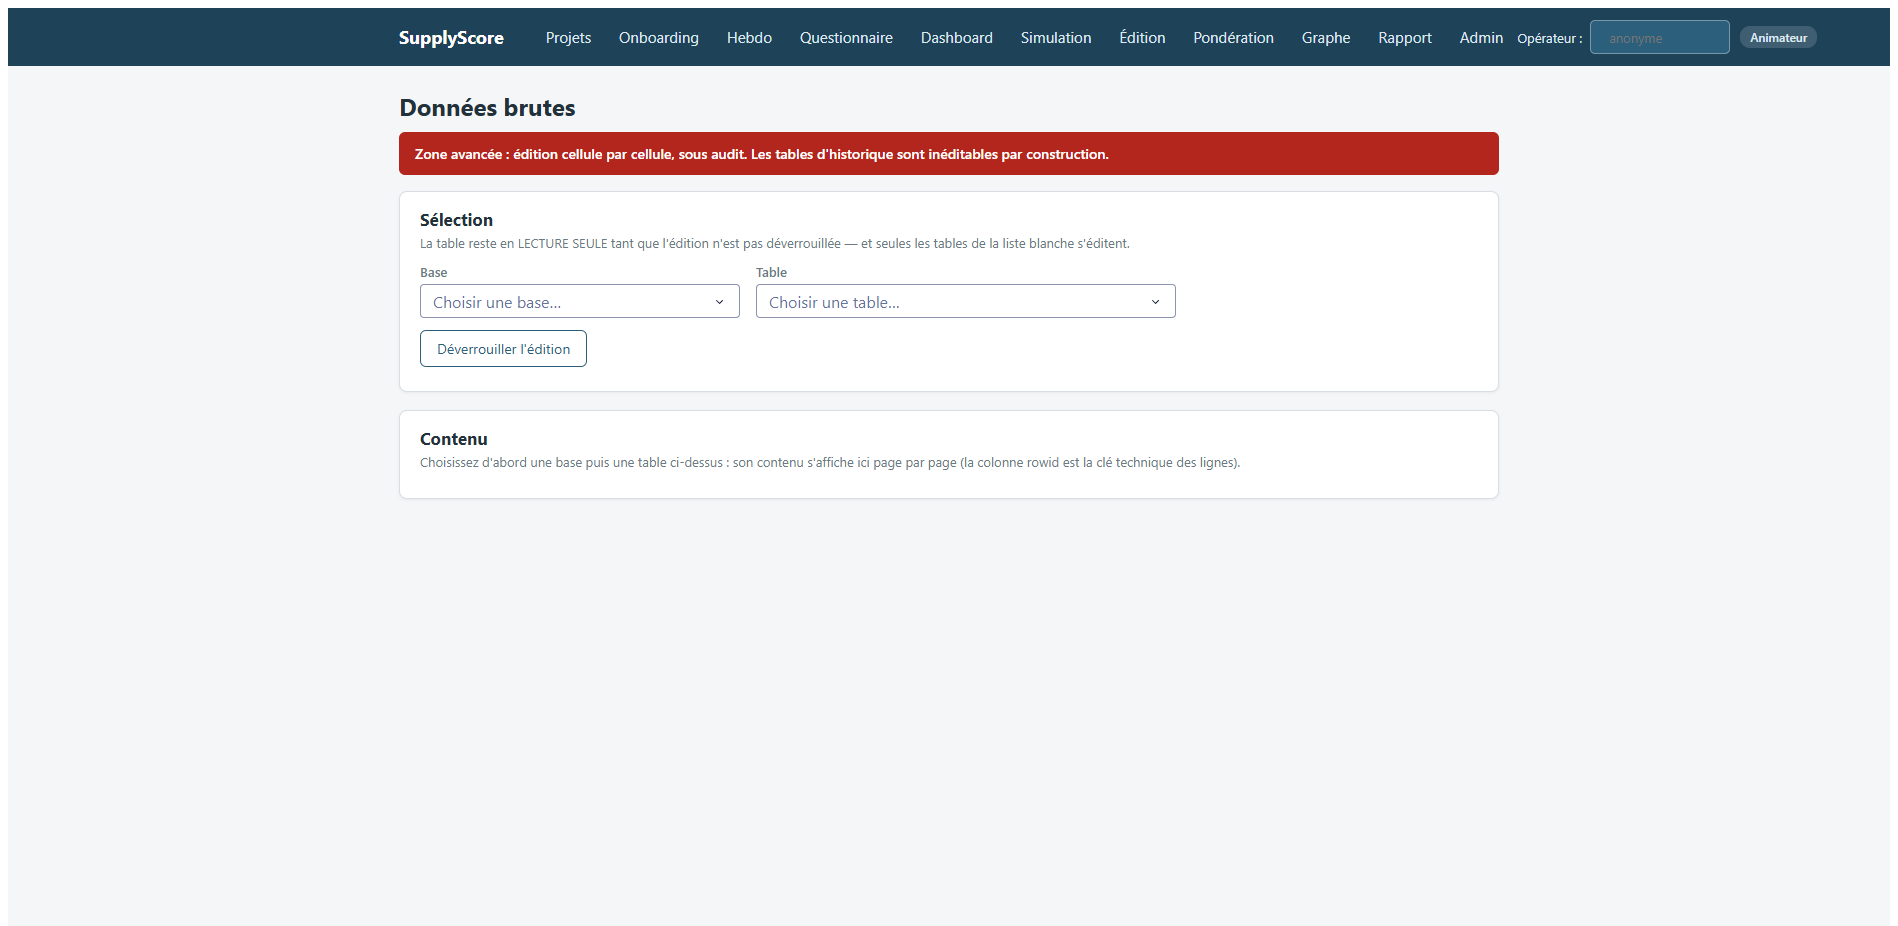
\includegraphics[width=0.85\linewidth]{Images/4.Operations/admin.png}
    \caption{Administration page: database sizes, migration version, and backup controls.}
    \label{fig:admin}
\end{figure}

These three capabilities are not peripheral. They are what make the adequacy score auditable and the digital twin operable outside a development environment, and they are preconditions for the campaign below.

%% ═══════════════════════════════════════════════════════════════════════════
\subsection{Use Case and Validation: The HÉLIOS Serious-Game Campaign}
\label{sec:serious_game}
%% ═══════════════════════════════════════════════════════════════════════════

Everything up to this point establishes that the model is implemented, internally consistent, and tested. What it does not establish is whether the adequacy signal says anything true about real operators facing a real crisis. This section presents the validation campaign built for that purpose: its design, its current state of readiness, and what has been learned from the two checks already run against it. The campaign replays the 2020--2022 semiconductor shortage as a serious game, designed, calibrated through five dry runs, and pre-registered before execution.

\paragraph{Campaign Design.}
The campaign, presented to participants under the cover story \emph{Programme HÉLIOS}, replays the semiconductor crisis over 18 weekly game turns compressed into nine working days (two turns per day, morning and late afternoon). Those 18 playing turns follow an opening turn on which the first declarations are made, so a run is indexed T0 to T18 and every result in this section counts nineteen turns; the two figures describe the same campaign. The supply network has eight nodes, one per consultant, anchored on the real actor types of the crisis (Table~\ref{tab:helios_network}).

\begin{table}[H]
\centering
\caption{The eight HÉLIOS campaign nodes and their real-world anchors.}
\label{tab:helios_network}
\small
\begin{tabularx}{\linewidth}{>{\raggedright\arraybackslash}p{3.1cm} >{\raggedright\arraybackslash}p{2.6cm} c X}
\toprule
\textbf{Node} & \textbf{Role} & \textbf{Rank} & \textbf{Real-world anchor} \\
\midrule
Orbitalys & Satellite prime, final customer & 0 & Fictional satellite programme, contractual delivery pressure \\
AvioSys Int\'egration & Avionics integrator & 1 & Qualified-stock squeeze on avionics tier-1 suppliers \\
\'Electis EMS & Electronics manufacturing services & 2 & EMS plants placed under allocation, 2021 \\
CompoDis Europe & Component distributor & 3 & Distributor allocation and spot-market premiums \\
TransGlobal Fret & Freight operator & 3 & Suez Canal blockage, West Coast port congestion \\
NovaFab Semiconductors & Foundry, expected bottleneck & 4 & Composite of the Texas winter-storm freeze and the Taiwan drought \\
Meridian Semi & Secondary foundry, inert backup arc & 4 & A foundry sold out through 2023: the announced "plan B" that delivers nothing \\
SilPure Materials & Raw wafer supplier & 5 & Roughly 60\% of world wafer supply; polysilicon price roughly tripling in 2021 \\
\bottomrule
\end{tabularx}
\end{table}

\begin{figure}[H]
    \centering
    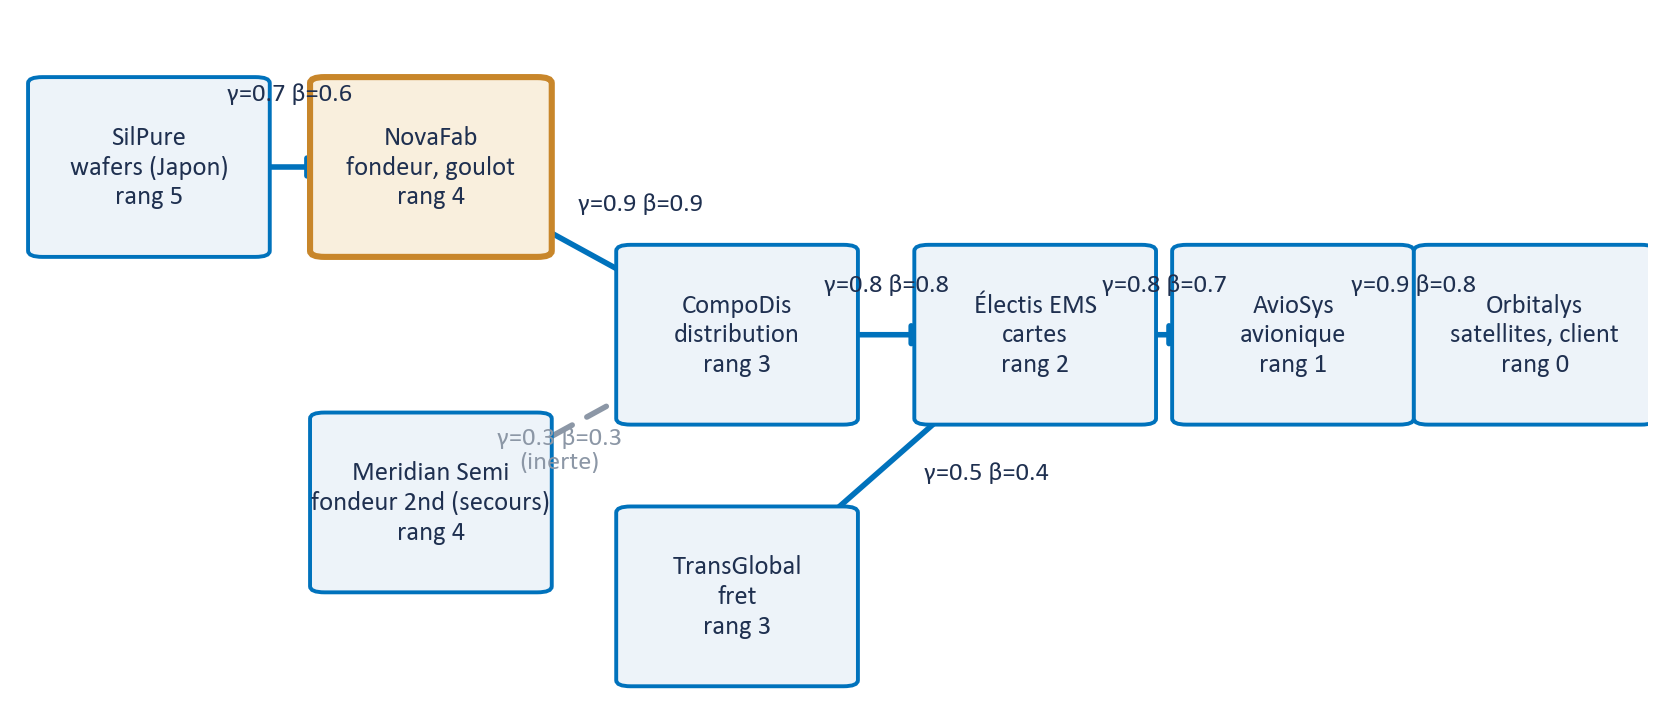
\includegraphics[width=\linewidth]{Images/4.Operations/helios_network_coefficients.png}
    \caption{The HÉLIOS network with its per-arc coefficients: $\gamma$ (downstream demand attenuation) and $\beta$ (upstream risk amplification), and each node's tier rank. NovaFab (rank 4) is the expected bottleneck; the dashed Meridian arc is the inert backup arc of Section~\ref{sec:math_framework}.}
    \label{fig:helios_network_coefficients}
\end{figure}

The eighteen turns follow five acts drawn from the documented chronology of the real crisis: a baseline where early warning signs go unheeded (turns 1--4), a tipping point where a foundry freeze, a competitor fire, and a canal blockage make the crisis visible (turns 5--8), a squeeze where spot prices reach ten to forty times catalogue and no node keeps any margin (turns 9--12), a rupture where a major manufacturer cuts production by roughly 40\%, the bullwhip effect takes hold, and the announced backup foundry turns out to have no spare capacity (turns 13--16), and a slow, partial recovery that measures whether declared urgency lags the physical de-escalation (turns 17--18).

Each act is driven by calibrated engine events whose type, parameters, and timing are taken from that chronology; the twelve events are listed in Table~\ref{tab:helios_events}. One game turn represents one real month, from September 2020 to February 2022, with real durations converted into engine hours at a fixed rate (one real week maps to roughly 38.7 engine hours), so that documented figures such as the twelve-to-twenty-five-week supplier lead times or the six-day canal blockage keep their true magnitude inside an eighteen-turn game.

\begin{table}[H]
\centering
\caption{The twelve calibrated engine events that drive the HÉLIOS crisis, with their real-world anchors.}
\label{tab:helios_events}
\small
\begin{tabularx}{\linewidth}{c >{\raggedright\arraybackslash}p{2.3cm} >{\raggedright\arraybackslash}p{2.9cm} X}
\toprule
\textbf{Turn} & \textbf{Node} & \textbf{Event type} & \textbf{Real-world anchor} \\
\midrule
T3 & NovaFab & Demand spike & Automotive reorders on sold-out slots, Nov.\ 2020 \\
T5 & CompoDis & Supplier delay & Distributor moves to allocation, Jan.\ 2021 \\
T6 & NovaFab & Accident (critical) & Texas winter-storm fab freeze, Feb.\ 2021 \\
T7 & NovaFab & Demand spike & Reorders after a competitor's fab fire, Mar.\ 2021 \\
T7 & TransGlobal & Transport disruption & Suez Canal blockage, six days, Mar.\ 2021 \\
T10 & NovaFab & Material shortage & Taiwan drought, ultrapure-water rationing, Jun.\ 2021 \\
T12 & \'Electis & Capacity loss & Southeast-Asia backend lockdowns, Aug.\ 2021 \\
T12 & TransGlobal & Transport disruption & Shift to saturated air freight, Aug.\ 2021 \\
T13 & CompoDis & Demand spike & Bullwhip over-ordering, Sep.\ 2021 \\
T14 & TransGlobal & Transport disruption & West Coast port congestion, Oct.\ 2021 \\
T14 & CompoDis & Tariff increase & Allocation spot premiums, Oct.\ 2021 \\
T16 & SilPure & Tariff increase & Polysilicon price pass-through, Dec.\ 2021 \\
\bottomrule
\end{tabularx}
\end{table}

One encoding choice is worth noting. The Texas freeze is modelled as a production accident, which triggers the engine's Bayesian revision of the failure probability, a recovery clock, and a severity ratchet, rather than as a capacity loss, which would only reduce storage volume: a hot shutdown of a fabrication line is mechanically closer to the former.

The two urgency signals come from different worlds, which is the point of the design. Real urgency $U_r$ is fed from public time series of the actual crisis (INSEE production and price indices, WSTS worldwide semiconductor billings, and a Kaggle semiconductor-shortage dataset), frozen in a data pack whose SHA-256 hashes were recorded before the first turn. Every third-party dataset is passed through an authenticity check before use: a Kaggle logistics dataset initially considered for the freight node was rejected at this check for the signatures of synthetic training data (pre-computed target columns, GPS coordinates scattered outside the region the dataset claimed to cover, uniformly flat distributions), while the semiconductor-shortage dataset passed (a secular price decline, a genuine 2021 upturn, sectoral employment consistent with official series) and was kept. The rejected dataset is retained in the raw-data folder for audit but is never loaded by the analysis pipeline; the freight node's cost block is instead driven entirely by the calibrated events of Section~\ref{sec:weekly_cycle}. Declared urgency $U_d$ comes from the consultants through the same weekly AHP questionnaire described in Section~\ref{sec:ahp_tool}, under ten minutes per turn, with the consistency gate active.

Two data-provenance rules protect the real-urgency series. First, a single-pilot rule forbids double counting: each KPI field of each node is driven either by a time series or by a calibrated event, never by both, so when an event writes a field on a given turn the series skips that turn. Second, one honest artefact of the real data is kept rather than smoothed away. The INSEE business-failures series falls through 2020 and 2021, under public support schemes, so a failure-rate indicator taken alone would lower external risk exactly while the sector crisis was worsening. Keeping it is the multi-block argument made concrete: a single macroeconomic indicator can tell the opposite of the ground truth, which is why real urgency aggregates six blocks rather than trusting one.

\begin{figure}[H]
    \centering
    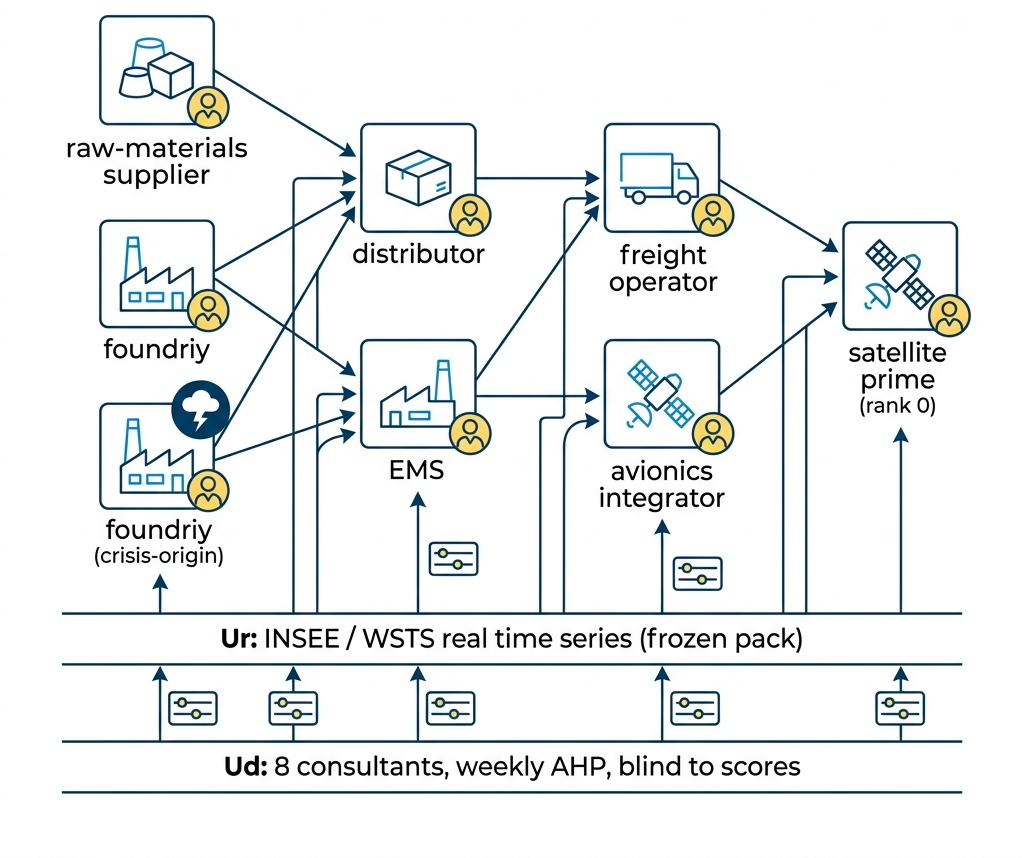
\includegraphics[width=0.85\linewidth]{Images/4.Operations/campaign_network.png}
    \caption{The eight-node HÉLIOS campaign network. The person icon on each node marks the consultant who plays it, feeding $U_d$ through the weekly AHP questionnaire; the lower band shows the public data series that independently feed $U_r$.}
    \label{fig:todraw_campaign}
\end{figure}

\paragraph{Protocol Integrity.}
The experimental protocol was frozen before the first real turn. Consultants see only their own role sheet and the questionnaire page; dashboards and scores stay hidden until the debrief. No discussion between roles is allowed during the campaign. Two placebo sheets, a false de-escalation handed to the avionics integrator at turn 9 and to the wafer supplier at turn 15, control for suggestibility: if a consultant's declared urgency follows the placebo, the measure is reflecting the sheet handed to them rather than a memory of the real crisis. A weak-signal turn (turn 4), where the press mentions a tension with no engine event behind it, measures who reacts to media noise alone. Every deviation from protocol is logged the same day in a campaign journal. Two further safeguards protect internal validity: roles are assigned so that the two most information-heavy nodes, the foundry and the distributor, do not go to the most supply-chain-experienced consultants, keeping a role effect from being confounded with an expertise effect, and at the debrief each consultant is asked at which turn they recognised the real crisis, which turns the main threat to a blind declaration into a measured quantity rather than an uncontrolled one. The hypothesis register is the one of Section~\ref{sec:hypotheses}: H1 to H6, each with a numeric threshold fixed in advance, so that success and failure are defined before the data exists. Any analysis outside that register is labelled exploratory.

\paragraph{Empirical Calibration of the Adequacy Signal.}
The campaign feeds the calibration service (\texttt{services/calibration.py}), which addresses Challenge~3 (Section~\ref{sec:locks}) and hypotheses H2 and H4: does the hidden-risk signal $H$ have predictive value beyond a raw KPI threshold? For each recorded (node, week) pair, the historical hidden risk is compared against negative outcomes observed in a subsequent four-week window (a missed milestone, an abandoned node, or a critical event). The resulting confusion matrix yields precision, recall, and F1:
\begin{equation}
    \text{Precision} = \frac{TP}{TP+FP}, \qquad \text{Recall} = \frac{TP}{TP+FN}, \qquad F1 = \frac{2 \times \text{Precision}\times\text{Recall}}{\text{Precision}+\text{Recall}}.
    \label{eq:calib_metrics}
\end{equation}

\paragraph{Mechanical Validation: The Synthetic Dry Run.}
Before any human data exists, the full campaign mechanics were exercised end to end on a disposable database: five iterations (v1 to v5) calibrated the scenario and eliminated engine artefacts, and the final iteration replayed all nineteen turns (T0 to T18) with synthetic respondents standing in for the eight consultants. This dry run is an engineering check, not a scientific one: the synthetic declared urgency is anchored directly on each node's own local real urgency ($1 + 8 \times U_{r,\text{local}}$, perturbed by a fixed panic, under-report, or neutral bias per role), so it cannot lag its own physical signal, cannot under-report it for long, and cannot over-react to a press event it does not read. Run against the pre-registered tests, the dry run therefore returns not confirmed or not applicable on all six hypotheses by construction (Table~\ref{tab:helios_dryrun}), which is the expected and informative outcome: it confirms that the full pipeline, injection, weekly decay, milestone drift, event calibration, propagation, criticality, snapshotting, and backup, runs correctly under the two-turn-per-day cadence the real campaign requires, and it calibrated the null-baseline detector (a raw threshold $U_{r,\text{local}} \ge 0.5$) at precision $0.16$ and recall $0.27$: the bar the hidden-risk signal must clear in the real campaign to demonstrate added value beyond a raw KPI reading (Challenge~3, Section~\ref{sec:locks}).

\begin{table}[H]
\centering
\caption{Dry-run v5 verdicts on synthetic data: an engineering check, not a hypothesis test.}
\label{tab:helios_dryrun}
\small
\begin{tabularx}{\linewidth}{>{\raggedright\arraybackslash}p{3.4cm} >{\raggedright\arraybackslash}p{2.4cm} X}
\toprule
\textbf{Test} & \textbf{Verdict} & \textbf{Measured value} \\
\midrule
H1 latency & Not confirmed & 1 of 8 nodes at lag $\ge 1$ turn (threshold: 5 of 8) \\
H2 early detection & Not confirmed & $H(\text{NovaFab})$ peaks at $0.070$ on turns 6--12 (threshold: $0.3$) \\
H3 criticality & Not confirmed & NovaFab top-1 on 7 of 10 informative turns, $70\%$ (threshold: $80\%$; saturated turns excluded, Section~\ref{sec:criticality}) \\
H4 predictive validity & Not confirmed & precision $0.00$, recall $0.00$ at $H \ge 0.5$ (threshold: $0.5$; null baseline: precision $0.16$, recall $0.27$) \\
H5 contagion & Not confirmed & non-affected nodes: $\Delta U_d = -0.007$ on press turns vs.\ $+0.031$ on calm turns \\
H6 hysteresis & Not applicable & real urgency shows no measurable decline over the recovery turns, so the comparison is not meaningful \\
\bottomrule
\end{tabularx}
\end{table}

Figure~\ref{fig:helios_dryrun_trajectories} shows why: for every one of the eight nodes, real urgency (solid) and synthetic declared urgency (dashed) track each other closely across the full replay, rather than one lagging or decoupling from the other. That closeness is the visual signature of the circularity described above, not a property the real campaign is expected to reproduce. Table~\ref{tab:helios_trajectories} traces the same propagated real urgency at eight representative turns, showing the crisis propagate through the network broadly as the scenario intends: a slow build in the baseline, the sharp T6--T8 tipping point at NovaFab, TransGlobal, and CompoDis, a saturated network through the squeeze and rupture, and a partial, uneven recovery where NovaFab barely eases while Meridian, hit late by the worldwide demand wave, saturates only at the very end.

\begin{figure}[H]
    \centering
    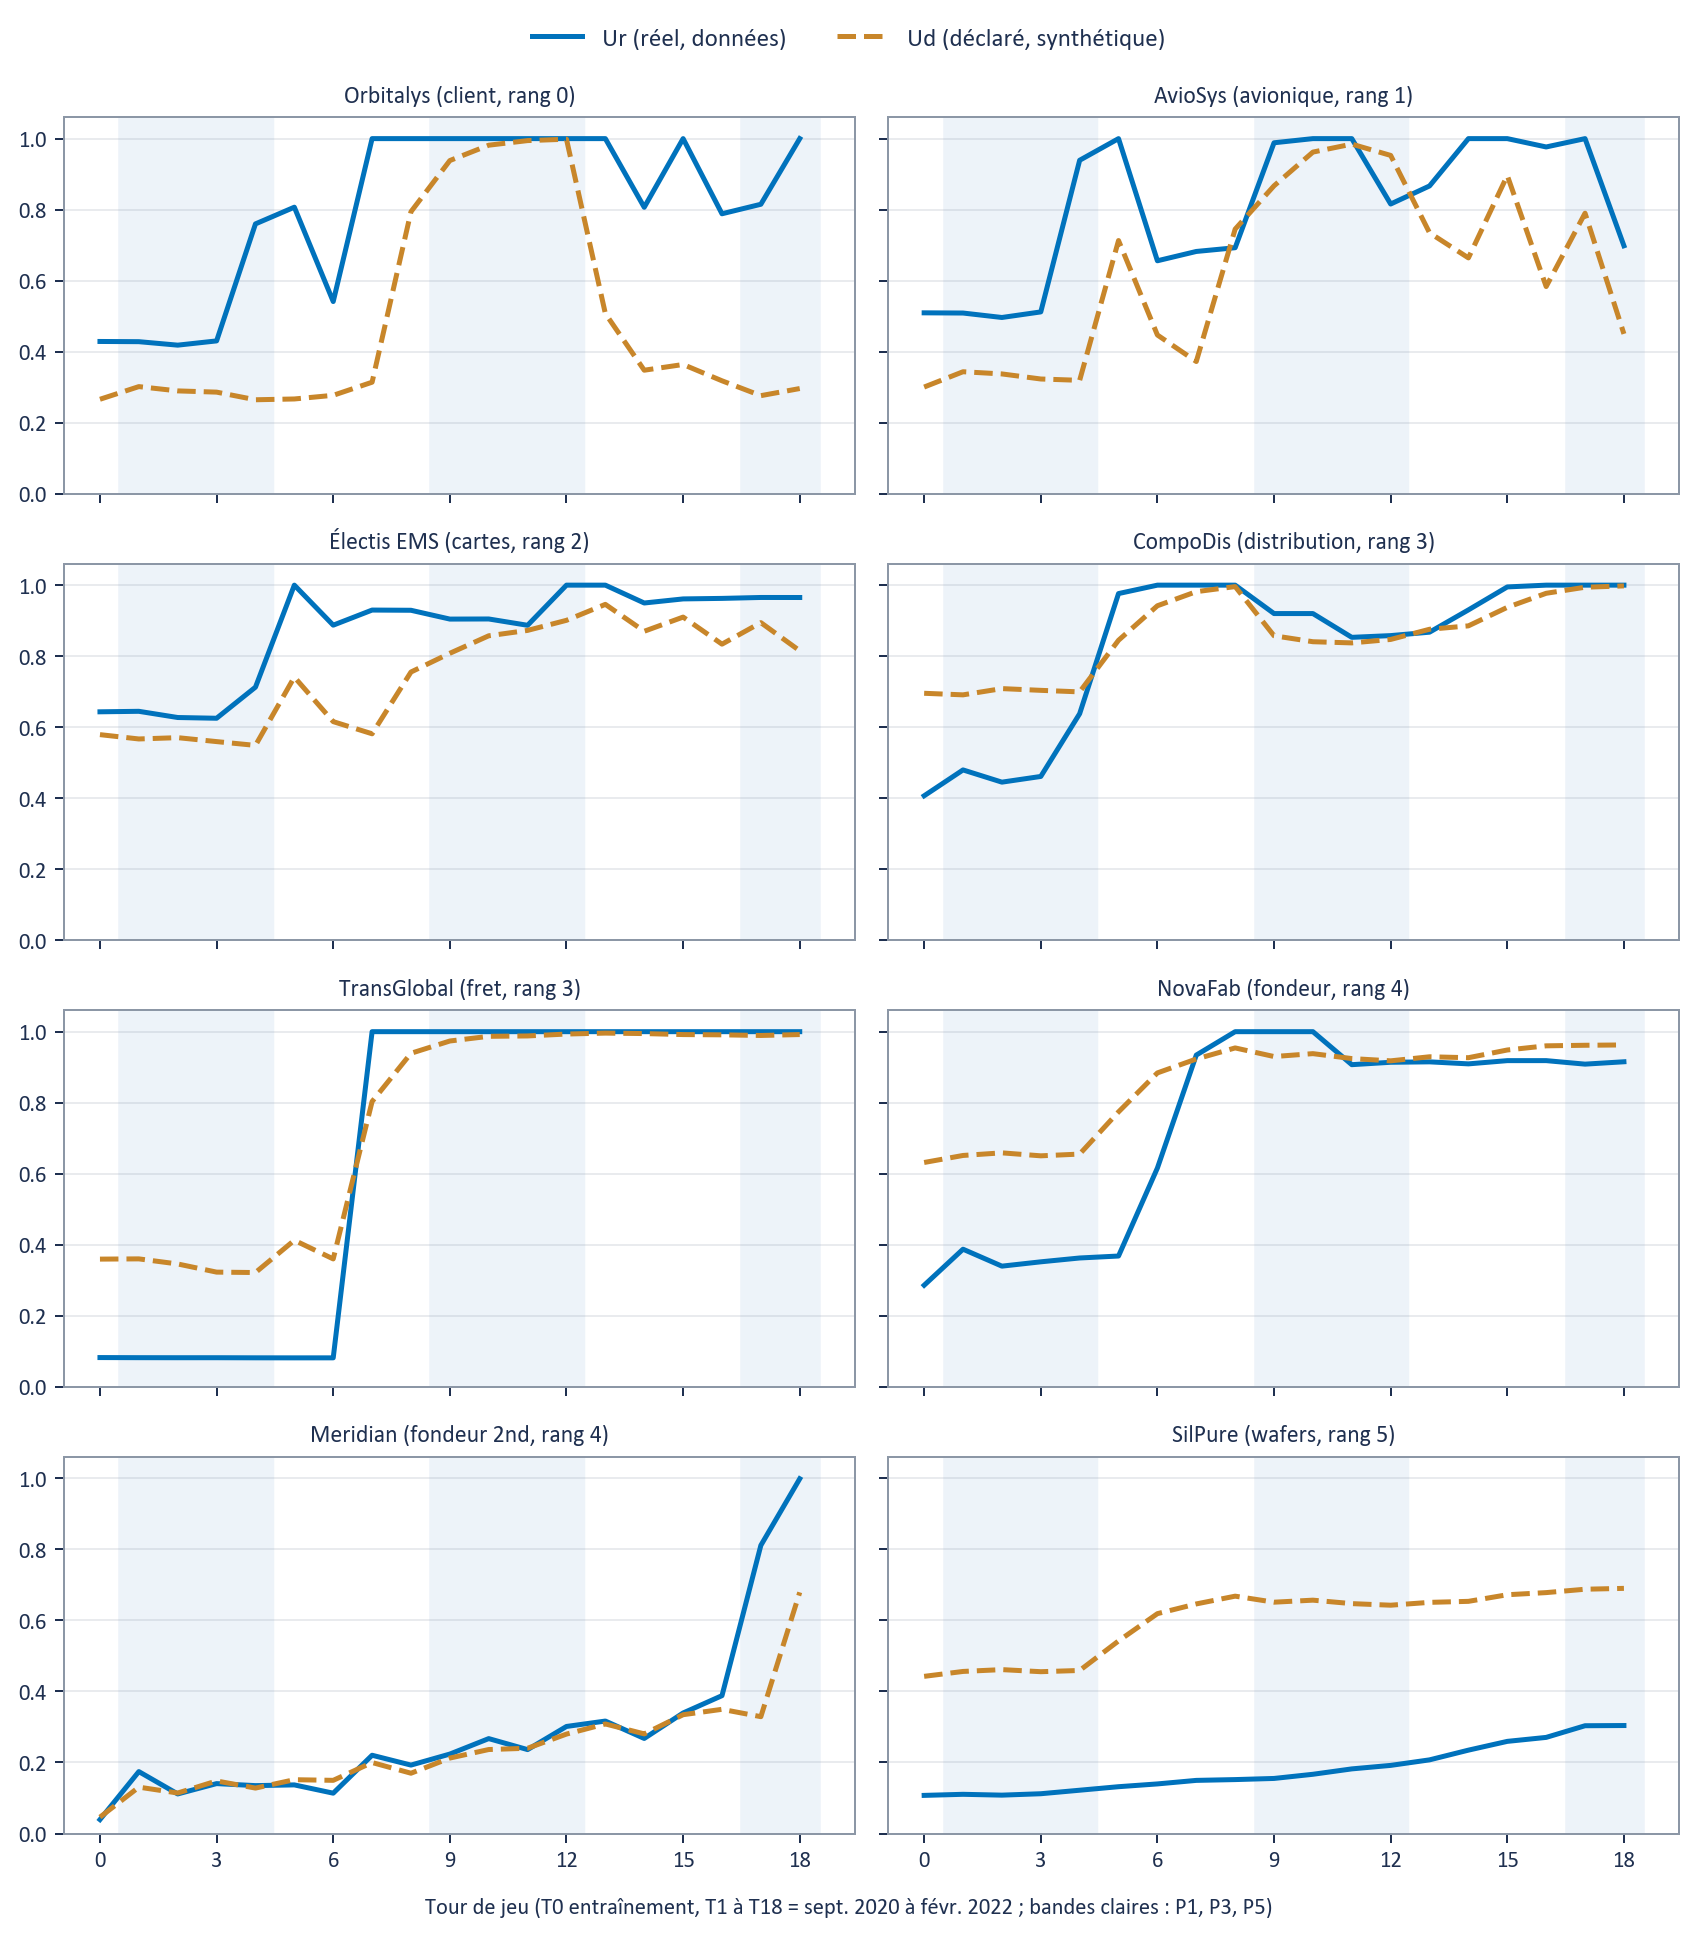
\includegraphics[width=0.85\linewidth]{Images/4.Operations/helios_dryrun_trajectories.png}
    \caption{Real urgency $U_r$ (solid) against synthetic declared urgency $U_d$ (dashed) for all eight nodes across the dry-run v5 replay (T0 to T18, shaded bands mark phases P1, P3, P5). The synthetic $U_d$ follows $U_r$ at every node by construction, which is why H1, H2, H5, and H6 are not interpretable on this run.}
    \label{fig:helios_dryrun_trajectories}
\end{figure}

\begin{table}[H]
\centering
\caption{Propagated real urgency $U_r$ by node across the dry-run v5 replay (selected turns).}
\label{tab:helios_trajectories}
\small
\begin{tabularx}{\linewidth}{l >{\centering\arraybackslash}X >{\centering\arraybackslash}X >{\centering\arraybackslash}X >{\centering\arraybackslash}X >{\centering\arraybackslash}X >{\centering\arraybackslash}X >{\centering\arraybackslash}X >{\centering\arraybackslash}X}
\toprule
\textbf{Node} & T0 & T4 & T6 & T8 & T10 & T13 & T16 & T18 \\
\midrule
Orbitalys & 0.43 & 0.76 & 0.54 & 1.00 & 1.00 & 1.00 & 0.79 & 1.00 \\
AvioSys & 0.51 & 0.94 & 0.66 & 0.69 & 1.00 & 0.87 & 0.98 & 0.70 \\
\'Electis & 0.64 & 0.71 & 0.89 & 0.93 & 0.90 & 1.00 & 0.96 & 0.97 \\
CompoDis & 0.41 & 0.64 & 1.00 & 1.00 & 0.92 & 0.87 & 1.00 & 1.00 \\
TransGlobal & 0.08 & 0.08 & 0.08 & 1.00 & 1.00 & 1.00 & 1.00 & 1.00 \\
NovaFab & 0.29 & 0.36 & 0.62 & 1.00 & 1.00 & 0.92 & 0.92 & 0.92 \\
Meridian & 0.04 & 0.13 & 0.11 & 0.19 & 0.27 & 0.32 & 0.39 & 1.00 \\
SilPure & 0.11 & 0.12 & 0.14 & 0.15 & 0.17 & 0.21 & 0.27 & 0.30 \\
\bottomrule
\end{tabularx}
\end{table}

The confusion matrix behind the H4 row of Table~\ref{tab:helios_dryrun} is given in full in Table~\ref{tab:helios_calibration}, since it is what the real campaign's confusion matrix will be measured against.

\begin{table}[H]
\centering
\caption{Calibration confusion matrix on the dry-run v5 synthetic replay (152 node-turn observations).}
\label{tab:helios_calibration}
\small
\begin{tabularx}{\linewidth}{lX}
\toprule
\textbf{Quantity} & \textbf{Value} \\
\midrule
True positives / false positives (hidden-risk signal, $H \ge 0.5$) & 0 / 5 \\
True negatives / false negatives (hidden-risk signal, $H \ge 0.5$) & 102 / 37 \\
Precision / recall, hidden-risk signal & $0.00$ / $0.00$ \\
Precision / recall, null baseline ($U_{r,\text{local}} \ge 0.5$) & $0.16$ / $0.27$ \\
\bottomrule
\end{tabularx}
\end{table}

\begin{figure}[H]
    \centering
    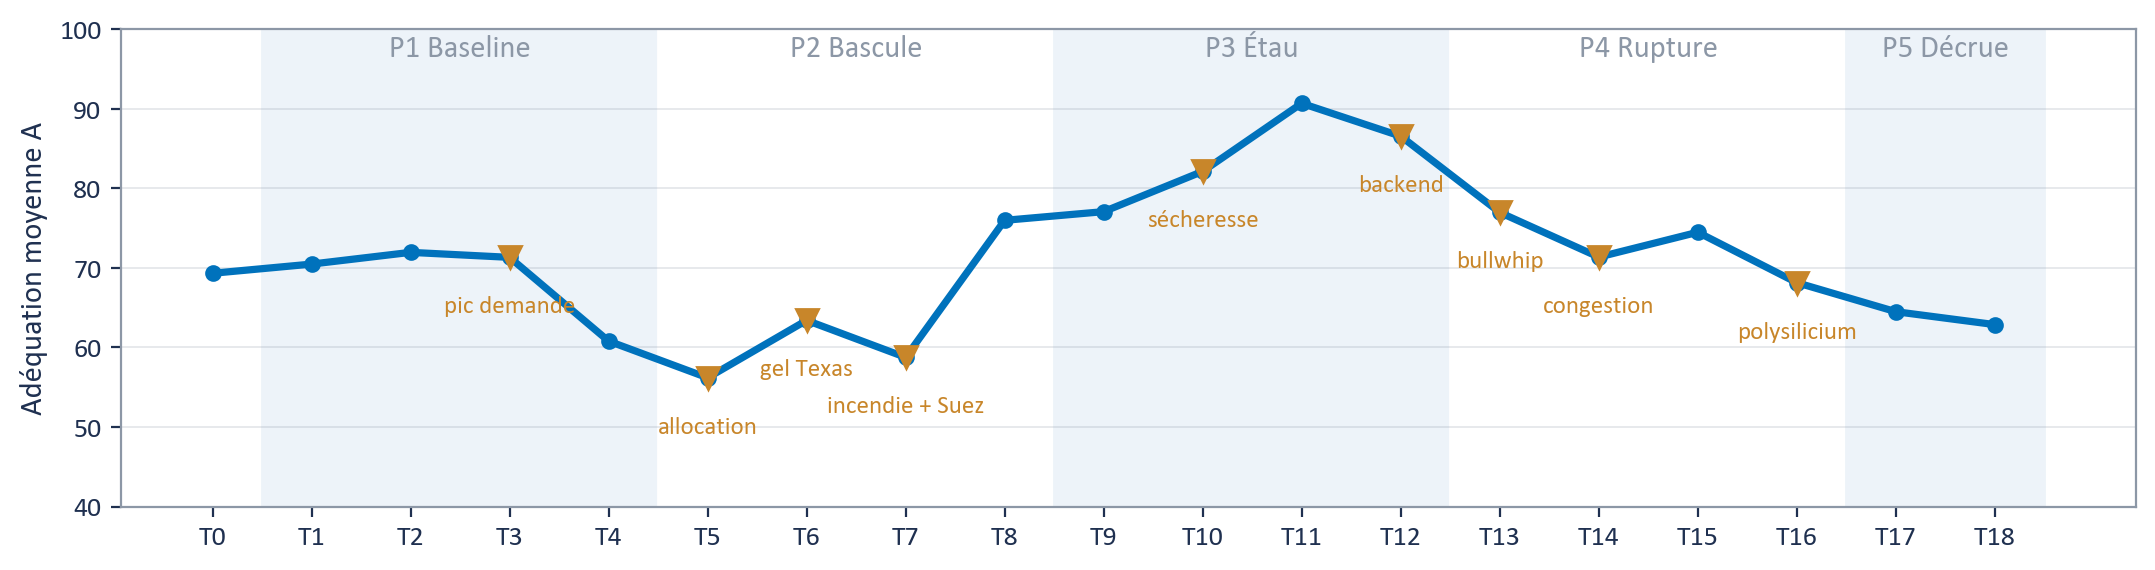
\includegraphics[width=0.85\linewidth]{Images/4.Operations/helios_dryrun_adequacy.png}
    \caption{Network-average adequacy score $A$ across the dry-run v5 replay, annotated with the scenario's calibrated events. The score falls sharply at fast turning points (demand spike, Texas freeze, fire and Suez, drought), then rises through the squeeze (P3) as the saturated network is uniformly tracked by the synthetic $U_d$, before eroding again as the bullwhip and congestion events land.}
    \label{fig:helios_dryrun_adequacy}
\end{figure}

\paragraph{Exploratory Pilot: Eight Isolated Language-Model Agents.}
A second, more informative pilot replaced the fixed-bias synthetic generator with eight isolated large-language-model agents, one per role, each confined to its own role card and turn briefings, with no access to the other roles, the dashboard, or future turns, the same anti-lookahead discipline required of the real consultants. Each agent read its briefing in character and answered the real AHP tool of Section~\ref{sec:ahp_tool}, pairwise comparisons and severity scores through the production consistency-ratio code. Unlike the synthetic dry run, this pilot exercised the full production pipeline rather than a standalone computation: campaign setup, turn injection, and questionnaire submission all ran through the same weekly-cycle service (\texttt{services/orchestrator.py}) that a browser-based consultant reaches, closing on the same live dashboard built for the real campaign. This pilot is exploratory: it was not part of the pre-registered protocol, and a single language-model instance per role has no statistical standing as a substitute for eight independent human judges. Table~\ref{tab:helios_llm_pilot} gives its verdicts on the same six pre-registered tests.

\begin{table}[H]
\centering
\caption{LLM-pilot verdicts: eight isolated language-model agents replaying the real AHP questionnaire through the production pipeline (exploratory, not pre-registered).}
\label{tab:helios_llm_pilot}
\small
\begin{tabularx}{\linewidth}{>{\raggedright\arraybackslash}p{3.4cm} >{\raggedright\arraybackslash}p{2.4cm} X}
\toprule
\textbf{Test} & \textbf{Verdict} & \textbf{Measured value} \\
\midrule
H1 latency & Not confirmed & 3 of 8 nodes at lag $\ge 1$ turn (threshold: 5 of 8) \\
H2 early detection & Not confirmed & $H(\text{NovaFab})$ peaks at $0.017$ on turns 6--12 (threshold: $0.3$) \\
H3 criticality & Not confirmed & NovaFab top-1 on 7 of 10 informative turns, $70\%$ (threshold: $80\%$; identical to the dry run, a $U_d$-independent test) \\
H4 predictive validity & Not confirmed & precision $0.00$, recall $0.00$ at $H \ge 0.5$ ($TP=0$, $FP=2$, $TN=105$, $FN=37$) \\
H5 contagion & Confirmed & non-affected nodes: $\Delta U_d = +0.079$ on press turns vs.\ $+0.005$ on calm turns \\
H6 hysteresis & Not applicable & real urgency shows no measurable decline over the recovery turns \\
\bottomrule
\end{tabularx}
\end{table}

Two results stand out. The urgency-contagion hypothesis (H5) is confirmed: declared urgency of non-affected nodes rises by $0.079$ on press-event turns against $0.005$ on calm turns, matching the pre-registered direction and ordering. The latency hypothesis (H1) moves from 1 of 8 nodes on the synthetic dry run to 3 of 8 nodes at a lag of one turn or more, closer to, but still short of, the pre-registered threshold of 5. Both results are a first sign of a non-circular declared-urgency signal: a reasoning-based judge, unlike the dry run's formula, can in principle lag or amplify the physical signal instead of tracking it by construction. H4 stays not confirmed, but for a specific and informative reason: these agents read their briefing carefully and declared urgency close to what the briefing in fact described, so their $U_d$ tracks $U_r$ too closely to leave the gap that $H$ is built to catch, an even tighter tracking than the fixed-bias dry run ($H(\text{NovaFab})$ peaks at $0.017$ against $0.070$). H3 is unchanged from the dry run because it depends only on the network's real-urgency criticality ranking, not on $U_d$ at all. H6 stays not applicable for the same reason as the dry run: real urgency shows no measurable decline over the recovery turns. Taken together, this pilot motivates, without yet establishing, the idea that a genuinely reasoning-based declared-urgency signal can decouple from the physical signal in the way the model's hypotheses predict, and it sharpens rather than removes the case for the real campaign: only a human's imperfect, potentially under-reporting perception of a crisis, not a careful reader's, can put H4 to a fair test.

\paragraph{The Pilot's Final Application State.}
The pilot did not just produce six hypothesis verdicts: it left behind a live SupplyScore project, reloadable in the same dashboard a coordinator would use in production. Read directly from that project after the eighteenth turn, the network-average adequacy is $65.5$, four of the eight nodes carry a hidden-risk reading above $0.1$, one carries a false-urgency reading above $0.1$, and the single worst-scoring node by a wide margin is Orbitalys at $A=15.3$; Table~\ref{tab:llm_pilot_snapshot} lists the full per-node snapshot.

\begin{table}[H]
\centering
\caption{Final per-node snapshot of the LLM pilot's SupplyScore project, read directly from the application after turn 18.}
\label{tab:llm_pilot_snapshot}
\small
\begin{tabularx}{\linewidth}{l >{\centering\arraybackslash}X >{\centering\arraybackslash}X >{\centering\arraybackslash}X >{\centering\arraybackslash}X >{\centering\arraybackslash}X}
\toprule
\textbf{Node} & $U_d$ & $U_r$ & $A$ & $F$ & $H$ \\
\midrule
Orbitalys & 0.409 & 1.000 & 15.3 & 0.000 & 0.591 \\
AvioSys Intégration & 0.727 & 0.698 & 95.2 & 0.029 & 0.000 \\
Électis EMS & 0.914 & 0.965 & 82.9 & 0.000 & 0.052 \\
CompoDis Europe & 0.882 & 1.000 & 67.5 & 0.000 & 0.118 \\
TransGlobal Fret & 0.819 & 1.000 & 56.0 & 0.000 & 0.181 \\
Meridian Semi & 0.841 & 0.998 & 60.1 & 0.000 & 0.157 \\
NovaFab Semiconductors & 0.912 & 0.915 & 98.5 & 0.000 & 0.003 \\
SilPure Materials & 0.876 & 0.304 & 48.9 & 0.572 & 0.000 \\
\bottomrule
\end{tabularx}
\end{table}

Orbitalys' own explanation page traces the chain from a single scripted event to this score without manual computation. Its next milestone, the HÉLIOS-1 delivery, had slipped past its deadline by turn 18, which forces $u_{\text{time}}$ to $1$ under the rule of Table~\ref{tab:ur_blocks}; with the node's real urgency already saturated by this cause alone, the explanation page attributes the whole of it to the local block, none to the upstream network. The agent playing Orbitalys, meanwhile, declared $U_d=0.41$. The resulting hidden risk $H=[U_r-U_d]_+=0.59$ is penalised through Equation~\ref{eq:penalty} at $2.25\times0.59^{0.88}=1.42$, giving $A=100\times(e^{-1.42}-e^{-2.25})/(1-e^{-2.25})=15.3$, the same number the dashboard reports, reconstructed term by term by the explainability page of Section~\ref{sec:explain_export} rather than by hand. The network-wide PROMETHEE~II ranking (Section~\ref{sec:fbwm_promethee}) places NovaFab and Orbitalys at the top of the priority list ($\phi=+0.220$ and $+0.215$), the expected bottleneck and the node its own missed milestone makes most urgent, though the same ranking carries a caveat the tool raises on its own: on this run, the time and performance blocks are perfectly correlated ($\rho=1.00$), the composite-indicator risk already flagged in Section~\ref{subsec:mcdm}.

\paragraph{The Executed Campaign: Two Arms on a Frozen Scenario.}
The campaign has since been executed in its agent version, with eight isolated language-model declarants in place of the eight consultants, over nineteen turns on the frozen scenario. Two arms were run. In the control arm each declarant sees only its own role card and turn briefing and declares blind. In the treatment arm the same declarants are additionally shown the system's own predictive analysis of their node before declaring, and record whether it influenced them. Because the scenario is frozen, the two arms carry numerically identical forecasts, which was verified on all 72 shared predictions, so any behavioural difference belongs to the act of displaying them and not to a different prediction.

The result on the prediction layer is negative and precise. Scored against the outcome definition the calibration service itself applies, the four-week forecast reaches an area under the ROC curve of $0.485$ with a confidence interval containing $0.5$, and a Brier skill of $-3.36$ against a forecaster that simply announces the base rate. Twenty-one forecasts announced a mean probability of $0.948$ and none was followed by the predicted outcome, while the 74 forecasts announcing a mean of $0.070$ were followed by an adverse outcome $8.1\%$ of the time. The model is close to right where it announces low probabilities and wrong where it announces high ones, which is the profile that isolates a single defective channel rather than a broken formulation. That channel is the time block: across all twenty-one confident forecasts the four-week probability and the milestone-miss probability never differ by more than $0.020$.

\paragraph{The Cause, and the Repair That Followed.}
The cause is structural rather than statistical. The time block computes milestone risk from a lead-time distribution against a deadline, while the calibrated event engine writes to capacity, cost and failure probability and to no quantity on the time axis. The evidence is a count that depends on no scoring choice: across the whole campaign, eight nodes and 41 indicator snapshots each, the accumulated-delay field the block would need was written a non-zero value exactly zero times. The block cannot respond to a disruption, and because it drives the entire confident tail, neither can the forecast.

That defect was then repaired and the campaign rescored on the identical frozen forecasts. The obvious repair, making the events write a lead-time impact, was implemented first and measured to be wrong: a quantity routed into the lead time is multiplied by the fraction of work remaining, so a shock attenuates in proportion to how close a milestone is to completion and vanishes on the milestones nearest their deadline, which are exactly those where a warning has value. On the foundry node the four-week probability fell from $0.846$ to $0.000$ on a milestone that was in fact missed. Lost production time is additive, so the completion estimate was rewritten as $C = t + (1-p)L + R$, with $p$ the declared progress, $L$ the lead time and $R$ the time already lost, identically in the three independent estimators the system carries for that quantity. Five families of capacity-halting event now accumulate into $R$; loss of storage capacity deliberately does not, since it removes space rather than production hours.

Two further defects were exposed by the first. The forecast rollout drew the lead time at random but treated the declared progress as an exact value, which made the milestone probability return exactly zero or exactly one in $85\%$ of cases; progress is now drawn per replicate with a spread widened node by node in proportion to that node's own measured hidden risk, so the adequacy measurement feeds the forecast. And indicator coverage on the campaign database was $25.6\%$, with 24 of the 42 indicators empty on every node and only three of the six urgency blocks contributing anything, which is a diagnosis about the data rather than the mathematics. Completing the indicators from public figures of the real shortage raised coverage to $49.1\%$, activated all six blocks, and exposed one model bug that had been undetectable while the database was empty: a per-node recovery capability was being read as production time already lost.

Table~\ref{tab:bst_reparation} gives the rescoring. It is stated against a target that judges a milestone by the deadline the node originally committed to rather than by whatever deadline the milestone currently carries, because a replanning is itself the admission of a slip and a truth in which re-dating erases the miss scores the forecast against the outcome it was built to warn about.

\begin{table}[H]
\centering
\caption{The frozen campaign rescored after repair, on the same 120 forecasts.}
\label{tab:bst_reparation}
\small
\begin{tabularx}{\linewidth}{c *{4}{>{\centering\arraybackslash}X}}
\toprule
\textbf{Horizon} & \textbf{Brier skill before} & \textbf{Brier skill after} &
\textbf{AUC before} & \textbf{AUC after} \\
\midrule
1 week  & $-1.278$ & $-0.687$ & 0.736 & 0.729 \\
2 weeks & $-0.690$ & $-0.367$ & 0.636 & 0.634 \\
3 weeks & $-0.654$ & $-0.286$ & 0.641 & 0.602 \\
4 weeks & $-0.553$ & $-0.216$ & 0.654 & 0.584 \\
\bottomrule
\end{tabularx}
\end{table}

The calibration deficit is roughly halved at every horizon. Three things must be said against that. The Brier skill remains negative, so the forecast is still worse calibrated than announcing the base rate. The movements in the area under the ROC curve are not interpretable, since with 26 positive observations the interval on the four-week figure runs from $0.21$ to $0.87$ and contains every value in its row. And the milestone probability is still degenerate in $71.7\%$ of cases against $85.0\%$ before.

\paragraph{A Hypothesis That Became Measurable Again.}
The saturation collapse of the criticality index (Section~\ref{sec:criticality}) forced hypothesis H3 to be judged on ten turns of nineteen, the other nine being saturated and therefore uninformative. With the log-survival key those turns can be ordered again, and H3 was re-measured. On the repaired run, applying the old criterion alone gives 10 informative turns and NovaFab top-1 on 9 of them; adding the $\Delta \ell$ key gives 17 informative turns and NovaFab top-1 on 16 of them, a share of $94\%$ against the pre-registered threshold of $80\%$. Under the old criterion held fixed, the frozen campaign gave $70\%$ and the repaired one gives $90\%$, so the completion of the indicators moves the figure as well as the new key does.

This is stated as an exploratory re-measurement and not as a verdict, for a reason that should be explicit: the pre-registered H3 was measured on the frozen campaign with the code as it then stood, and a hypothesis re-run on a changed model no longer tests what the register asked. Two things changed at once here, the ranking key and the model with its data, and only the first is cleanly isolated, by comparing the two criteria on the same run. What can be claimed is narrower and still useful: the degeneracy that made nearly half the campaign unreadable is largely gone, and the quantity H3 tests now sits above its threshold on the repaired system.


\paragraph{Behaviour: What Happens When the Forecast Is Displayed.}
The treatment arm produced a second result that was not sought. For the first four turns the forecast is hidden and all eight declarants record no influence. At the turn it first becomes visible, all eight record one, and the direction is entirely one-sided: five revised their declared urgency downward and three had their existing assessment confirmed, with no upward revision anywhere. The scenario's single critical event lands two turns later, on the foundry node. Over the full campaign the balance is close to even, 15 upward revisions against 16 downward, so the one-sided effect belongs to first contact rather than being a permanent bias. Two things make this more than a curiosity: the forecast being displayed comes from the layer whose confident predictions never materialised and whose time block is blind to the very shock about to arrive, and it is displayed as a numeric probability with a confidence interval, which is the format the automation-bias literature identifies as increasing reliance. The system was presenting an unfounded reassurance in its most persuasive available form.

\paragraph{A Closed Loop on the Repaired System.}
A third arm was then run on the repaired system, in which the same eight declarants no longer only declared but also selected actions from a fixed catalogue applied to the chain by the mutation service and recorded in the intervention journal: promote a backup arc, replan a milestone, expedite a shipment, raise capacity, revise a declaration, or do nothing. One hundred and fifty-two declarations were recorded over nineteen turns with no unresolved consistency failure.

Its headline figure flatters the tool and should not be used. Six of eleven milestones were missed in the frozen scenario and none was left unfinished in the closed loop, which reads as six saved. Judged against the original commitments it is not: five of eleven milestones were met on their original date in the frozen run and five of eleven in the closed loop. The loop changed which milestone was met and not how many. One was genuinely saved, an electronics series delivered on its original date that had slipped in the frozen truth; four late deliveries became replannings announced in advance rather than slips discovered at the deadline, which has value to a customer without being a save; and one milestone was replanned that would have been met, which is the measurable cost of over-reaction. With eleven milestones neither the benefit nor the cost is statistically established, and both are stated as facts of one campaign rather than as results. What does carry is that the causal chain the first campaign showed to be broken now closes: where the foundry declarant of the control arm recorded that the tool was holding a low position through a widely reported crisis and took no action, the repaired run moved the same node's four-week probability from $0.088$ to $0.214$ at the shock turn and the declarant replanned its milestone.

\paragraph{Current Status and Remaining Steps.}
The campaign protocol is frozen, the data pack is hashed, all six operating scripts are delivered, and three arms have been executed with language-model declarants. The human campaign, the only run able to decide the six pre-registered hypotheses as they were written, has not taken place: role assignment, the half-day kickoff, the nine working days of paired turns, and the reveal debrief remain to be executed, and they should now be run against the repaired model rather than against the defective one. The results above are therefore reported for a population of reasoning agents and not for human operators, which is the principal limit on every behavioural statement in this section. Section~\ref{sec:Conclusions} states this as the immediate next step of the programme, together with what the recorded results will feed back into.


\clearpage
\section{Conclusions}
\label{sec:Conclusions}
%% ═══════════════════════════════════════════════════════════════════════════
\subsection{Review of Research Questions}
%% ═══════════════════════════════════════════════════════════════════════════

\paragraph{RQ1: Multi-block real urgency $U_r(t)$ and network propagation.}

\begin{definitionBox}
\textbf{Status: Implemented and Tested} ($\bullet$)\\[4pt]
The noisy-OR aggregation of six KPI blocks and the leaky DAG propagation of both $U_d$ (descending) and $U_r$ (ascending) are implemented, unit tested, and exercised by property-based tests. The worked trace in Section~\ref{sec:numerical_trace} confirms the model end to end on a hand-verifiable example. Remaining work concerns the empirical calibration of the block weights $\omega_m$ on a larger operational history than currently available (Lock~1, Lock~4).
\end{definitionBox}

\paragraph{RQ2: Cognitive adequacy score $A(t)$ and its predictive validity.}

\begin{definitionBox}
\textbf{Status: Implemented, Tested, and Empirically Calibrated on a Small Sample} ($\bullet$)\\[4pt]
The asymmetric Prospect Theory adequacy score is implemented and tested, and its predictive validity against recorded operational outcomes is measured by a dedicated calibration service (Section~\ref{sec:mc_criticality}) rather than asserted theoretically. On the sample collected so far, the service itself flags the observation count as below the 30-point threshold needed for a statistically significant conclusion; accumulating further weekly cycles to cross that threshold is the direct next step for RQ2 (Lock~3).
\end{definitionBox}

\paragraph{RQ3: Network prioritisation and criticality.}

\begin{definitionBox}
\textbf{Status: Implemented and Tested} ($\bullet$)\\[4pt]
AHP and Fuzzy-BWM elicitation, PROMETHEE~II outranking, and systematic shock-simulation criticality ranking are implemented, unit tested, and wired into the production ranking path. Live, in-person expert elicitation campaigns with supply chain planners, to validate the elicited weights against domain-expert judgment beyond synthetic and worked examples, remain an open next step (Lock~2).
\end{definitionBox}

\paragraph{RQ4: Operational validation within a digital twin.}

\begin{definitionBox}
\textbf{Status: Implemented and Operational} ($\bullet$)\\[4pt]
The framework is operated as a persistent, multi-tenant digital twin with a weekly review cycle, a fourteen-type calibrated event engine, explainability, export, and administrative hardening, all implemented and tested. The digital twin has been used to produce the worked and small-sample examples in Section~\ref{sec:Operations}; a longer-running, multi-session, multi-operator validation campaign is the natural extension to strengthen the statistical power of RQ2's calibration.
\end{definitionBox}

%% ═══════════════════════════════════════════════════════════════════════════
\subsection{Research Challenges and Next Steps}
%% ═══════════════════════════════════════════════════════════════════════════

Table~\ref{tab:lock_status} summarizes the status of the key research challenges (locks) and the proposed actions for their resolution.

\begin{table}[H]
\centering
\caption{Research challenge status and target actions.}
\label{tab:lock_status}
\begin{tabularx}{\linewidth}{llXX}
\toprule
\textbf{Challenge} & \textbf{Severity} & \textbf{Current Status} & \textbf{Target Action} \\
\midrule
Lock 1: Aggregation model & MEDIUM &
    Noisy-OR block aggregation implemented and tested, grounded in probabilistic-inference literature &
    Sensitivity study of $\omega_m$ against simpler aggregation forms \\[4pt]
Lock 2: Elicitation noise & HIGH &
    Consistency ratio checks ($\gls{cr}$) implemented in AHP and Fuzzy-BWM, tested &
    Run in-person expert elicitation sessions with supply chain planners \\[4pt]
Lock 3: Adequacy utility & HIGH &
    Calibration service implemented; first confusion matrix computed on a below-threshold sample &
    Accumulate $\geq 30$ observation points per project for a statistically significant validation \\[4pt]
Lock 4: Weight interpretability & MEDIUM &
    Per-block explainability page implemented and tested &
    Formal variance-based (Sobol) sensitivity analysis of nominal vs.\ effective weights \\[4pt]
Lock 5: Maturity contrast & LOW &
    Network propagation positioned against mature ripple-effect and digital-twin literature &
    Ongoing literature positioning as the contribution area is the adequacy layer, not the propagation mechanics \\
\bottomrule
\end{tabularx}
\end{table}

%% ═══════════════════════════════════════════════════════════════════════════
\subsection{Limitations}
\label{sec:limitations}
%% ═══════════════════════════════════════════════════════════════════════════

The scope of the delivered framework was bounded by a set of explicit, documented design decisions rather than left implicit. Table~\ref{tab:limitations} lists the limitations judged material enough to state directly, together with their operational implication.

\begin{table}[H]
\centering
\caption{Documented limitations and their operational implications.}
\label{tab:limitations}
\small
\begin{tabularx}{\linewidth}{>{\raggedright\arraybackslash}p{4.2cm} X}
\toprule
\textbf{Limitation} & \textbf{Implication} \\
\midrule
No probabilistic guarantee & The framework produces probabilities, scores, and confidence intervals, not certainties; a model remains a simplification of the underlying reality. \\[3pt]
Score freshness follows input cadence & Without an ERP connector, a node's score is never more current than its last submitted weekly review; manual entry is an accepted trade-off, not an oversight. \\[3pt]
AHP is limited to four criteria & Saaty's method degrades past roughly seven pairwise-compared criteria, which is why declared urgency stays on four criteria while the larger set of KPI blocks is weighted through Fuzzy-BWM instead. \\[3pt]
Event reversibility is conditional & Reverting a declared event is only guaranteed correct if no other write has touched the same KPI in the meantime; otherwise the system raises an explicit conflict for manual resolution rather than silently rebasing later writes, which would be mathematically dishonest. \\[3pt]
Event calibration priors are defensible, not measured & The Beta-Bernoulli prior weight ($n_0=26$) and EMA reactivity coefficients follow standard conjugate Bayesian revision but are not empirically fitted; the serious game itself is the intended instrument for recalibrating them. \\[3pt]
Local time urgency looks only at the next milestone & A distant milestone that is silently drifting stays invisible to $u_{\text{time}}$ until it becomes the next active one; the underlying function already receives the full milestone list, so a weighted multi-milestone extension is possible without a model change. \\[3pt]
Audit tables are strictly immutable & \texttt{audit\_log}, \texttt{urgency\_history}, \texttt{kpi\_snapshots}, \texttt{weekly\_reviews}, and \texttt{decisions} cannot be edited even from the admin view; relaxing this would undermine the "no silent data loss" guarantee the rest of the system relies on. \\[3pt]
Double counting is possible & An operator can both declare a calibrated event and manually correct the same KPI in the same week; the interface warns but does not forbid this, since the human operator remains the final authority. \\
\bottomrule
\end{tabularx}
\end{table}

%% ═══════════════════════════════════════════════════════════════════════════
\subsection{Future Research Directions}
%% ═══════════════════════════════════════════════════════════════════════════

The following directions are identified as realistic extensions of the delivered framework, consistent with the architecture already in place:

\begin{enumerate}[label=\textbf{R.\arabic*.}]
    \item \textbf{[HIGH -- prepared, awaiting execution] Empirical validation campaign.} A full validation campaign has been designed, built, and rehearsed end to end (but \emph{not} yet executed with human participants): a serious-game replay of the 2020--2022 semiconductor shortage over an 8-node network anchored on the real actors of the crisis, with real urgency driven by public time series (INSEE production/failures/price indices, WSTS worldwide billings, US producer prices) and declared urgency elicited from 8 consultants through the existing weekly AHP questionnaire. The protocol is pre-registered (six falsifiable hypotheses with numeric thresholds, blinding rules, placebo controls, sensitivity analyses), the data pack is frozen by hash, and five successive dry runs with synthetic operator profiles validated the pipeline and calibrated the scenario --- surfacing, among other findings, that the network criticality index degenerates under saturation (realized risk is no longer shockable), a methodological result in its own right. Executing this campaign yields 144 real observations, crossing the 30-observation threshold required by the calibration service for a statistically meaningful confusion matrix.

    \item \textbf{[HIGH] Multi-expert elicitation.} Run structured AHP and Fuzzy-BWM elicitation sessions with several supply chain planners per node, and aggregate their judgments with a geometric mean, consistent with the multi-expert aggregation path already anticipated in the elicitation modules.

    \item \textbf{[MEDIUM] Global sensitivity analysis.} Conduct variance-based sensitivity analysis (Sobol indices)~\autocite{borgonovo2021global,sobol2001global,saltelli2010variance} on the aggregation weights $\omega_m$ and the adequacy parameters $(\lambda_{\text{under}}, \lambda_{\text{over}}, \alpha)$ to identify which have the greatest impact on the adequacy score and the criticality ranking.

    \item \textbf{[MEDIUM] Coordinator behaviour pattern detection.} Apply temporal sequence models (Temporal Graph Networks, LSTMs) to the accumulated weekly urgency history to automatically classify recurring coordinator behaviours, such as a persistently panicking coordinator (frequent false urgency without operational delay) or a silent bottleneck (sustained hidden risk at a structurally critical node).

    \item \textbf{[MEDIUM] Adequacy-driven scheduling.} The original programme ambition, deliberately kept \emph{out} of the delivered scope: once the adequacy signal is empirically validated, feed the debiased urgency into an active scheduling engine that reorders deliveries and supplier priorities. The present operation delivers the measurement layer this scheduler would consume; the scheduling algorithm itself (choice of priority rule, queue stability under stochastic lead times, integration with DISCO's planning) is future work and should not be read anywhere in this report as an existing capability.

    \item \textbf{[MEDIUM] Autonomous recommendation loop.} Formulate corrective actions (activating a backup arc, requesting expediting, adjusting a milestone) as a Markov Decision Process over the network state, and evaluate an agentic recommendation loop, using sandboxed shock simulation to estimate the expected adequacy improvement of each candidate action before proposing it to the operator.

    \item \textbf{[LOW] Graph backend scale-out.} Evaluate migrating the in-memory graph repository to the already-scaffolded Neo4j repository implementation for projects whose node and arc counts exceed comfortable in-memory operation.
\end{enumerate}

\paragraph{Explicitly descoped extensions.} Distinct from the open research directions above, a further set of extensions was deliberately excluded from the current scope during planning, with the underlying model or interface already anticipating them so that resuming the work does not require a redesign:
\begin{itemize}
    \item \textbf{Time-to-Recover / Time-to-Survive stress-testing}~\autocite{ivanov2020digital}: the model already carries the recovery time, stock, and flow data such an analysis would need; deferred until after a full serious-game validation cycle.
    \item \textbf{Backup arc activation}: the data model (\texttt{ArcKind.BACKUP}) exists and is exposed in the UI, but arcs are currently documentary only; the switching formula (delay, capacity trade-off) is not yet implemented.
    \item \textbf{Neo4j graph backend end-to-end}: an adapter implementation exists but is frozen out of the test coverage requirement pending a concrete need for a scale beyond the in-memory repository.
    \item \textbf{ERP/file-based data import}: manual weekly entry is an accepted design choice for the current validation phase, not a placeholder for a missing connector.
    \item \textbf{Networked multi-operator access}: the system assumes multiple players on a single shared workstation, consistent with its serious-game deployment; concurrent network access was judged to reintroduce distributed-systems complexity disproportionate to the current validation goals.
    \item \textbf{Weighted multi-milestone time urgency}: $u_{\text{time}}$ already receives the full milestone list and could be extended to weigh all upcoming milestones rather than only the next active one (Table~\ref{tab:limitations}).
\end{itemize}

%% ═══════════════════════════════════════════════════════════════════════════
\subsection{Proposed Methodological Framework Summary}
%% ═══════════════════════════════════════════════════════════════════════════

In summary, this R\&D operation delivers a structured methodological framework integrating cognitive debiasing with network-propagated supply chain risk assessment, operated as a persistent digital twin. The key elements of this delivered framework consist of:

\begin{enumerate}
    \item \textbf{A non-compensatory, multi-block urgency model}: Aggregating six independent KPI blocks through a noisy-OR rule and propagating the result across a multi-tier supply chain DAG, rather than relying on a single deadline-proximity signal.

    \item \textbf{An asymmetric cognitive adequacy scoring mechanism}: Translating the psychologically documented "mere urgency effect" and Prospect Theory loss aversion into a mathematical penalty function $A(t)$ that differentiates between over-declaration and under-declaration of task urgency, with its predictive validity tested against recorded outcomes rather than assumed.

    \item \textbf{A tested, operational implementation}: A modular Python codebase of roughly sixty modules and over 1400 automated tests, integrating AHP, Fuzzy-BWM, PROMETHEE~II, Monte Carlo lead-time simulation, DAG propagation, a calibrated event engine, and a multi-page Dash application, operated as a persistent, multi-tenant digital twin exercised through a weekly-cadence serious game.
\end{enumerate}

%% ═══════════════════════════════════════════════════════════════════════════
\subsection{Bilan Personnel et Compétences Mobilisées}
%% ═══════════════════════════════════════════════════════════════════════════

\subsubsection{Compétences techniques mobilisées}

Cette opération de R\&D a mobilisé des compétences dans quatre domaines distincts, dont l'articulation constitue l'essentiel de la difficulté technique du sujet~:
\begin{itemize}
    \item \textbf{Aide à la décision multi-critères} : élicitation par comparaisons par paires (AHP, Fuzzy-BWM), validation de cohérence, agrégation par surclassement (PROMETHEE~II).
    \item \textbf{Modélisation probabiliste} : agrégation noisy-OR, simulation de Monte Carlo, révision bayésienne conjuguée (Beta-Bernoulli) en régime de données rares.
    \item \textbf{Algorithmique de graphes} : propagation sur graphe orienté acyclique multi-rangs, tri topologique, simulation de choc et calcul de criticité réseau.
    \item \textbf{Génie logiciel} : architecture d'un système multi-tenant en Python, persistance SQLite durcie (WAL, sauvegarde, migrations), interface web Dash, démarche qualité en jalons avec couverture de tests bloquante et tests de bout en bout automatisés.
\end{itemize}

\subsubsection{Apprentissages et difficultés rencontrées}

\begin{attentionBox}
\noindent\textbf{Section à compléter par l'auteur avant soutenance.}

\smallskip
Cette sous-section doit rester personnelle et ne peut pas être rédigée à la place de l'auteur. Elle gagne à répondre concrètement à~:
\begin{itemize}
    \item Quelle a été la principale difficulté technique ou méthodologique rencontrée, et comment a-t-elle été surmontée~?
    \item Qu'est-ce qui aurait été fait différemment avec le recul~?
    \item Quelles compétences (techniques ou non) ont le plus progressé au cours du stage~?
    \item En quoi ce stage éclaire-t-il un projet professionnel~?
\end{itemize}
\end{attentionBox}


\clearpage
\printbibliography[heading=bibintoc, title={Bibliography}]

\clearpage
\glsaddall{}
\printnoidxglossaries{}

\end{document}
